% $Author: stef $
% $Date: 2008-04-04 17:14:31 +0200 (Fri, 04 Apr 2008) $
% $Revision: 318 $
%=================================================================
\ifx\wholebook\relax\else
% --------------------------------------------
% Lulu:
    \documentclass[a4paper,10pt,twoside]{book}
    \usepackage[
        papersize={6in,9in},
        hmargin={.75in,.75in},
        vmargin={.75in,1in},
        ignoreheadfoot
    ]{geometry}
    % $Author$ Martial
% $Date$ Wed Oct 10 13:34:55 CEST 2007
% $Revision$ source: SBE 12715 
% Last Changed Date: 2007-10-08 21:32:45 +0200 (Mon, 08 Oct 2007)
%=============================================================
% NB: documentclass must be set in main document.
% Allows book to be generated in multiple formats.
%=============================================================
%:Packages
%\usepackage[french]{babel}
\usepackage[T1]{fontenc}  %%%%%% really important to get the code directly in the text!
\usepackage{lmodern}
%\usepackage[scaled=0.85]{bookmanx} % needs another scale factor if used with \renewcommand{\sfdefault}{cmbr}
\usepackage{palatino}
%\usepackage[sc]{mathpazo}
%\linespread{1.05}
\usepackage[scaled=0.85]{helvet}
\usepackage{microtype}
\usepackage{graphicx}
\usepackage{theorem}
\usepackage[utf8]{inputenc}
% ON: pdfsync breaks the use of p{width} for tabular columns!
\ifdefined\usepdfsync\usepackage{pdfsync}\fi % Requires texlive 2007
%=============================================================
%:More packages
%Stef should check which ones are used!
%\usepackage{picinpar}
%\usepackage{layout}
%\usepackage{color}
%\definecolor{stefgris}{rgb}{0.85,0.85,0.85}
%\usepackage{enum}
%\usepackage{a4wide}
% \usepackage{fancyhdr}
\usepackage{ifthen}
\usepackage{float}
\usepackage{longtable}
\usepackage{makeidx}
\usepackage[nottoc]{tocbibind}
\usepackage{multicol}
\usepackage{booktabs}	% book-style tables
\usepackage{topcapt}	% enables \topcaption
\usepackage{multirow}
\usepackage{tabularx}
%\usepackage[bottom]{footmisc}
\usepackage{xspace}
\usepackage{alltt}
\usepackage{amssymb,textcomp}
\usepackage[usenames,dvipsnames]{color}
\usepackage{colortbl}
\usepackage[hang]{subfigure}\makeatletter\def\p@subfigure{\thefigure\,}\makeatother
\usepackage{rotating}
\usepackage{enumitem}	% apb: allows more control over tags in enumerations
\usepackage{verbatim}     % for comment environment
\usepackage{varioref}	% for page references that work
\labelformat{footnote}{\thechapter--#1} % to distinguish citations from jurabib
\usepackage{needspace}
\usepackage{isodateo} % enable \isodate
\usepackage[newparttoc]{titlesec}
\usepackage{titletoc}
\usepackage{eurosym}
\usepackage{wrapfig}

\usepackage[
	super,
	citefull=first,
	authorformat={allreversed,and},
	titleformat={commasep,italic}
]{jurabib} % citations as footnotes
\usepackage[
	colorlinks=true,
	linkcolor=black,
	urlcolor=black,
	citecolor=black
]{hyperref}   % should come last

%=============================================================
%:URL style
\makeatletter

\def\url@leostyle{%
  \@ifundefined{selectfont}{\def\UrlFont{\sf}}{\def\UrlFont{\sffamily}}}
% ajouter par Martial pour \traduit (met une dague dans les \doublebox
\def\thempfootnote{\fnsymbol{mpfootnote}}

\makeatother
% Now actually use the newly defined style.
\urlstyle{leo}
%=============================================================
%:Booleans
\newboolean{lulu}
\setboolean{lulu}{false}
\newcommand{\ifluluelse}[2]{\ifthenelse{\boolean{lulu}}{#1}{#2}}
%=============================================================
%:Names
\newcommand{\SUnit}{SUnit\xspace}
\newcommand{\sunit}{SUnit\xspace}
\newcommand{\xUnit}{$x$Unit\xspace}
\newcommand{\JUnit}{JUnit\xspace}
%\newcommand{\XP}{eXtreme Programming\xspace}
\newcommand{\st}{Smalltalk\xspace}
\newcommand{\Squeak}{Squeak\xspace}
\newcommand{\sq}{Squeak\xspace}
\newcommand{\sqmap}{SqueakMap\xspace}
\newcommand{\squeak}{Squeak\xspace}
%\newcommand{\sbe}{\url{scg.unibe.ch/SBE}\xspace}
%\newcommand{\sbe}{\url{squeakbyexample.org}\xspace}
\newcommand{\sbe}{\url{SqueakByExample.org}\xspace}
% squeak-fr: adresse de la version francaise
\newcommand{\spe}{\url{SqueakByExample.org/fr}\xspace}
\newcommand{\sba}{\url{SquareBracketAssociates.org}\xspace}

% squeak-fr: ajout de la \squeakdev pour eviter les problemes de
% changements d'url rencontres dans la VO:
\newcommand{\squeakdev}{\url{www.squeaksource.com/ImageForDevelopers}\xspace} %ou
%\newcommand{\squeakdev}{\url{squeak.ofset.org/squeak-dev}\xspace}

%=============================================================
%:Editorial comment macros
\newcommand{\nnbb}[2]{
    \fbox{\bfseries\sffamily\scriptsize#1}
    {\sf\small$\blacktriangleright$\textit{#2}$\blacktriangleleft$}
   }
\newcommand{\ab}[1]{\nnbb{Andrew}{#1}}
\newcommand{\sd}[1]{\nnbb{St\'{e}f}{#1}}
\newcommand{\md}[1]{\nnbb{Marcus}{#1}}
\newcommand{\on}[1]{\nnbb{Oscar}{#1}}
\newcommand{\damien}[1]{\nnbb{Damien}{#1}}
\newcommand{\lr}[1]{\nnbb{Lukas}{#1}}
\newcommand{\orla}[1]{\nnbb{Orla}{#1}}
%\newcommand{\here}{\nnbb{CONTINUE}{HERE}}
\newcommand{\here}{\nnbb{CONTINUE}{ICI}}

%=============================================================
%:Abbreviation macros
\newcommand{\ie}{\emph{c-\`a-d.}\xspace}
\newcommand{\cad}{\emph{c-\`a-d.}\xspace}
%\newcommand{\eg}{\emph{e.g.},\xspace}
\newcommand{\eg}{\emph{par ex.},\xspace}
\newcommand{\parex}{\emph{par ex.},\xspace}
\newcommand{\etc}{etc\xspace}
%=============================================================
%:Cross reference macros

% [squeak-fr] martial: remarquez les articles devant les noms
\newcommand{\charef}[1]{le chapitre~\ref{cha:#1}\xspace}
% note de martial: utilise dans chapitre Syntax.tex: a redefinir
\newcommand{\charefs}[2]{les chapitres~\ref{cha:#1} et \ref{cha:#2}\xspace}
\newcommand{\secref}[1]{la section~\ref{sec:#1}\xspace}
\newcommand{\figref}[1]{la figure~\ref{fig:#1}\xspace}
\newcommand{\Figref}[1]{La figure~\ref{fig:#1}\xspace}
\newcommand{\appref}[1]{l'annexe~\ref{app:#1}\xspace}
\newcommand{\tabref}[1]{la table~\ref{tab:#1}\xspace}
% defini pour le chapitre Messages.tex
\newcommand{\Tabref}[1]{La table~\ref{tab:#1}\xspace}

% APB: I removed trailing \xspace commands from these macros because
% \xspace mostly doesn't work.  If you want a space after your
% references, type one!
% ON: xspace has always worked just fine for me!  Please leave them in.
%
\newcommand{\ruleref}[1]{\ref{rule:#1}\xspace}
%
\newcommand{\egref}[1]{exemple~\ref{eg:#1}\xspace}
\newcommand{\Egref}[1]{Exemple~\ref{eg:#1}\xspace}
%
\newcommand{\scrref}[1]{script~\ref{scr:#1}\xspace}
\newcommand{\Scrref}[1]{Script~\ref{scr:#1}\xspace}
% t = the
\newcommand{\tscrref}[1]{le script~\ref{scr:#1}\xspace}
\newcommand{\Tscrref}[1]{Le script~\ref{scr:#1}\xspace}
%
\newcommand{\mthref}[1]{m\'ethode~\ref{mth:#1}\xspace}
\newcommand{\mthsref}[1]{m\'ethodes~\ref{mth:#1}\xspace}
\newcommand{\Mthref}[1]{M\'ethode~\ref{mth:#1}\xspace}
\newcommand{\tmthref}[1]{la m\'ethode~\ref{mth:#1}\xspace}
\newcommand{\Tmthref}[1]{La m\'ethode~\ref{mth:#1}\xspace}
%
\newcommand{\clsref}[1]{classe~\ref{cls:#1}\xspace}
\newcommand{\tclsref}[1]{la classe~\ref{cls:#1}\xspace}
\newcommand{\Tclsref}[1]{La classe~\ref{cls:#1}\xspace}
%=============================================================
%:Menu item macro
% for menu items, so we can change our minds on how to print them! (apb)
\definecolor{lightgray}{gray}{0.89}
\newcommand{\menu}[1]{{%
	\setlength{\fboxsep}{0pt}%
	\colorbox{lightgray}{{{\upshape\sffamily\strut \,#1\,}}}}}
% \newcommand{\menu}[1]{{%
% 	\fontfamily{lmr}\selectfont
% 	\upshape\textlangle{\sffamily #1}\textrangle}}
% For submenu items:
\newcommand{\go}{\,$\triangleright$\,}
% \newcommand{\go}{\,$\blacktriangleright$\,}
% For keyboard shortcuts:
%\newcommand{\short}[1]{\mbox{$\langle${\sc CMD}$\rangle$-#1}\xspace}
\newcommand{\short}[1]{\mbox{{\sc cmd}\hspace{0.08em}--\hspace{0.09em}#1}\xspace}
% For buttons:
\newcommand{\button}[1]{{%
	\setlength{\fboxsep}{0pt}%
	\fbox{{\upshape\sffamily\strut \,#1\,}}}}
\newcommand{\toolsflap}{l'onglet \textit{Tools}\xspace}
%=============================================================
%:Reader cues (do this)
%
% Indicate something the reader should try out.
\newcommand{\dothisicon}{\raisebox{-.5ex}{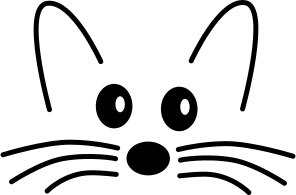
\includegraphics[width=1.4em]{squeak-logo}}}
\newcommand{\dothis}[1]{%
	\medskip
	\noindent\dothisicon
	\ifx#1\empty\else\quad\emph{#1}\fi
	\par\smallskip\nopagebreak}
% NB: To use this in an individual chapter, you must set:
%\graphicspath{{figures/} {../figures/}}
% at the head of the chapter.  Don't forget the final /
%=============================================================
%:Reader hints (hint)
%
% Indicates a non-obvious consequence 
\newcommand{\hint}[1]{\vspace{1ex}\noindent\fbox{\textsc{Astuce}} \emph{#1}}
%=================================================================
% graphics for Morphic handles
\newcommand{\grabHandle}{\raisebox{-0.2ex}{
\includegraphics[width=1em]{blackHandle}}}
\newcommand{\moveHandle}{\raisebox{-0.2ex}{
\includegraphics[width=1em]{moveHandle}}}
\newcommand{\debugHandle}{\raisebox{-0.2ex}{
\includegraphics[width=1em]{debugHandle}}}
% squeak-fr (added for Morphic handles)
\newcommand{\rotateHandle}{\raisebox{-0.2ex}{
\includegraphics[width=1em]{rotateHandle}}}
\newcommand{\viewerHandle}{\raisebox{-0.2ex}{
\includegraphics[width=1em]{viewerHandle}}}
% squeak-fr (add cloverHandle to use \clover in QuickTour.tex as alias
% todo 

%=============================================================
%:Highlighting Important stuff (doublebox)
%
% From Seaside book ...
\newsavebox{\SavedText}
\newlength{\InnerBoxRule}\setlength{\InnerBoxRule}{.75\fboxrule}
\newlength{\OuterBoxRule}\setlength{\OuterBoxRule}{1.5\fboxrule}
\newlength{\BoxSeparation}\setlength{\BoxSeparation}{1.5\fboxrule}
\addtolength{\BoxSeparation}{.5pt}
\newlength{\SaveBoxSep}\setlength{\SaveBoxSep}{2\fboxsep}
%
\newenvironment{doublebox}{\begin{lrbox}{\SavedText}
    \begin{minipage}{.75\textwidth}}
    {\end{minipage}\end{lrbox}\begin{center}
    \setlength{\fboxsep}{\BoxSeparation}\setlength{\fboxrule}{\OuterBoxRule}
    \fbox{\setlength{\fboxsep}{\SaveBoxSep}\setlength{\fboxrule}{\InnerBoxRule}%
      \fbox{\usebox{\SavedText}}}
  \end{center}}
% Use this:
%\newcommand{\important}[1]{\begin{doublebox}#1\end{doublebox}}


\newcommand{\important}[1]{
\noindent\rule{\textwidth}{2pt}\par
\textbf{Important!} #1 \par
\noindent\rule{\textwidth}{2pt}}

\newcommand{\note}[1]{
\noindent\rule{\textwidth}{2pt}\par
\noindent\textbf{Note} #1\par
\noindent\rule{\textwidth}{2pt}}

%=============================================================
%:Section depth
\setcounter{secnumdepth}{2}
%% for this to happen start the file with
%\ifx\wholebook\relax\else
%% $Author$ Martial
% $Date$ Wed Oct 10 13:34:55 CEST 2007
% $Revision$ source: SBE 12715 
% Last Changed Date: 2007-10-08 21:32:45 +0200 (Mon, 08 Oct 2007)
%=============================================================
% NB: documentclass must be set in main document.
% Allows book to be generated in multiple formats.
%=============================================================
%:Packages
%\usepackage[french]{babel}
\usepackage[T1]{fontenc}  %%%%%% really important to get the code directly in the text!
\usepackage{lmodern}
%\usepackage[scaled=0.85]{bookmanx} % needs another scale factor if used with \renewcommand{\sfdefault}{cmbr}
\usepackage{palatino}
%\usepackage[sc]{mathpazo}
%\linespread{1.05}
\usepackage[scaled=0.85]{helvet}
\usepackage{microtype}
\usepackage{graphicx}
\usepackage{theorem}
\usepackage[utf8]{inputenc}
% ON: pdfsync breaks the use of p{width} for tabular columns!
\ifdefined\usepdfsync\usepackage{pdfsync}\fi % Requires texlive 2007
%=============================================================
%:More packages
%Stef should check which ones are used!
%\usepackage{picinpar}
%\usepackage{layout}
%\usepackage{color}
%\definecolor{stefgris}{rgb}{0.85,0.85,0.85}
%\usepackage{enum}
%\usepackage{a4wide}
% \usepackage{fancyhdr}
\usepackage{ifthen}
\usepackage{float}
\usepackage{longtable}
\usepackage{makeidx}
\usepackage[nottoc]{tocbibind}
\usepackage{multicol}
\usepackage{booktabs}	% book-style tables
\usepackage{topcapt}	% enables \topcaption
\usepackage{multirow}
\usepackage{tabularx}
%\usepackage[bottom]{footmisc}
\usepackage{xspace}
\usepackage{alltt}
\usepackage{amssymb,textcomp}
\usepackage[usenames,dvipsnames]{color}
\usepackage{colortbl}
\usepackage[hang]{subfigure}\makeatletter\def\p@subfigure{\thefigure\,}\makeatother
\usepackage{rotating}
\usepackage{enumitem}	% apb: allows more control over tags in enumerations
\usepackage{verbatim}     % for comment environment
\usepackage{varioref}	% for page references that work
\labelformat{footnote}{\thechapter--#1} % to distinguish citations from jurabib
\usepackage{needspace}
\usepackage{isodateo} % enable \isodate
\usepackage[newparttoc]{titlesec}
\usepackage{titletoc}
\usepackage{eurosym}
\usepackage{wrapfig}

\usepackage[
	super,
	citefull=first,
	authorformat={allreversed,and},
	titleformat={commasep,italic}
]{jurabib} % citations as footnotes
\usepackage[
	colorlinks=true,
	linkcolor=black,
	urlcolor=black,
	citecolor=black
]{hyperref}   % should come last

%=============================================================
%:URL style
\makeatletter

\def\url@leostyle{%
  \@ifundefined{selectfont}{\def\UrlFont{\sf}}{\def\UrlFont{\sffamily}}}
% ajouter par Martial pour \traduit (met une dague dans les \doublebox
\def\thempfootnote{\fnsymbol{mpfootnote}}

\makeatother
% Now actually use the newly defined style.
\urlstyle{leo}
%=============================================================
%:Booleans
\newboolean{lulu}
\setboolean{lulu}{false}
\newcommand{\ifluluelse}[2]{\ifthenelse{\boolean{lulu}}{#1}{#2}}
%=============================================================
%:Names
\newcommand{\SUnit}{SUnit\xspace}
\newcommand{\sunit}{SUnit\xspace}
\newcommand{\xUnit}{$x$Unit\xspace}
\newcommand{\JUnit}{JUnit\xspace}
%\newcommand{\XP}{eXtreme Programming\xspace}
\newcommand{\st}{Smalltalk\xspace}
\newcommand{\Squeak}{Squeak\xspace}
\newcommand{\sq}{Squeak\xspace}
\newcommand{\sqmap}{SqueakMap\xspace}
\newcommand{\squeak}{Squeak\xspace}
%\newcommand{\sbe}{\url{scg.unibe.ch/SBE}\xspace}
%\newcommand{\sbe}{\url{squeakbyexample.org}\xspace}
\newcommand{\sbe}{\url{SqueakByExample.org}\xspace}
% squeak-fr: adresse de la version francaise
\newcommand{\spe}{\url{SqueakByExample.org/fr}\xspace}
\newcommand{\sba}{\url{SquareBracketAssociates.org}\xspace}

% squeak-fr: ajout de la \squeakdev pour eviter les problemes de
% changements d'url rencontres dans la VO:
\newcommand{\squeakdev}{\url{www.squeaksource.com/ImageForDevelopers}\xspace} %ou
%\newcommand{\squeakdev}{\url{squeak.ofset.org/squeak-dev}\xspace}

%=============================================================
%:Editorial comment macros
\newcommand{\nnbb}[2]{
    \fbox{\bfseries\sffamily\scriptsize#1}
    {\sf\small$\blacktriangleright$\textit{#2}$\blacktriangleleft$}
   }
\newcommand{\ab}[1]{\nnbb{Andrew}{#1}}
\newcommand{\sd}[1]{\nnbb{St\'{e}f}{#1}}
\newcommand{\md}[1]{\nnbb{Marcus}{#1}}
\newcommand{\on}[1]{\nnbb{Oscar}{#1}}
\newcommand{\damien}[1]{\nnbb{Damien}{#1}}
\newcommand{\lr}[1]{\nnbb{Lukas}{#1}}
\newcommand{\orla}[1]{\nnbb{Orla}{#1}}
%\newcommand{\here}{\nnbb{CONTINUE}{HERE}}
\newcommand{\here}{\nnbb{CONTINUE}{ICI}}

%=============================================================
%:Abbreviation macros
\newcommand{\ie}{\emph{c-\`a-d.}\xspace}
\newcommand{\cad}{\emph{c-\`a-d.}\xspace}
%\newcommand{\eg}{\emph{e.g.},\xspace}
\newcommand{\eg}{\emph{par ex.},\xspace}
\newcommand{\parex}{\emph{par ex.},\xspace}
\newcommand{\etc}{etc\xspace}
%=============================================================
%:Cross reference macros

% [squeak-fr] martial: remarquez les articles devant les noms
\newcommand{\charef}[1]{le chapitre~\ref{cha:#1}\xspace}
% note de martial: utilise dans chapitre Syntax.tex: a redefinir
\newcommand{\charefs}[2]{les chapitres~\ref{cha:#1} et \ref{cha:#2}\xspace}
\newcommand{\secref}[1]{la section~\ref{sec:#1}\xspace}
\newcommand{\figref}[1]{la figure~\ref{fig:#1}\xspace}
\newcommand{\Figref}[1]{La figure~\ref{fig:#1}\xspace}
\newcommand{\appref}[1]{l'annexe~\ref{app:#1}\xspace}
\newcommand{\tabref}[1]{la table~\ref{tab:#1}\xspace}
% defini pour le chapitre Messages.tex
\newcommand{\Tabref}[1]{La table~\ref{tab:#1}\xspace}

% APB: I removed trailing \xspace commands from these macros because
% \xspace mostly doesn't work.  If you want a space after your
% references, type one!
% ON: xspace has always worked just fine for me!  Please leave them in.
%
\newcommand{\ruleref}[1]{\ref{rule:#1}\xspace}
%
\newcommand{\egref}[1]{exemple~\ref{eg:#1}\xspace}
\newcommand{\Egref}[1]{Exemple~\ref{eg:#1}\xspace}
%
\newcommand{\scrref}[1]{script~\ref{scr:#1}\xspace}
\newcommand{\Scrref}[1]{Script~\ref{scr:#1}\xspace}
% t = the
\newcommand{\tscrref}[1]{le script~\ref{scr:#1}\xspace}
\newcommand{\Tscrref}[1]{Le script~\ref{scr:#1}\xspace}
%
\newcommand{\mthref}[1]{m\'ethode~\ref{mth:#1}\xspace}
\newcommand{\mthsref}[1]{m\'ethodes~\ref{mth:#1}\xspace}
\newcommand{\Mthref}[1]{M\'ethode~\ref{mth:#1}\xspace}
\newcommand{\tmthref}[1]{la m\'ethode~\ref{mth:#1}\xspace}
\newcommand{\Tmthref}[1]{La m\'ethode~\ref{mth:#1}\xspace}
%
\newcommand{\clsref}[1]{classe~\ref{cls:#1}\xspace}
\newcommand{\tclsref}[1]{la classe~\ref{cls:#1}\xspace}
\newcommand{\Tclsref}[1]{La classe~\ref{cls:#1}\xspace}
%=============================================================
%:Menu item macro
% for menu items, so we can change our minds on how to print them! (apb)
\definecolor{lightgray}{gray}{0.89}
\newcommand{\menu}[1]{{%
	\setlength{\fboxsep}{0pt}%
	\colorbox{lightgray}{{{\upshape\sffamily\strut \,#1\,}}}}}
% \newcommand{\menu}[1]{{%
% 	\fontfamily{lmr}\selectfont
% 	\upshape\textlangle{\sffamily #1}\textrangle}}
% For submenu items:
\newcommand{\go}{\,$\triangleright$\,}
% \newcommand{\go}{\,$\blacktriangleright$\,}
% For keyboard shortcuts:
%\newcommand{\short}[1]{\mbox{$\langle${\sc CMD}$\rangle$-#1}\xspace}
\newcommand{\short}[1]{\mbox{{\sc cmd}\hspace{0.08em}--\hspace{0.09em}#1}\xspace}
% For buttons:
\newcommand{\button}[1]{{%
	\setlength{\fboxsep}{0pt}%
	\fbox{{\upshape\sffamily\strut \,#1\,}}}}
\newcommand{\toolsflap}{l'onglet \textit{Tools}\xspace}
%=============================================================
%:Reader cues (do this)
%
% Indicate something the reader should try out.
\newcommand{\dothisicon}{\raisebox{-.5ex}{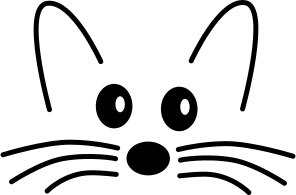
\includegraphics[width=1.4em]{squeak-logo}}}
\newcommand{\dothis}[1]{%
	\medskip
	\noindent\dothisicon
	\ifx#1\empty\else\quad\emph{#1}\fi
	\par\smallskip\nopagebreak}
% NB: To use this in an individual chapter, you must set:
%\graphicspath{{figures/} {../figures/}}
% at the head of the chapter.  Don't forget the final /
%=============================================================
%:Reader hints (hint)
%
% Indicates a non-obvious consequence 
\newcommand{\hint}[1]{\vspace{1ex}\noindent\fbox{\textsc{Astuce}} \emph{#1}}
%=================================================================
% graphics for Morphic handles
\newcommand{\grabHandle}{\raisebox{-0.2ex}{
\includegraphics[width=1em]{blackHandle}}}
\newcommand{\moveHandle}{\raisebox{-0.2ex}{
\includegraphics[width=1em]{moveHandle}}}
\newcommand{\debugHandle}{\raisebox{-0.2ex}{
\includegraphics[width=1em]{debugHandle}}}
% squeak-fr (added for Morphic handles)
\newcommand{\rotateHandle}{\raisebox{-0.2ex}{
\includegraphics[width=1em]{rotateHandle}}}
\newcommand{\viewerHandle}{\raisebox{-0.2ex}{
\includegraphics[width=1em]{viewerHandle}}}
% squeak-fr (add cloverHandle to use \clover in QuickTour.tex as alias
% todo 

%=============================================================
%:Highlighting Important stuff (doublebox)
%
% From Seaside book ...
\newsavebox{\SavedText}
\newlength{\InnerBoxRule}\setlength{\InnerBoxRule}{.75\fboxrule}
\newlength{\OuterBoxRule}\setlength{\OuterBoxRule}{1.5\fboxrule}
\newlength{\BoxSeparation}\setlength{\BoxSeparation}{1.5\fboxrule}
\addtolength{\BoxSeparation}{.5pt}
\newlength{\SaveBoxSep}\setlength{\SaveBoxSep}{2\fboxsep}
%
\newenvironment{doublebox}{\begin{lrbox}{\SavedText}
    \begin{minipage}{.75\textwidth}}
    {\end{minipage}\end{lrbox}\begin{center}
    \setlength{\fboxsep}{\BoxSeparation}\setlength{\fboxrule}{\OuterBoxRule}
    \fbox{\setlength{\fboxsep}{\SaveBoxSep}\setlength{\fboxrule}{\InnerBoxRule}%
      \fbox{\usebox{\SavedText}}}
  \end{center}}
% Use this:
%\newcommand{\important}[1]{\begin{doublebox}#1\end{doublebox}}


\newcommand{\important}[1]{
\noindent\rule{\textwidth}{2pt}\par
\textbf{Important!} #1 \par
\noindent\rule{\textwidth}{2pt}}

\newcommand{\note}[1]{
\noindent\rule{\textwidth}{2pt}\par
\noindent\textbf{Note} #1\par
\noindent\rule{\textwidth}{2pt}}

%=============================================================
%:Section depth
\setcounter{secnumdepth}{2}
%% for this to happen start the file with
%\ifx\wholebook\relax\else
%% $Author$ Martial
% $Date$ Wed Oct 10 13:34:55 CEST 2007
% $Revision$ source: SBE 12715 
% Last Changed Date: 2007-10-08 21:32:45 +0200 (Mon, 08 Oct 2007)
%=============================================================
% NB: documentclass must be set in main document.
% Allows book to be generated in multiple formats.
%=============================================================
%:Packages
%\usepackage[french]{babel}
\usepackage[T1]{fontenc}  %%%%%% really important to get the code directly in the text!
\usepackage{lmodern}
%\usepackage[scaled=0.85]{bookmanx} % needs another scale factor if used with \renewcommand{\sfdefault}{cmbr}
\usepackage{palatino}
%\usepackage[sc]{mathpazo}
%\linespread{1.05}
\usepackage[scaled=0.85]{helvet}
\usepackage{microtype}
\usepackage{graphicx}
\usepackage{theorem}
\usepackage[utf8]{inputenc}
% ON: pdfsync breaks the use of p{width} for tabular columns!
\ifdefined\usepdfsync\usepackage{pdfsync}\fi % Requires texlive 2007
%=============================================================
%:More packages
%Stef should check which ones are used!
%\usepackage{picinpar}
%\usepackage{layout}
%\usepackage{color}
%\definecolor{stefgris}{rgb}{0.85,0.85,0.85}
%\usepackage{enum}
%\usepackage{a4wide}
% \usepackage{fancyhdr}
\usepackage{ifthen}
\usepackage{float}
\usepackage{longtable}
\usepackage{makeidx}
\usepackage[nottoc]{tocbibind}
\usepackage{multicol}
\usepackage{booktabs}	% book-style tables
\usepackage{topcapt}	% enables \topcaption
\usepackage{multirow}
\usepackage{tabularx}
%\usepackage[bottom]{footmisc}
\usepackage{xspace}
\usepackage{alltt}
\usepackage{amssymb,textcomp}
\usepackage[usenames,dvipsnames]{color}
\usepackage{colortbl}
\usepackage[hang]{subfigure}\makeatletter\def\p@subfigure{\thefigure\,}\makeatother
\usepackage{rotating}
\usepackage{enumitem}	% apb: allows more control over tags in enumerations
\usepackage{verbatim}     % for comment environment
\usepackage{varioref}	% for page references that work
\labelformat{footnote}{\thechapter--#1} % to distinguish citations from jurabib
\usepackage{needspace}
\usepackage{isodateo} % enable \isodate
\usepackage[newparttoc]{titlesec}
\usepackage{titletoc}
\usepackage{eurosym}
\usepackage{wrapfig}

\usepackage[
	super,
	citefull=first,
	authorformat={allreversed,and},
	titleformat={commasep,italic}
]{jurabib} % citations as footnotes
\usepackage[
	colorlinks=true,
	linkcolor=black,
	urlcolor=black,
	citecolor=black
]{hyperref}   % should come last

%=============================================================
%:URL style
\makeatletter

\def\url@leostyle{%
  \@ifundefined{selectfont}{\def\UrlFont{\sf}}{\def\UrlFont{\sffamily}}}
% ajouter par Martial pour \traduit (met une dague dans les \doublebox
\def\thempfootnote{\fnsymbol{mpfootnote}}

\makeatother
% Now actually use the newly defined style.
\urlstyle{leo}
%=============================================================
%:Booleans
\newboolean{lulu}
\setboolean{lulu}{false}
\newcommand{\ifluluelse}[2]{\ifthenelse{\boolean{lulu}}{#1}{#2}}
%=============================================================
%:Names
\newcommand{\SUnit}{SUnit\xspace}
\newcommand{\sunit}{SUnit\xspace}
\newcommand{\xUnit}{$x$Unit\xspace}
\newcommand{\JUnit}{JUnit\xspace}
%\newcommand{\XP}{eXtreme Programming\xspace}
\newcommand{\st}{Smalltalk\xspace}
\newcommand{\Squeak}{Squeak\xspace}
\newcommand{\sq}{Squeak\xspace}
\newcommand{\sqmap}{SqueakMap\xspace}
\newcommand{\squeak}{Squeak\xspace}
%\newcommand{\sbe}{\url{scg.unibe.ch/SBE}\xspace}
%\newcommand{\sbe}{\url{squeakbyexample.org}\xspace}
\newcommand{\sbe}{\url{SqueakByExample.org}\xspace}
% squeak-fr: adresse de la version francaise
\newcommand{\spe}{\url{SqueakByExample.org/fr}\xspace}
\newcommand{\sba}{\url{SquareBracketAssociates.org}\xspace}

% squeak-fr: ajout de la \squeakdev pour eviter les problemes de
% changements d'url rencontres dans la VO:
\newcommand{\squeakdev}{\url{www.squeaksource.com/ImageForDevelopers}\xspace} %ou
%\newcommand{\squeakdev}{\url{squeak.ofset.org/squeak-dev}\xspace}

%=============================================================
%:Editorial comment macros
\newcommand{\nnbb}[2]{
    \fbox{\bfseries\sffamily\scriptsize#1}
    {\sf\small$\blacktriangleright$\textit{#2}$\blacktriangleleft$}
   }
\newcommand{\ab}[1]{\nnbb{Andrew}{#1}}
\newcommand{\sd}[1]{\nnbb{St\'{e}f}{#1}}
\newcommand{\md}[1]{\nnbb{Marcus}{#1}}
\newcommand{\on}[1]{\nnbb{Oscar}{#1}}
\newcommand{\damien}[1]{\nnbb{Damien}{#1}}
\newcommand{\lr}[1]{\nnbb{Lukas}{#1}}
\newcommand{\orla}[1]{\nnbb{Orla}{#1}}
%\newcommand{\here}{\nnbb{CONTINUE}{HERE}}
\newcommand{\here}{\nnbb{CONTINUE}{ICI}}

%=============================================================
%:Abbreviation macros
\newcommand{\ie}{\emph{c-\`a-d.}\xspace}
\newcommand{\cad}{\emph{c-\`a-d.}\xspace}
%\newcommand{\eg}{\emph{e.g.},\xspace}
\newcommand{\eg}{\emph{par ex.},\xspace}
\newcommand{\parex}{\emph{par ex.},\xspace}
\newcommand{\etc}{etc\xspace}
%=============================================================
%:Cross reference macros

% [squeak-fr] martial: remarquez les articles devant les noms
\newcommand{\charef}[1]{le chapitre~\ref{cha:#1}\xspace}
% note de martial: utilise dans chapitre Syntax.tex: a redefinir
\newcommand{\charefs}[2]{les chapitres~\ref{cha:#1} et \ref{cha:#2}\xspace}
\newcommand{\secref}[1]{la section~\ref{sec:#1}\xspace}
\newcommand{\figref}[1]{la figure~\ref{fig:#1}\xspace}
\newcommand{\Figref}[1]{La figure~\ref{fig:#1}\xspace}
\newcommand{\appref}[1]{l'annexe~\ref{app:#1}\xspace}
\newcommand{\tabref}[1]{la table~\ref{tab:#1}\xspace}
% defini pour le chapitre Messages.tex
\newcommand{\Tabref}[1]{La table~\ref{tab:#1}\xspace}

% APB: I removed trailing \xspace commands from these macros because
% \xspace mostly doesn't work.  If you want a space after your
% references, type one!
% ON: xspace has always worked just fine for me!  Please leave them in.
%
\newcommand{\ruleref}[1]{\ref{rule:#1}\xspace}
%
\newcommand{\egref}[1]{exemple~\ref{eg:#1}\xspace}
\newcommand{\Egref}[1]{Exemple~\ref{eg:#1}\xspace}
%
\newcommand{\scrref}[1]{script~\ref{scr:#1}\xspace}
\newcommand{\Scrref}[1]{Script~\ref{scr:#1}\xspace}
% t = the
\newcommand{\tscrref}[1]{le script~\ref{scr:#1}\xspace}
\newcommand{\Tscrref}[1]{Le script~\ref{scr:#1}\xspace}
%
\newcommand{\mthref}[1]{m\'ethode~\ref{mth:#1}\xspace}
\newcommand{\mthsref}[1]{m\'ethodes~\ref{mth:#1}\xspace}
\newcommand{\Mthref}[1]{M\'ethode~\ref{mth:#1}\xspace}
\newcommand{\tmthref}[1]{la m\'ethode~\ref{mth:#1}\xspace}
\newcommand{\Tmthref}[1]{La m\'ethode~\ref{mth:#1}\xspace}
%
\newcommand{\clsref}[1]{classe~\ref{cls:#1}\xspace}
\newcommand{\tclsref}[1]{la classe~\ref{cls:#1}\xspace}
\newcommand{\Tclsref}[1]{La classe~\ref{cls:#1}\xspace}
%=============================================================
%:Menu item macro
% for menu items, so we can change our minds on how to print them! (apb)
\definecolor{lightgray}{gray}{0.89}
\newcommand{\menu}[1]{{%
	\setlength{\fboxsep}{0pt}%
	\colorbox{lightgray}{{{\upshape\sffamily\strut \,#1\,}}}}}
% \newcommand{\menu}[1]{{%
% 	\fontfamily{lmr}\selectfont
% 	\upshape\textlangle{\sffamily #1}\textrangle}}
% For submenu items:
\newcommand{\go}{\,$\triangleright$\,}
% \newcommand{\go}{\,$\blacktriangleright$\,}
% For keyboard shortcuts:
%\newcommand{\short}[1]{\mbox{$\langle${\sc CMD}$\rangle$-#1}\xspace}
\newcommand{\short}[1]{\mbox{{\sc cmd}\hspace{0.08em}--\hspace{0.09em}#1}\xspace}
% For buttons:
\newcommand{\button}[1]{{%
	\setlength{\fboxsep}{0pt}%
	\fbox{{\upshape\sffamily\strut \,#1\,}}}}
\newcommand{\toolsflap}{l'onglet \textit{Tools}\xspace}
%=============================================================
%:Reader cues (do this)
%
% Indicate something the reader should try out.
\newcommand{\dothisicon}{\raisebox{-.5ex}{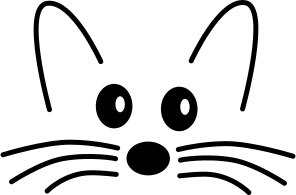
\includegraphics[width=1.4em]{squeak-logo}}}
\newcommand{\dothis}[1]{%
	\medskip
	\noindent\dothisicon
	\ifx#1\empty\else\quad\emph{#1}\fi
	\par\smallskip\nopagebreak}
% NB: To use this in an individual chapter, you must set:
%\graphicspath{{figures/} {../figures/}}
% at the head of the chapter.  Don't forget the final /
%=============================================================
%:Reader hints (hint)
%
% Indicates a non-obvious consequence 
\newcommand{\hint}[1]{\vspace{1ex}\noindent\fbox{\textsc{Astuce}} \emph{#1}}
%=================================================================
% graphics for Morphic handles
\newcommand{\grabHandle}{\raisebox{-0.2ex}{
\includegraphics[width=1em]{blackHandle}}}
\newcommand{\moveHandle}{\raisebox{-0.2ex}{
\includegraphics[width=1em]{moveHandle}}}
\newcommand{\debugHandle}{\raisebox{-0.2ex}{
\includegraphics[width=1em]{debugHandle}}}
% squeak-fr (added for Morphic handles)
\newcommand{\rotateHandle}{\raisebox{-0.2ex}{
\includegraphics[width=1em]{rotateHandle}}}
\newcommand{\viewerHandle}{\raisebox{-0.2ex}{
\includegraphics[width=1em]{viewerHandle}}}
% squeak-fr (add cloverHandle to use \clover in QuickTour.tex as alias
% todo 

%=============================================================
%:Highlighting Important stuff (doublebox)
%
% From Seaside book ...
\newsavebox{\SavedText}
\newlength{\InnerBoxRule}\setlength{\InnerBoxRule}{.75\fboxrule}
\newlength{\OuterBoxRule}\setlength{\OuterBoxRule}{1.5\fboxrule}
\newlength{\BoxSeparation}\setlength{\BoxSeparation}{1.5\fboxrule}
\addtolength{\BoxSeparation}{.5pt}
\newlength{\SaveBoxSep}\setlength{\SaveBoxSep}{2\fboxsep}
%
\newenvironment{doublebox}{\begin{lrbox}{\SavedText}
    \begin{minipage}{.75\textwidth}}
    {\end{minipage}\end{lrbox}\begin{center}
    \setlength{\fboxsep}{\BoxSeparation}\setlength{\fboxrule}{\OuterBoxRule}
    \fbox{\setlength{\fboxsep}{\SaveBoxSep}\setlength{\fboxrule}{\InnerBoxRule}%
      \fbox{\usebox{\SavedText}}}
  \end{center}}
% Use this:
%\newcommand{\important}[1]{\begin{doublebox}#1\end{doublebox}}


\newcommand{\important}[1]{
\noindent\rule{\textwidth}{2pt}\par
\textbf{Important!} #1 \par
\noindent\rule{\textwidth}{2pt}}

\newcommand{\note}[1]{
\noindent\rule{\textwidth}{2pt}\par
\noindent\textbf{Note} #1\par
\noindent\rule{\textwidth}{2pt}}

%=============================================================
%:Section depth
\setcounter{secnumdepth}{2}
%% for this to happen start the file with
%\ifx\wholebook\relax\else
%\input{../common.tex}
%\begin{document}
%\fi
% and terminate by
% \ifx\wholebook\relax\else\end{document}\fi

\DeclareGraphicsExtensions{.pdf, .jpg, .png}
%=============================================================
%:PDF setup
\hypersetup{
%   a4paper,
%   pdfstartview=FitV,
%   colorlinks,
%   linkcolor=darkblue,
%   citecolor=darkblue,
%   pdftitle={Squeak by Example},
pdftitle={Squeak par l'exemple},
   pdfauthor={Andrew Black, St\'ephane Ducasse,	Oscar Nierstrasz,
Damien Pollet},
   pdfkeywords={Smalltalk, Squeak, Programmation Orient\'ee Objet},
pdfsubject={Informatique, Computer Science}
}
%=============================================================
%:Page layout and appearance
%
% \renewcommand{\headrulewidth}{0pt}
\renewcommand{\chaptermark}[1]{\markboth{#1}{}}
\renewcommand{\sectionmark}[1]{\markright{\thesection\ #1}}
\renewpagestyle{plain}[\small\itshape]{%
	\setheadrule{0pt}%
	\sethead[][][]{}{}{}%
	\setfoot[][][]{}{}{}}
\renewpagestyle{headings}[\small\itshape]{%
	\setheadrule{0pt}%
	\setmarks{chapter}{section}%
	\sethead[\thepage][][\chaptertitle]{\sectiontitle}{}{\thepage}%
	\setfoot[][][]{}{}{}}
% pagestyle for tableofcontents + index (martial: 2008/04/23)
\newpagestyle{newheadings}[\small\itshape]{%
	\setheadrule{0pt}%
	\setmarks{chapter}{section}%
	\sethead[\thepage][][\chaptertitle]{\chaptertitle}{}{\thepage}%
	\setfoot[][][]{}{}{}}
%=============================================================
%:Title section setup and TOC numbering depth
\setcounter{secnumdepth}{1}
\setcounter{tocdepth}{1}
\titleformat{\part}[display]{\centering}{\huge\partname\ \thepart}{1em}{\Huge\textbf}[]
\titleformat{\chapter}[display]{}{\huge\chaptertitlename\ \thechapter}{1em}{\Huge\raggedright\textbf}[]
\titlecontents{part}[3pc]{%
		\pagebreak[2]\addvspace{1em plus.4em minus.2em}%
		\leavevmode\large\bfseries}
	{\contentslabel{3pc}}{\hspace*{-3pc}}
	{}[\nopagebreak]
\titlecontents{chapter}[3pc]{%
		\pagebreak[0]\addvspace{1em plus.2em minus.2em}%
		\leavevmode\bfseries}
	{\contentslabel{3pc}}{}
	{\hfill\contentspage}[\nopagebreak]
\dottedcontents{section}[3pc]{}{3pc}{1pc}
\dottedcontents{subsection}[3pc]{}{0pc}{1pc}
% \dottedcontents{subsection}[4.5em]{}{0pt}{1pc}
% Make \cleardoublepage insert really blank pages http://www.tex.ac.uk/cgi-bin/texfaq2html?label=reallyblank
\let\origdoublepage\cleardoublepage
\newcommand{\clearemptydoublepage}{%
  \clearpage
  {\pagestyle{empty}\origdoublepage}}
\let\cleardoublepage\clearemptydoublepage % see http://www.tex.ac.uk/cgi-bin/texfaq2html?label=patch
%=============================================================
%:FAQ macros (for FAQ chapter)
\newtheorem{faq}{FAQ}
\newcommand{\answer}{\paragraph{R\'eponse}\ }
%=============================================================
%:Listings package configuration
\usepackage{listings}
\newcommand{\caret}{\makebox{\raisebox{0.4ex}{\footnotesize{$\wedge$}}}}
\lstdefinelanguage{Smalltalk}{
%  morekeywords={self,super,true,false,nil,thisContext}, % This is overkill
  morestring=[d]',
  morecomment=[s]{"}{"},
  alsoletter={\#:},
  escapechar={!},
  escapebegin=\itshape, % comment-like by default (Martial 11/2007)
  literate=
    {BANG}{!}1
    {UNDERSCORE}{\_}1
    {\\st}{Smalltalk}9 % convenience -- in case \st occurs in code
    % {'}{{\textquotesingle}}1 % replaced by upquote=true in \lstset
    {_}{{$\leftarrow$}}1
    {>>>}{{\sep}}1
    {^}{{$\uparrow$}}1
    {~}{{$\sim$}}1
    {-}{{\sf -\hspace{-0.13em}-}}1  % the goal is to make - the same width as +
    {+}{\raisebox{0.08ex}{+}}1		% and to raise + off the baseline to match -
    {-->}{{\quad$\longrightarrow$\quad}}3
	, % Don't forget the comma at the end!
  tabsize=4
}[keywords,comments,strings]
% ajout pour les échappements dans les codes
% indispensable pour mettre le code en emphase (cf. Model.tex) 
\newcommand{\codeify}[1]{\NoAutoSpaceBeforeFDP#1\AutoSpaceBeforeFDP}
\newcommand{\normcomment}[1]{\emph{#1}} %cf. Streams
\newcommand{\normcode}[1]{\emph{\codeify{#1}}} %cf. Streams
\newcommand{\emcode}[1]{\textbf{\normcode{#1}}} % Martial 11/2007
\lstset{language=Smalltalk,
	basicstyle=\sffamily,
	keywordstyle=\color{black}\bfseries,
	% stringstyle=\ttfamily, % Ugly! do we really want this? -- on
	%commentstyle=\itshape,
	mathescape=true,
	showstringspaces=false,
	keepspaces=true,
	breaklines=true,
	breakautoindent=true,
	lineskip={-1pt}, % Ugly hack
	upquote=true, % straight quote; requires textcomp package
	columns=fullflexible} % no fixed width fonts
% In-line code (literal)
% Normally use this for all in-line code:
\newcommand{\ct}{\lstinline[mathescape=false,basicstyle={\sffamily\upshape}]}
% apb 2007.8.28 added the \upshape declaration to avoid getting italicized code in \dothis{ } sections.
% In-line code (latex enabled)
% Use this only in special situations where \ct does not work
% (within section headings ...):

% [squeak-fr] Modification de \lct suivant les indications de Martial Boniou
\newcommand{\lct}[1]{\textsf{\textup{\NoAutoSpaceBeforeFDP #1
\AutoSpaceBeforeFDP}}} %\xspace

% Use these for system categories and protocols:
\newcommand{\scat}[1]{\emph{\textsf{#1}}\xspace}
\newcommand{\pkg}[1]{\emph{\textsf{#1}}\xspace}
\newcommand{\prot}[1]{\emph{\textsf{#1}}\xspace}
% Code environments
% NB: the arg is for tests
% Only code and example environments may be tests
\lstnewenvironment{code}[1]{%
	\lstset{%
		frame=lines,
		mathescape=false
	}
}{}
\def\ignoredollar#1{}
%=============================================================
%:Code environments (method, script ...)
% NB: the third arg is for tests
% Only code and example environments may be tests
\lstnewenvironment{example}[3][defaultlabel]{%
	\renewcommand{\lstlistingname}{Exemple}%
	\lstset{
		frame=lines,
		mathescape=false,
		caption={\emph{#2}},
		label={eg:#1}
	}
}{}
\lstnewenvironment{script}[2][defaultlabel]{%
\renewcommand{\lstlistingname}{Script}%
	\lstset{
		frame=lines,
		mathescape=false,
		name={Script},
		caption={\emph{#2}},
		label={scr:#1}
	}
}{}
%I could not find a way yo get the Experiment #numb followed by the caption in a black box
%\colorbox{black}{\makebox[\textwidth]{  \color{white} {\large {\bfseries Experiment 3-1 (crear i moure un robot)}} }}
\lstnewenvironment{experiment}[2][defaultlabel]{%
%\noindent\rule{\textwidth}{2pt}\vspace{-0.8cm}
\renewcommand{\lstlistingname}{Experiment}%
	\lstset{
		frame=none,
		rulecolor=\color{black},
		mathescape=false,
		name={Experiment},
		caption={\emph{#2}},
		label={scr:#1}
	}
}{%\vspace{-0.5cm}\noindent\rule{\textwidth}{2pt}
}

\lstnewenvironment{method}[2][defaultlabel]{%
	\renewcommand{\lstlistingname}{Method}%
	\lstset{
		frame=lines,
		mathescape=false,
		name={M\'ethode},
		caption={\emph{#2}},
		label={mth:#1}
	}
}{}
\lstnewenvironment{methods}[2][defaultlabel]{% just for multiple methods at once
	\renewcommand{\lstlistingname}{Methods}%
	\lstset{
		frame=lines,
		mathescape=false,
		name={M\'ethode},
		caption={\emph{#2}},
		label={mth:#1}
	}
}{}
\lstnewenvironment{numMethod}[2][defaultlabel]{%
	\renewcommand{\lstlistingname}{Method}%
	\lstset{
		numbers=left,
		numberstyle={\tiny\sffamily},
		frame=lines,
		mathescape=false,
		name={M\'ethode},
		caption={\emph{#2}},
		label={mth:#1}
	}
}{}
% \lstnewenvironment{classdef}[2][defaultlabel]{%
% 	\renewcommand{\lstlistingname}{Classe}%
% 	\lstset{
% 		frame=lines,
% 		mathescape=false,
% 		name={Classe},
% 		caption={\emph{#2}},
% 		label={cls:#1}
% 	}
% }{}

%%%%%%%%%%%%%%%%%%%%%%%%%%%%%%%%%%%%%%%%%%%%%%%%%%%%%%%%%%%%%%%%%%%%%%%%%%%%%%%%%%%%%%%%%%%%%%%%%
%%From the original book latex template
%%%%%%%%%%%%%%%%%%%%%%%%%%%%%%%%%%%%%%%%%%%%%%%%%%%%%%%%%%%%%%%%%%%%%%%%%%%%%%%%%%%%%%%%%%%%%%%%%
\theoremstyle{break}
{\theorembodyfont{\rmfamily}\theoremstyle{break}
\newtheorem{privScript}{Script}[chapter]
%\newtheorem{privMethod}{Method}[chapter]
\newtheorem{privExercise}{Experiment}[chapter]}

% \theoremstyle{break}
% {\theorembodyfont{\rmfamily} \newtheorem{privMethod}{Method}[chapter]}

%class
\theoremstyle{break}
{\theorembodyfont{\rmfamily} \newtheorem{privClassDef}{Class}[chapter]}

%important
\theoremstyle{break}
{\theorembodyfont{\rmfamily} \newtheorem{privTemplate}{Important Messages}[chapter]}

% experiment
\newenvironment{exercise}
    {\begin{privExercise}\mbox{}\\}
    {\end{privExercise}}


%%% for figure
\newsavebox{\ScriptFigure}
\newlength{\ScriptWidth}
\newlength{\FigureWidth}

%%%%%%%%%%%%%%%%%%%%%%%%%%%%%%%%%%%%%%%%%%%%%%%%%%%%%%%%%%%%%%%%%%%%%%%%%%%%%%%%
\newenvironment{scriptfig}[3][0.6]
   {\setlength{\ScriptWidth}{\linewidth*\real{#1}}%
   \setlength{\FigureWidth}{\linewidth-(\linewidth*\real{#1})}%
   \savebox{\ScriptFigure}%
	{\parbox{\FigureWidth}{\includegraphics[width=0.98\FigureWidth]{#2}}}%
   \par\noindent\begin{minipage}{\linewidth}\hrule\vskip 0.2cm\begin{minipage}[c]{\ScriptWidth}%
   \begin{stefscript}[{\em #3}]\begin{alltt}\sffamily}
   {\end{alltt}\end{stefscript}\end{minipage}\hfill
   \usebox{\ScriptFigure}
   \vskip 1ex\hrule\end{minipage}\vskip 1ex\par}

%%%%%%%%%%%%%%%%%%%%%%%%%%%%%%%%%%%%%%%%%%%%%%%%%%%%%%%%%%%%%%%%%%%%%%%%%%%%%%%%
%% to be able to specify the complete set of values for includegraphics
%% may be will be changed but not the interface
\newenvironment{scriptfigwithsize}[3][0.6]
   {\setlength{\ScriptWidth}{\linewidth*\real{#1}}%
   \setlength{\FigureWidth}{\linewidth-(\linewidth*\real{#1})}%
   \savebox{\ScriptFigure}{\parbox{\FigureWidth}{\raggedleft{#2}}}%
   \par\noindent\begin{minipage}{\linewidth}\hrule\vskip 0.3cm\begin{minipage}[c]{\ScriptWidth}%
   \begin{stefscript}[{\em #3}]\begin{alltt}\sffamily}
   {\end{alltt}\end{stefscript}\end{minipage}\hfill
   \usebox{\ScriptFigure}
   \vskip 1ex\hrule\end{minipage}\vskip 1ex\par}

% \newenvironment{methodfig}[2][0.6]
%    {\setlength{\ScriptWidth}{\linewidth*\real{#1}}%
%    \setlength{\FigureWidth}{\linewidth-(\linewidth*\real{#1})}%
%    \savebox{\ScriptFigure}{\parbox{\FigureWidth}{\includegraphics[width=.98\FigureWidth]{#2}}}%
%    \par\noindent\rule{\linewidth}{1mm}
%    \\[-0.3cm]\noindent\rule{\linewidth}{0.1mm}
%    \noindent\begin{minipage}[c]{\ScriptWidth}\begin{privMethod}\begin{alltt}\sffamily}
%    {\end{alltt}\end{privMethod}\end{minipage}\hfill
%    \usebox{\ScriptFigure} \vskip 1ex\hrule\vskip 1ex\par}

% \newenvironment{method}
% {\par\noindent\begin{minipage}{\linewidth}\vspace{0.2cm}\begin{privMethod}\begin{nminipage}\vspace{-0.2cm}\rule{\linewidth}{1mm}\\[-0.6cm]\rule{\linewidth}{0.1mm}\end{nminipage}\hspace*{\scriptindent}\codesize\begin{nalltt}\vspace{-0.2cm}}
% {\end{nalltt}\normalsize\vspace{-0.1cm}\hrule\end{privMethod}\vspace{0.2cm}\end{minipage}}


% \newenvironment{classdef}
% {\par\noindent\begin{minipage}{\linewidth}\vspace{0.2cm}\begin{privClassDef}\begin{nminipage}\vspace{-0.2cm}\rule{\linewidth}{1mm}\\[-0.6cm]\rule{\linewidth}{0.1mm}\end{nminipage}\hspace*{\scriptindent}\codesize\begin{nalltt}\vspace{-0.2cm}}
% {\end{nalltt}\normalsize\vspace{-0.1cm}\hrule\end{privClassDef}\vspace{0.2cm}\end{minipage}}


% \newenvironment{template}
% {\par\noindent\begin{minipage}{\linewidth}\vspace{0.3cm}\begin{privTemplate}\begin{nminipage}\vspace{-0.4cm}\rule{\linewidth}{0.1mm}\end{nminipage}\hspace*{\scriptindent}\begin{nalltt}\vspace{-0.7cm}}
% {\end{nalltt}\vspace{-0.1cm}\hrule\end{privTemplate}\end{minipage}\vspace{0.3cm}}

\newenvironment{exofig}[2][0.7]
   {\setlength{\ScriptWidth}{\linewidth*\real{#1}}
   \setlength{\FigureWidth}{\linewidth-(\linewidth*\real{#1})}
   \savebox{\ScriptFigure}{\parbox{\FigureWidth}{\raggedleft{\includegraphics[width=.98\FigureWidth]{#2}}}}
   \par\noindent\begin{minipage}{\linewidth}\hrule\vskip 0.3cm\begin{minipage}[c]{\ScriptWidth}%
   \begin{privExercise}}
   {\end{privExercise}\end{minipage}\hfill
   \usebox{\ScriptFigure}
   \vskip 1ex\hrule\end{minipage}\vskip 1ex\par}

\newenvironment{exofigwithsize}[2][0.7]
   {\setlength{\ScriptWidth}{\linewidth*\real{#1}}
   \setlength{\FigureWidth}{\linewidth-(\linewidth*\real{#1})}
   \savebox{\ScriptFigure}{\parbox{\FigureWidth}{\raggedleft{#2}}}
   \par\noindent\begin{minipage}{\linewidth}\hrule\vskip 0.3cm\begin{minipage}[c]{\ScriptWidth}%
   \begin{privExercise}}
   {\end{privExercise}\end{minipage}\hfill\usebox{\ScriptFigure}
   \vskip 1ex\hrule\end{minipage}\vskip 1ex\par}

\newenvironment{exofigwithsizeandtitle}[3][0.7]
   {\setlength{\ScriptWidth}{\linewidth*\real{#1}}
   \setlength{\FigureWidth}{\linewidth-(\linewidth*\real{#1})}
   \savebox{\ScriptFigure}{\parbox{\FigureWidth}{\raggedleft{#2}}}
   \vskip 0.3cm\par\noindent\begin{minipage}{\linewidth}\hrule\vskip 0.1cm\begin{minipage}[c]{\ScriptWidth}%
   \begin{privExercise}[\em{#3}]}
   {\end{privExercise}\end{minipage}\hfill\usebox{\ScriptFigure}
   \vskip 1ex\hrule\end{minipage}\vskip 1ex\par}

\newenvironment{exofigwithtitle}[3][0.7]
   {\setlength{\ScriptWidth}{\linewidth*\real{#1}}
   \setlength{\FigureWidth}{\linewidth-(\linewidth*\real{#1})}
   \savebox{\ScriptFigure}{\parbox{\FigureWidth}{\raggedleft{\includegraphics[width=.98\FigureWidth]{#2}}}}
   \par\noindent\begin{minipage}{\linewidth}\hrule\vskip 0.3cm\begin{minipage}[c]{\ScriptWidth}%
   \begin{privExercise}[\em{#3}]}
   {\end{privExercise}\end{minipage}\hfill
   \usebox{\ScriptFigure}
   \vskip 1ex\hrule\end{minipage}\vskip 1ex\par}


\newenvironment{exonofigwithtitle}[3][0.7]
   {\setlength{\ScriptWidth}{\linewidth*\real{#1}}
   \setlength{\FigureWidth}{\linewidth-(\linewidth*\real{#1})}
   \savebox{\ScriptFigure}{\parbox{\FigureWidth}{\raggedleft{\includegraphics[width=.98\FigureWidth]{#2}}}}
   \par\noindent\begin{minipage}{\linewidth}\hrule\vskip 0.3cm\begin{minipage}[c]{\ScriptWidth}%
   \begin{privExercise}[\em{#3}]}
   {\end{privExercise}\end{minipage}\hfill
   \usebox{\ScriptFigure}
   \vskip 1ex\hrule\end{minipage}\vskip 1ex\par}

\newenvironment{exonofig}
   {\par\noindent\begin{minipage}[t]{\linewidth}\noindent\begin{privExercise}}
   {\end{privExercise}\end{minipage}\vspace{0.5cm}\par}

\newenvironment{exonofigtitle}[1]
   {\par\noindent\begin{minipage}[t]{\linewidth}\noindent\begin{privExercise}[\em{#1}]}
   {\end{privExercise}\end{minipage}\vspace{0.5cm}\par}
		
% \newenvironment{solfig}[3][0.5]
%    {\setlength{\ScriptWidth}{\linewidth*\real{#1}}
%    \setlength{\FigureWidth}{\linewidth-\linewidth*\real{#1}}
%    \savebox{\ScriptFigure}{\parbox{\FigureWidth}{\includegraphics[width=.9\linewidth]{#2}}}
%    \par\noindent\vskip 1ex\hrule\vskip 1ex\begin{minipage}[t]{\ScriptWidth}
%    {\bf Solution #3} \begin{alltt}\sffamily}
%    {\end{alltt}\end{minipage}\hfill
%    \usebox{\ScriptFigure}
%    \vskip 1ex\hrule\vskip 1ex\par}
% 
% \newenvironment{solnofig}[1]
%    {\par\noindent\vskip 1ex\hrule\vskip 1ex\begin{minipage}[t]{\ScriptWidth}
%    {\bf Solution #1} \begin{alltt}\sffamily}
%    {\end{alltt}\end{minipage}\hfill
%    \vskip 1ex\hrule\vskip 1ex\par}
% 
% \newenvironment{exoscript}[3][0.5]
%    {\setlength{\ScriptWidth}{\linewidth*\real{#1}}
%     \setlength{\FigureWidth}{\linewidth-\linewidth*\real{#1}}
%     \savebox{\ScriptFigure}{\begin{minipage}\begin{alltt}\sffamily#3\end{alltt}\end{minipage}}
%     \par\noindent\vskip 1ex\hrule\vskip 1ex\begin{minipage}[t]{\ScriptWidth}
%     \begin{privExercise}}
%     {\end{privExercise}\end{minipage}\hfill
%     \usebox{\ScriptFigure}
% \vskip 1ex\hrule\vskip 1ex\par}


%%%%%%%%%%%%%%%%%%%%%%%%%%%%%%%%%%%%%%%%%%%%%%%%%%%%%%%%%%%%%%%%
%% Define the indentation from which the code script starts
%\newlength{\scriptindent}
%\setlength{\scriptindent}{.3cm}
%%%%%%%%%%%%%%%%%%%%%%%%%%%%%%%%%%%%%%%%%%%%%%%%%%%%%%%%%%%%%%%%
%% Method presentation 
%\newlength{\methodindent}
%\newlength{\methodwordlength}
%\newlength{\aftermethod}
%\setlength{\methodindent}{0.2cm}
%\settowidth{\methodwordlength}{\ M\'ethode\ }

%%%%%%%%%%%%%%%%%%%%%%%%%%%%%%%%%%%%%%%%%%%%%%%%%%%%%%%%%%%%%%%%
\theoremstyle{break}
{\theorembodyfont{\rmfamily} \newtheorem{fonction}{Script}[chapter]}

\newsavebox{\fminibox}
\newlength{\fminilength}
% Fait un truc encadre
\newenvironment{fminipage}[1][\linewidth]
  {\setlength{\fminilength}{#1-2\fboxsep-2\fboxrule}
        \begin{lrbox}{\fminibox}\begin{minipage}{\fminilength}}
  { \end{minipage}\end{lrbox}\noindent\fbox{\usebox{\fminibox}}}

% Pareil mais pas encadre (a utiliser pour ne pas couper une fonction en 2)
\newenvironment{nminipage}[1][\linewidth]
  {\setlength{\fminilength}{#1}
        \begin{lrbox}{\fminibox}\begin{minipage}{\fminilength}}
  { \end{minipage}\end{lrbox}\noindent\mbox{\usebox{\fminibox}}}

% Un alltt encadre
\newenvironment{falltt}
  {\vspace*{0.3cm}\begin{fminipage}\begin{alltt}\ttfamily}
  {\end{alltt}\end{fminipage}\vspace*{0.3cm}}

% Un alltt pas encadre
\newenvironment{nalltt}
  {\vspace*{0.3cm}\begin{nminipage}\begin{alltt}\sffamily}
  {\end{alltt}\end{nminipage}\vspace*{0.3cm}}

% Une fonction encadree
\newenvironment{ffonction}[1]
  {\begin{fonction}[#1]\begin{fminipage}\begin{alltt}\ttfamily\rule{\linewidth}{0.5pt}}
{\end{alltt}\end{fminipage}\end{fonction}}


\theoremstyle{break}
{\theorembodyfont{\rmfamily} \newtheorem{stefscript}{Script}[chapter]}

\theoremstyle{break}
{\theorembodyfont{\rmfamily} \newtheorem{exampleScript}{Examples}[chapter]}


%%Not used
\newenvironment{ncscript}[1]
{\vspace{-0.5cm}\begin{stefscript}[#1]\begin{nalltt}\rule{\linewidth}{1.5pt}\vspace{-0.1cm}
\hspace*{\scriptindent}\begin{nalltt}}
{\end{nalltt}\vspace{-0.5cm}\hrule\end{nalltt}\end{stefscript}\vspace{-0.5cm}}
%%Not used
\newenvironment{soluscript}[1]
{\begin{nalltt}\textbf{Solution du script : #1.}\\
\rule{\linewidth}{1.5pt}
\hspace*{\scriptindent}\begin{nalltt}}
{\end{nalltt}\vspace{-0.5cm}\hrule\end{nalltt}\vspace{-0.5cm}\\}




\newenvironment{scriptwithtitle}[1]
{\vspace{-0.3cm}\begin{stefscript}[{\em #1}]\begin{nalltt}\rule{\linewidth}{1.5pt}\vspace{-0.3cm}\hspace*{\scriptindent}\begin{nalltt}\codesize}
{\normalsize\end{nalltt}\vspace{-0.2cm}\hrule\end{nalltt}\end{stefscript}\vspace{-0.5cm}}

\newenvironment{scriptwithouttitle}
{\vspace{-0.5cm}\begin{stefscript}\codesize\begin{nalltt}\rule{\linewidth}{1.5pt}\vspace{-0.1cm}
\hspace*{\scriptindent}\begin{nalltt}}
{\end{nalltt}\vspace{-0.5cm}\hrule\end{nalltt}\normalsize\end{stefscript}\vspace{-0.5cm}}

% \newenvironment{example}
% {\vspace{-0.5cm}\begin{exampleScript}\codesize\begin{nalltt}\rule{\linewidth}{1.5pt}\vspace{-0.1cm}\hspace*{\scriptindent}\begin{nalltt}}
% {\end{nalltt}\vspace{-0.2cm}\hrule\end{nalltt}\normalsize\end{exampleScript}\vspace{-0.5cm}}




























%=============================================================
%:Reserving space
% Usually need one more line than the actual lines of code
\newcommand{\needlines}[1]{\Needspace{#1\baselineskip}}
%=============================================================
%:Indexing macros
% Macros ending with "ind" generate text as well as an index entry
% Macros ending with "index" *only* generate an index entry
\newcommand{\ind}[1]{\index{#1}#1\xspace} % plain text
\newcommand{\subind}[2]{\index{#1!#2}#2\xspace} % show #2, subindex inder #1
\newcommand{\emphind}[1]{\index{#1}\emph{#1}\xspace} % emph #1
\newcommand{\emphsubind}[2]{\index{#1!#2}\emph{#2}\xspace} % show emph #2, subindex inder #1
\newcommand{\scatind}[1]{\index{#1@\textsf{#1} (cat\'egorie)}\scat{#1}} % category
\newcommand{\protind}[1]{\index{#1@\textsf{#1} (protocole)}\prot{#1}} % protocol
% \newcommand{\clsind}[1]{\index{#1@\textsf{#1} (class)}\ct{#1}\xspace}
\newcommand{\clsind}[1]{\index{#1!\#@(classe)}\ct{#1}\xspace} % class
\newcommand{\cvind}[1]{\index{#1@\textsf{#1} (variable de classe)}\ct{#1}\xspace} % class var
\newcommand{\glbind}[1]{\index{#1@\textsf{#1} (globale)}\ct{#1}\xspace} % global
\newcommand{\patind}[1]{\index{#1@#1 (patron)}\ct{#1}\xspace} % pattern
\newcommand{\pvind}[1]{\index{#1@\textsf{#1} (pseudo-variable)}\ct{#1}\xspace} % pseudo variable
% [squeak - fr]Martial: I found the following cleaner (should be
% merged in SBE for self and super)
\newcommand{\subpvindex}[2]{\index{#1@\textsf{#1} (pseudo-variable)!#2}}
\newcommand{\subpvind}[2]{\index{#1@\textsf{#1} (pseudo-variable)!#2}#2\xspace}
% used in Model.tex
\newcommand{\mthind}[2]{\index{#1!#2@\ct{#2}}\ct{#2}\xspace} % show method name only
\newcommand{\lmthind}[2]{\index{#1!#2@\ct{#2}}\lct{#2}\xspace} % show method name only
\newcommand{\cmind}[2]{\index{#1!#2@\ct{#2}}\ct{#1>>>#2}\xspace} % show class>>method
\newcommand{\toolsflapind}{\index{onglet Tools}\toolsflap} % index tools flap
% The following only generate an index entry:
% \newcommand{\clsindex}[1]{\index{#1@\textsf{#1} (class)}}
\newcommand{\clsindex}[1]{\index{#1!\#@(classe)}} % class
\newcommand{\cmindex}[2]{\index{#1!#2@\ct{#2}}} % class>>method
\newcommand{\cvindex}[1]{\index{#1@\textsf{#1} (variable de classe)}} % class var
\newcommand{\glbindex}[1]{\index{#1@\textsf{#1} (globale)}}% global
\newcommand{\pvindex}[1]{\index{#1@\textsf{#1} (pseudo-variable)}}% pseudo var
\newcommand{\seeindex}[2]{\index{#1|see{#2}}} % #1, see #2
\newcommand{\scatindex}[1]{\index{#1@\textsf{#1} (cat\'egorie)}} % category
\newcommand{\protindex}[1]{\index{#1@\textsf{#1} (protocole)}} % protocol
% How can we have the main entry page numbers in bold yet not break the hyperlink?
\newcommand{\boldidx}[1]{{\bf #1}} % breaks hyperlink
%\newcommand{\indmain}[1]{\index{#1|boldidx}#1\xspace} % plain text, main entry
%\newcommand{\emphsubindmain}[2]{\index{#1!#2|boldidx}\emph{#2}\xspace} % subindex, main entry
%\newcommand{\subindmain}[2]{\index{#1!#2|boldidx}#2\xspace} % subindex, main entry
%\newcommand{\clsindmain}[1]{\index{#1@\textsf{#1} (class)|boldidx}\ct{#1}\xspace}
%\newcommand{\clsindmain}[1]{\index{#1!\#@(class)|boldidx}\ct{#1}\xspace} % class main
%\newcommand{\indexmain}[1]{\index{#1|boldidx}} % main index entry only
\newcommand{\indmain}[1]{\index{#1}#1\xspace} 
\newcommand{\emphsubindmain}[2]{\index{#1!#2}\emph{#2}\xspace} % subindex, main entry
\newcommand{\subindmain}[2]{\index{#1!#2}#2\xspace} % subindex, main entry
%\newcommand{\clsindmain}[1]{\index{#1@\textsf{#1} (class)}\ct{#1}\xspace}
\newcommand{\clsindmain}[1]{\index{#1!\#@(classe)}\ct{#1}\xspace} % class main
\newcommand{\indexmain}[1]{\index{#1}} 
%=============================================================
%:Code macros
% some constants
\newcommand{\codesize}{\small}
\newcommand{\codefont}{\sffamily}
\newcommand{\cat}[1]{\textit{Dans la cat\'egorie #1}}%%To remove later
\newlength{\scriptindent}
\setlength{\scriptindent}{.3cm}
%% Method presentation constants
\newlength{\methodindent}
\newlength{\methodwordlength}
\newlength{\aftermethod}
\setlength{\methodindent}{0.2cm}
\settowidth{\methodwordlength}{\ M\'ethode\ }
%=============================================================
%:Smalltalk macros
%\newcommand{\sep}{{$\gg$}}
\newcommand{\sep}{\mbox{>>}}
\newcommand{\self}{\ct{self}\xspace}
\newcommand{\super}{\ct{super}\xspace}
\newcommand{\nil}{\ct{nil}\xspace}
%=============================================================
% be less conservative about float placement
% these commands are from http://www.tex.ac.uk/cgi-bin/texfaq2html?label=floats
\renewcommand{\topfraction}{.9}
\renewcommand{\bottomfraction}{.9}
\renewcommand{\textfraction}{.1}
\renewcommand{\floatpagefraction}{.85}
\renewcommand{\dbltopfraction}{.66}
\renewcommand{\dblfloatpagefraction}{.85}
\setcounter{topnumber}{9}
\setcounter{bottomnumber}{9}
\setcounter{totalnumber}{20}
\setcounter{dbltopnumber}{9}
%=============================================================
%% [Squeak-fr]
% pour identifier les zones de texte à corriger d'urgence!
\newcommand{\arevoir}[1]{#1}
% \traduit utilisé dans Model.tex
\newcommand{\traduit}[1]{\footnote[2]{#1}}
% changeset alias
\newcommand{\changeset}{\emph{change set}\xspace}
\newcommand{\changesets}{\emph{change sets}\xspace}
% callback alias
\newcommand{\callback}{\emph{callback}\xspace}
% blobmorph alias (QuickTour->blob)
\newcommand{\blobmorph}{\emph{blob}\xspace}
% repository
\newcommand{\squeaksource}{\textsf{SqueakSource}\xspace}
\newcommand{\sourceforge}{\textsf{SourceForge}\xspace}
% L'onglet Tools
\newcommand{\Toolsflap}{L'onglet \textit{Tools}\xspace}
% Mac OS X
\newcommand{\macosx}{\mbox{Mac OS X}\xspace}
% code en francais (uniquement dans le chapitre BasicClasses)
\newcommand{\codefrench}[1]{\NoAutoSpaceBeforeFDP\texttt{#1}\AutoSpaceBeforeFDP\xspace}
% mantra du modele objet (suite a l'erreur de martial)
\newcommand{\Mantra}{Tout est objet\xspace}
\newcommand{\mantra}{\MakeLowercase{\Mantra}\xspace}
% césure
\hyphenation{Omni-Brow-ser}
\hyphenation{m\'e-tho-de} % erreur de cesure commune
\hyphenation{m\'e-tho-des}
\hyphenation{e-xem-ple}
\hyphenation{en-re-gi-stre}
\hyphenation{a-na-ly-seur}
\hyphenation{glo-ba-le}
\hyphenation{fi-gu-re}
\hyphenation{vi-si-bles}
\hyphenation{cor-res-pon-dan-te}
\hyphenation{Work-space}
%=============================================================
% apb doesn't like paragraphs to run in to each other without a break
\parskip 1ex
%=============================================================
%:Stuff to check, merge or deprecate
%\setlength{\marginparsep}{2mm}
%\renewcommand{\baselinestretch}{1.1}
%=============================================================

%\begin{document}
%\fi
% and terminate by
% \ifx\wholebook\relax\else\end{document}\fi

\DeclareGraphicsExtensions{.pdf, .jpg, .png}
%=============================================================
%:PDF setup
\hypersetup{
%   a4paper,
%   pdfstartview=FitV,
%   colorlinks,
%   linkcolor=darkblue,
%   citecolor=darkblue,
%   pdftitle={Squeak by Example},
pdftitle={Squeak par l'exemple},
   pdfauthor={Andrew Black, St\'ephane Ducasse,	Oscar Nierstrasz,
Damien Pollet},
   pdfkeywords={Smalltalk, Squeak, Programmation Orient\'ee Objet},
pdfsubject={Informatique, Computer Science}
}
%=============================================================
%:Page layout and appearance
%
% \renewcommand{\headrulewidth}{0pt}
\renewcommand{\chaptermark}[1]{\markboth{#1}{}}
\renewcommand{\sectionmark}[1]{\markright{\thesection\ #1}}
\renewpagestyle{plain}[\small\itshape]{%
	\setheadrule{0pt}%
	\sethead[][][]{}{}{}%
	\setfoot[][][]{}{}{}}
\renewpagestyle{headings}[\small\itshape]{%
	\setheadrule{0pt}%
	\setmarks{chapter}{section}%
	\sethead[\thepage][][\chaptertitle]{\sectiontitle}{}{\thepage}%
	\setfoot[][][]{}{}{}}
% pagestyle for tableofcontents + index (martial: 2008/04/23)
\newpagestyle{newheadings}[\small\itshape]{%
	\setheadrule{0pt}%
	\setmarks{chapter}{section}%
	\sethead[\thepage][][\chaptertitle]{\chaptertitle}{}{\thepage}%
	\setfoot[][][]{}{}{}}
%=============================================================
%:Title section setup and TOC numbering depth
\setcounter{secnumdepth}{1}
\setcounter{tocdepth}{1}
\titleformat{\part}[display]{\centering}{\huge\partname\ \thepart}{1em}{\Huge\textbf}[]
\titleformat{\chapter}[display]{}{\huge\chaptertitlename\ \thechapter}{1em}{\Huge\raggedright\textbf}[]
\titlecontents{part}[3pc]{%
		\pagebreak[2]\addvspace{1em plus.4em minus.2em}%
		\leavevmode\large\bfseries}
	{\contentslabel{3pc}}{\hspace*{-3pc}}
	{}[\nopagebreak]
\titlecontents{chapter}[3pc]{%
		\pagebreak[0]\addvspace{1em plus.2em minus.2em}%
		\leavevmode\bfseries}
	{\contentslabel{3pc}}{}
	{\hfill\contentspage}[\nopagebreak]
\dottedcontents{section}[3pc]{}{3pc}{1pc}
\dottedcontents{subsection}[3pc]{}{0pc}{1pc}
% \dottedcontents{subsection}[4.5em]{}{0pt}{1pc}
% Make \cleardoublepage insert really blank pages http://www.tex.ac.uk/cgi-bin/texfaq2html?label=reallyblank
\let\origdoublepage\cleardoublepage
\newcommand{\clearemptydoublepage}{%
  \clearpage
  {\pagestyle{empty}\origdoublepage}}
\let\cleardoublepage\clearemptydoublepage % see http://www.tex.ac.uk/cgi-bin/texfaq2html?label=patch
%=============================================================
%:FAQ macros (for FAQ chapter)
\newtheorem{faq}{FAQ}
\newcommand{\answer}{\paragraph{R\'eponse}\ }
%=============================================================
%:Listings package configuration
\usepackage{listings}
\newcommand{\caret}{\makebox{\raisebox{0.4ex}{\footnotesize{$\wedge$}}}}
\lstdefinelanguage{Smalltalk}{
%  morekeywords={self,super,true,false,nil,thisContext}, % This is overkill
  morestring=[d]',
  morecomment=[s]{"}{"},
  alsoletter={\#:},
  escapechar={!},
  escapebegin=\itshape, % comment-like by default (Martial 11/2007)
  literate=
    {BANG}{!}1
    {UNDERSCORE}{\_}1
    {\\st}{Smalltalk}9 % convenience -- in case \st occurs in code
    % {'}{{\textquotesingle}}1 % replaced by upquote=true in \lstset
    {_}{{$\leftarrow$}}1
    {>>>}{{\sep}}1
    {^}{{$\uparrow$}}1
    {~}{{$\sim$}}1
    {-}{{\sf -\hspace{-0.13em}-}}1  % the goal is to make - the same width as +
    {+}{\raisebox{0.08ex}{+}}1		% and to raise + off the baseline to match -
    {-->}{{\quad$\longrightarrow$\quad}}3
	, % Don't forget the comma at the end!
  tabsize=4
}[keywords,comments,strings]
% ajout pour les échappements dans les codes
% indispensable pour mettre le code en emphase (cf. Model.tex) 
\newcommand{\codeify}[1]{\NoAutoSpaceBeforeFDP#1\AutoSpaceBeforeFDP}
\newcommand{\normcomment}[1]{\emph{#1}} %cf. Streams
\newcommand{\normcode}[1]{\emph{\codeify{#1}}} %cf. Streams
\newcommand{\emcode}[1]{\textbf{\normcode{#1}}} % Martial 11/2007
\lstset{language=Smalltalk,
	basicstyle=\sffamily,
	keywordstyle=\color{black}\bfseries,
	% stringstyle=\ttfamily, % Ugly! do we really want this? -- on
	%commentstyle=\itshape,
	mathescape=true,
	showstringspaces=false,
	keepspaces=true,
	breaklines=true,
	breakautoindent=true,
	lineskip={-1pt}, % Ugly hack
	upquote=true, % straight quote; requires textcomp package
	columns=fullflexible} % no fixed width fonts
% In-line code (literal)
% Normally use this for all in-line code:
\newcommand{\ct}{\lstinline[mathescape=false,basicstyle={\sffamily\upshape}]}
% apb 2007.8.28 added the \upshape declaration to avoid getting italicized code in \dothis{ } sections.
% In-line code (latex enabled)
% Use this only in special situations where \ct does not work
% (within section headings ...):

% [squeak-fr] Modification de \lct suivant les indications de Martial Boniou
\newcommand{\lct}[1]{\textsf{\textup{\NoAutoSpaceBeforeFDP #1
\AutoSpaceBeforeFDP}}} %\xspace

% Use these for system categories and protocols:
\newcommand{\scat}[1]{\emph{\textsf{#1}}\xspace}
\newcommand{\pkg}[1]{\emph{\textsf{#1}}\xspace}
\newcommand{\prot}[1]{\emph{\textsf{#1}}\xspace}
% Code environments
% NB: the arg is for tests
% Only code and example environments may be tests
\lstnewenvironment{code}[1]{%
	\lstset{%
		frame=lines,
		mathescape=false
	}
}{}
\def\ignoredollar#1{}
%=============================================================
%:Code environments (method, script ...)
% NB: the third arg is for tests
% Only code and example environments may be tests
\lstnewenvironment{example}[3][defaultlabel]{%
	\renewcommand{\lstlistingname}{Exemple}%
	\lstset{
		frame=lines,
		mathescape=false,
		caption={\emph{#2}},
		label={eg:#1}
	}
}{}
\lstnewenvironment{script}[2][defaultlabel]{%
\renewcommand{\lstlistingname}{Script}%
	\lstset{
		frame=lines,
		mathescape=false,
		name={Script},
		caption={\emph{#2}},
		label={scr:#1}
	}
}{}
%I could not find a way yo get the Experiment #numb followed by the caption in a black box
%\colorbox{black}{\makebox[\textwidth]{  \color{white} {\large {\bfseries Experiment 3-1 (crear i moure un robot)}} }}
\lstnewenvironment{experiment}[2][defaultlabel]{%
%\noindent\rule{\textwidth}{2pt}\vspace{-0.8cm}
\renewcommand{\lstlistingname}{Experiment}%
	\lstset{
		frame=none,
		rulecolor=\color{black},
		mathescape=false,
		name={Experiment},
		caption={\emph{#2}},
		label={scr:#1}
	}
}{%\vspace{-0.5cm}\noindent\rule{\textwidth}{2pt}
}

\lstnewenvironment{method}[2][defaultlabel]{%
	\renewcommand{\lstlistingname}{Method}%
	\lstset{
		frame=lines,
		mathescape=false,
		name={M\'ethode},
		caption={\emph{#2}},
		label={mth:#1}
	}
}{}
\lstnewenvironment{methods}[2][defaultlabel]{% just for multiple methods at once
	\renewcommand{\lstlistingname}{Methods}%
	\lstset{
		frame=lines,
		mathescape=false,
		name={M\'ethode},
		caption={\emph{#2}},
		label={mth:#1}
	}
}{}
\lstnewenvironment{numMethod}[2][defaultlabel]{%
	\renewcommand{\lstlistingname}{Method}%
	\lstset{
		numbers=left,
		numberstyle={\tiny\sffamily},
		frame=lines,
		mathescape=false,
		name={M\'ethode},
		caption={\emph{#2}},
		label={mth:#1}
	}
}{}
% \lstnewenvironment{classdef}[2][defaultlabel]{%
% 	\renewcommand{\lstlistingname}{Classe}%
% 	\lstset{
% 		frame=lines,
% 		mathescape=false,
% 		name={Classe},
% 		caption={\emph{#2}},
% 		label={cls:#1}
% 	}
% }{}

%%%%%%%%%%%%%%%%%%%%%%%%%%%%%%%%%%%%%%%%%%%%%%%%%%%%%%%%%%%%%%%%%%%%%%%%%%%%%%%%%%%%%%%%%%%%%%%%%
%%From the original book latex template
%%%%%%%%%%%%%%%%%%%%%%%%%%%%%%%%%%%%%%%%%%%%%%%%%%%%%%%%%%%%%%%%%%%%%%%%%%%%%%%%%%%%%%%%%%%%%%%%%
\theoremstyle{break}
{\theorembodyfont{\rmfamily}\theoremstyle{break}
\newtheorem{privScript}{Script}[chapter]
%\newtheorem{privMethod}{Method}[chapter]
\newtheorem{privExercise}{Experiment}[chapter]}

% \theoremstyle{break}
% {\theorembodyfont{\rmfamily} \newtheorem{privMethod}{Method}[chapter]}

%class
\theoremstyle{break}
{\theorembodyfont{\rmfamily} \newtheorem{privClassDef}{Class}[chapter]}

%important
\theoremstyle{break}
{\theorembodyfont{\rmfamily} \newtheorem{privTemplate}{Important Messages}[chapter]}

% experiment
\newenvironment{exercise}
    {\begin{privExercise}\mbox{}\\}
    {\end{privExercise}}


%%% for figure
\newsavebox{\ScriptFigure}
\newlength{\ScriptWidth}
\newlength{\FigureWidth}

%%%%%%%%%%%%%%%%%%%%%%%%%%%%%%%%%%%%%%%%%%%%%%%%%%%%%%%%%%%%%%%%%%%%%%%%%%%%%%%%
\newenvironment{scriptfig}[3][0.6]
   {\setlength{\ScriptWidth}{\linewidth*\real{#1}}%
   \setlength{\FigureWidth}{\linewidth-(\linewidth*\real{#1})}%
   \savebox{\ScriptFigure}%
	{\parbox{\FigureWidth}{\includegraphics[width=0.98\FigureWidth]{#2}}}%
   \par\noindent\begin{minipage}{\linewidth}\hrule\vskip 0.2cm\begin{minipage}[c]{\ScriptWidth}%
   \begin{stefscript}[{\em #3}]\begin{alltt}\sffamily}
   {\end{alltt}\end{stefscript}\end{minipage}\hfill
   \usebox{\ScriptFigure}
   \vskip 1ex\hrule\end{minipage}\vskip 1ex\par}

%%%%%%%%%%%%%%%%%%%%%%%%%%%%%%%%%%%%%%%%%%%%%%%%%%%%%%%%%%%%%%%%%%%%%%%%%%%%%%%%
%% to be able to specify the complete set of values for includegraphics
%% may be will be changed but not the interface
\newenvironment{scriptfigwithsize}[3][0.6]
   {\setlength{\ScriptWidth}{\linewidth*\real{#1}}%
   \setlength{\FigureWidth}{\linewidth-(\linewidth*\real{#1})}%
   \savebox{\ScriptFigure}{\parbox{\FigureWidth}{\raggedleft{#2}}}%
   \par\noindent\begin{minipage}{\linewidth}\hrule\vskip 0.3cm\begin{minipage}[c]{\ScriptWidth}%
   \begin{stefscript}[{\em #3}]\begin{alltt}\sffamily}
   {\end{alltt}\end{stefscript}\end{minipage}\hfill
   \usebox{\ScriptFigure}
   \vskip 1ex\hrule\end{minipage}\vskip 1ex\par}

% \newenvironment{methodfig}[2][0.6]
%    {\setlength{\ScriptWidth}{\linewidth*\real{#1}}%
%    \setlength{\FigureWidth}{\linewidth-(\linewidth*\real{#1})}%
%    \savebox{\ScriptFigure}{\parbox{\FigureWidth}{\includegraphics[width=.98\FigureWidth]{#2}}}%
%    \par\noindent\rule{\linewidth}{1mm}
%    \\[-0.3cm]\noindent\rule{\linewidth}{0.1mm}
%    \noindent\begin{minipage}[c]{\ScriptWidth}\begin{privMethod}\begin{alltt}\sffamily}
%    {\end{alltt}\end{privMethod}\end{minipage}\hfill
%    \usebox{\ScriptFigure} \vskip 1ex\hrule\vskip 1ex\par}

% \newenvironment{method}
% {\par\noindent\begin{minipage}{\linewidth}\vspace{0.2cm}\begin{privMethod}\begin{nminipage}\vspace{-0.2cm}\rule{\linewidth}{1mm}\\[-0.6cm]\rule{\linewidth}{0.1mm}\end{nminipage}\hspace*{\scriptindent}\codesize\begin{nalltt}\vspace{-0.2cm}}
% {\end{nalltt}\normalsize\vspace{-0.1cm}\hrule\end{privMethod}\vspace{0.2cm}\end{minipage}}


% \newenvironment{classdef}
% {\par\noindent\begin{minipage}{\linewidth}\vspace{0.2cm}\begin{privClassDef}\begin{nminipage}\vspace{-0.2cm}\rule{\linewidth}{1mm}\\[-0.6cm]\rule{\linewidth}{0.1mm}\end{nminipage}\hspace*{\scriptindent}\codesize\begin{nalltt}\vspace{-0.2cm}}
% {\end{nalltt}\normalsize\vspace{-0.1cm}\hrule\end{privClassDef}\vspace{0.2cm}\end{minipage}}


% \newenvironment{template}
% {\par\noindent\begin{minipage}{\linewidth}\vspace{0.3cm}\begin{privTemplate}\begin{nminipage}\vspace{-0.4cm}\rule{\linewidth}{0.1mm}\end{nminipage}\hspace*{\scriptindent}\begin{nalltt}\vspace{-0.7cm}}
% {\end{nalltt}\vspace{-0.1cm}\hrule\end{privTemplate}\end{minipage}\vspace{0.3cm}}

\newenvironment{exofig}[2][0.7]
   {\setlength{\ScriptWidth}{\linewidth*\real{#1}}
   \setlength{\FigureWidth}{\linewidth-(\linewidth*\real{#1})}
   \savebox{\ScriptFigure}{\parbox{\FigureWidth}{\raggedleft{\includegraphics[width=.98\FigureWidth]{#2}}}}
   \par\noindent\begin{minipage}{\linewidth}\hrule\vskip 0.3cm\begin{minipage}[c]{\ScriptWidth}%
   \begin{privExercise}}
   {\end{privExercise}\end{minipage}\hfill
   \usebox{\ScriptFigure}
   \vskip 1ex\hrule\end{minipage}\vskip 1ex\par}

\newenvironment{exofigwithsize}[2][0.7]
   {\setlength{\ScriptWidth}{\linewidth*\real{#1}}
   \setlength{\FigureWidth}{\linewidth-(\linewidth*\real{#1})}
   \savebox{\ScriptFigure}{\parbox{\FigureWidth}{\raggedleft{#2}}}
   \par\noindent\begin{minipage}{\linewidth}\hrule\vskip 0.3cm\begin{minipage}[c]{\ScriptWidth}%
   \begin{privExercise}}
   {\end{privExercise}\end{minipage}\hfill\usebox{\ScriptFigure}
   \vskip 1ex\hrule\end{minipage}\vskip 1ex\par}

\newenvironment{exofigwithsizeandtitle}[3][0.7]
   {\setlength{\ScriptWidth}{\linewidth*\real{#1}}
   \setlength{\FigureWidth}{\linewidth-(\linewidth*\real{#1})}
   \savebox{\ScriptFigure}{\parbox{\FigureWidth}{\raggedleft{#2}}}
   \vskip 0.3cm\par\noindent\begin{minipage}{\linewidth}\hrule\vskip 0.1cm\begin{minipage}[c]{\ScriptWidth}%
   \begin{privExercise}[\em{#3}]}
   {\end{privExercise}\end{minipage}\hfill\usebox{\ScriptFigure}
   \vskip 1ex\hrule\end{minipage}\vskip 1ex\par}

\newenvironment{exofigwithtitle}[3][0.7]
   {\setlength{\ScriptWidth}{\linewidth*\real{#1}}
   \setlength{\FigureWidth}{\linewidth-(\linewidth*\real{#1})}
   \savebox{\ScriptFigure}{\parbox{\FigureWidth}{\raggedleft{\includegraphics[width=.98\FigureWidth]{#2}}}}
   \par\noindent\begin{minipage}{\linewidth}\hrule\vskip 0.3cm\begin{minipage}[c]{\ScriptWidth}%
   \begin{privExercise}[\em{#3}]}
   {\end{privExercise}\end{minipage}\hfill
   \usebox{\ScriptFigure}
   \vskip 1ex\hrule\end{minipage}\vskip 1ex\par}


\newenvironment{exonofigwithtitle}[3][0.7]
   {\setlength{\ScriptWidth}{\linewidth*\real{#1}}
   \setlength{\FigureWidth}{\linewidth-(\linewidth*\real{#1})}
   \savebox{\ScriptFigure}{\parbox{\FigureWidth}{\raggedleft{\includegraphics[width=.98\FigureWidth]{#2}}}}
   \par\noindent\begin{minipage}{\linewidth}\hrule\vskip 0.3cm\begin{minipage}[c]{\ScriptWidth}%
   \begin{privExercise}[\em{#3}]}
   {\end{privExercise}\end{minipage}\hfill
   \usebox{\ScriptFigure}
   \vskip 1ex\hrule\end{minipage}\vskip 1ex\par}

\newenvironment{exonofig}
   {\par\noindent\begin{minipage}[t]{\linewidth}\noindent\begin{privExercise}}
   {\end{privExercise}\end{minipage}\vspace{0.5cm}\par}

\newenvironment{exonofigtitle}[1]
   {\par\noindent\begin{minipage}[t]{\linewidth}\noindent\begin{privExercise}[\em{#1}]}
   {\end{privExercise}\end{minipage}\vspace{0.5cm}\par}
		
% \newenvironment{solfig}[3][0.5]
%    {\setlength{\ScriptWidth}{\linewidth*\real{#1}}
%    \setlength{\FigureWidth}{\linewidth-\linewidth*\real{#1}}
%    \savebox{\ScriptFigure}{\parbox{\FigureWidth}{\includegraphics[width=.9\linewidth]{#2}}}
%    \par\noindent\vskip 1ex\hrule\vskip 1ex\begin{minipage}[t]{\ScriptWidth}
%    {\bf Solution #3} \begin{alltt}\sffamily}
%    {\end{alltt}\end{minipage}\hfill
%    \usebox{\ScriptFigure}
%    \vskip 1ex\hrule\vskip 1ex\par}
% 
% \newenvironment{solnofig}[1]
%    {\par\noindent\vskip 1ex\hrule\vskip 1ex\begin{minipage}[t]{\ScriptWidth}
%    {\bf Solution #1} \begin{alltt}\sffamily}
%    {\end{alltt}\end{minipage}\hfill
%    \vskip 1ex\hrule\vskip 1ex\par}
% 
% \newenvironment{exoscript}[3][0.5]
%    {\setlength{\ScriptWidth}{\linewidth*\real{#1}}
%     \setlength{\FigureWidth}{\linewidth-\linewidth*\real{#1}}
%     \savebox{\ScriptFigure}{\begin{minipage}\begin{alltt}\sffamily#3\end{alltt}\end{minipage}}
%     \par\noindent\vskip 1ex\hrule\vskip 1ex\begin{minipage}[t]{\ScriptWidth}
%     \begin{privExercise}}
%     {\end{privExercise}\end{minipage}\hfill
%     \usebox{\ScriptFigure}
% \vskip 1ex\hrule\vskip 1ex\par}


%%%%%%%%%%%%%%%%%%%%%%%%%%%%%%%%%%%%%%%%%%%%%%%%%%%%%%%%%%%%%%%%
%% Define the indentation from which the code script starts
%\newlength{\scriptindent}
%\setlength{\scriptindent}{.3cm}
%%%%%%%%%%%%%%%%%%%%%%%%%%%%%%%%%%%%%%%%%%%%%%%%%%%%%%%%%%%%%%%%
%% Method presentation 
%\newlength{\methodindent}
%\newlength{\methodwordlength}
%\newlength{\aftermethod}
%\setlength{\methodindent}{0.2cm}
%\settowidth{\methodwordlength}{\ M\'ethode\ }

%%%%%%%%%%%%%%%%%%%%%%%%%%%%%%%%%%%%%%%%%%%%%%%%%%%%%%%%%%%%%%%%
\theoremstyle{break}
{\theorembodyfont{\rmfamily} \newtheorem{fonction}{Script}[chapter]}

\newsavebox{\fminibox}
\newlength{\fminilength}
% Fait un truc encadre
\newenvironment{fminipage}[1][\linewidth]
  {\setlength{\fminilength}{#1-2\fboxsep-2\fboxrule}
        \begin{lrbox}{\fminibox}\begin{minipage}{\fminilength}}
  { \end{minipage}\end{lrbox}\noindent\fbox{\usebox{\fminibox}}}

% Pareil mais pas encadre (a utiliser pour ne pas couper une fonction en 2)
\newenvironment{nminipage}[1][\linewidth]
  {\setlength{\fminilength}{#1}
        \begin{lrbox}{\fminibox}\begin{minipage}{\fminilength}}
  { \end{minipage}\end{lrbox}\noindent\mbox{\usebox{\fminibox}}}

% Un alltt encadre
\newenvironment{falltt}
  {\vspace*{0.3cm}\begin{fminipage}\begin{alltt}\ttfamily}
  {\end{alltt}\end{fminipage}\vspace*{0.3cm}}

% Un alltt pas encadre
\newenvironment{nalltt}
  {\vspace*{0.3cm}\begin{nminipage}\begin{alltt}\sffamily}
  {\end{alltt}\end{nminipage}\vspace*{0.3cm}}

% Une fonction encadree
\newenvironment{ffonction}[1]
  {\begin{fonction}[#1]\begin{fminipage}\begin{alltt}\ttfamily\rule{\linewidth}{0.5pt}}
{\end{alltt}\end{fminipage}\end{fonction}}


\theoremstyle{break}
{\theorembodyfont{\rmfamily} \newtheorem{stefscript}{Script}[chapter]}

\theoremstyle{break}
{\theorembodyfont{\rmfamily} \newtheorem{exampleScript}{Examples}[chapter]}


%%Not used
\newenvironment{ncscript}[1]
{\vspace{-0.5cm}\begin{stefscript}[#1]\begin{nalltt}\rule{\linewidth}{1.5pt}\vspace{-0.1cm}
\hspace*{\scriptindent}\begin{nalltt}}
{\end{nalltt}\vspace{-0.5cm}\hrule\end{nalltt}\end{stefscript}\vspace{-0.5cm}}
%%Not used
\newenvironment{soluscript}[1]
{\begin{nalltt}\textbf{Solution du script : #1.}\\
\rule{\linewidth}{1.5pt}
\hspace*{\scriptindent}\begin{nalltt}}
{\end{nalltt}\vspace{-0.5cm}\hrule\end{nalltt}\vspace{-0.5cm}\\}




\newenvironment{scriptwithtitle}[1]
{\vspace{-0.3cm}\begin{stefscript}[{\em #1}]\begin{nalltt}\rule{\linewidth}{1.5pt}\vspace{-0.3cm}\hspace*{\scriptindent}\begin{nalltt}\codesize}
{\normalsize\end{nalltt}\vspace{-0.2cm}\hrule\end{nalltt}\end{stefscript}\vspace{-0.5cm}}

\newenvironment{scriptwithouttitle}
{\vspace{-0.5cm}\begin{stefscript}\codesize\begin{nalltt}\rule{\linewidth}{1.5pt}\vspace{-0.1cm}
\hspace*{\scriptindent}\begin{nalltt}}
{\end{nalltt}\vspace{-0.5cm}\hrule\end{nalltt}\normalsize\end{stefscript}\vspace{-0.5cm}}

% \newenvironment{example}
% {\vspace{-0.5cm}\begin{exampleScript}\codesize\begin{nalltt}\rule{\linewidth}{1.5pt}\vspace{-0.1cm}\hspace*{\scriptindent}\begin{nalltt}}
% {\end{nalltt}\vspace{-0.2cm}\hrule\end{nalltt}\normalsize\end{exampleScript}\vspace{-0.5cm}}




























%=============================================================
%:Reserving space
% Usually need one more line than the actual lines of code
\newcommand{\needlines}[1]{\Needspace{#1\baselineskip}}
%=============================================================
%:Indexing macros
% Macros ending with "ind" generate text as well as an index entry
% Macros ending with "index" *only* generate an index entry
\newcommand{\ind}[1]{\index{#1}#1\xspace} % plain text
\newcommand{\subind}[2]{\index{#1!#2}#2\xspace} % show #2, subindex inder #1
\newcommand{\emphind}[1]{\index{#1}\emph{#1}\xspace} % emph #1
\newcommand{\emphsubind}[2]{\index{#1!#2}\emph{#2}\xspace} % show emph #2, subindex inder #1
\newcommand{\scatind}[1]{\index{#1@\textsf{#1} (cat\'egorie)}\scat{#1}} % category
\newcommand{\protind}[1]{\index{#1@\textsf{#1} (protocole)}\prot{#1}} % protocol
% \newcommand{\clsind}[1]{\index{#1@\textsf{#1} (class)}\ct{#1}\xspace}
\newcommand{\clsind}[1]{\index{#1!\#@(classe)}\ct{#1}\xspace} % class
\newcommand{\cvind}[1]{\index{#1@\textsf{#1} (variable de classe)}\ct{#1}\xspace} % class var
\newcommand{\glbind}[1]{\index{#1@\textsf{#1} (globale)}\ct{#1}\xspace} % global
\newcommand{\patind}[1]{\index{#1@#1 (patron)}\ct{#1}\xspace} % pattern
\newcommand{\pvind}[1]{\index{#1@\textsf{#1} (pseudo-variable)}\ct{#1}\xspace} % pseudo variable
% [squeak - fr]Martial: I found the following cleaner (should be
% merged in SBE for self and super)
\newcommand{\subpvindex}[2]{\index{#1@\textsf{#1} (pseudo-variable)!#2}}
\newcommand{\subpvind}[2]{\index{#1@\textsf{#1} (pseudo-variable)!#2}#2\xspace}
% used in Model.tex
\newcommand{\mthind}[2]{\index{#1!#2@\ct{#2}}\ct{#2}\xspace} % show method name only
\newcommand{\lmthind}[2]{\index{#1!#2@\ct{#2}}\lct{#2}\xspace} % show method name only
\newcommand{\cmind}[2]{\index{#1!#2@\ct{#2}}\ct{#1>>>#2}\xspace} % show class>>method
\newcommand{\toolsflapind}{\index{onglet Tools}\toolsflap} % index tools flap
% The following only generate an index entry:
% \newcommand{\clsindex}[1]{\index{#1@\textsf{#1} (class)}}
\newcommand{\clsindex}[1]{\index{#1!\#@(classe)}} % class
\newcommand{\cmindex}[2]{\index{#1!#2@\ct{#2}}} % class>>method
\newcommand{\cvindex}[1]{\index{#1@\textsf{#1} (variable de classe)}} % class var
\newcommand{\glbindex}[1]{\index{#1@\textsf{#1} (globale)}}% global
\newcommand{\pvindex}[1]{\index{#1@\textsf{#1} (pseudo-variable)}}% pseudo var
\newcommand{\seeindex}[2]{\index{#1|see{#2}}} % #1, see #2
\newcommand{\scatindex}[1]{\index{#1@\textsf{#1} (cat\'egorie)}} % category
\newcommand{\protindex}[1]{\index{#1@\textsf{#1} (protocole)}} % protocol
% How can we have the main entry page numbers in bold yet not break the hyperlink?
\newcommand{\boldidx}[1]{{\bf #1}} % breaks hyperlink
%\newcommand{\indmain}[1]{\index{#1|boldidx}#1\xspace} % plain text, main entry
%\newcommand{\emphsubindmain}[2]{\index{#1!#2|boldidx}\emph{#2}\xspace} % subindex, main entry
%\newcommand{\subindmain}[2]{\index{#1!#2|boldidx}#2\xspace} % subindex, main entry
%\newcommand{\clsindmain}[1]{\index{#1@\textsf{#1} (class)|boldidx}\ct{#1}\xspace}
%\newcommand{\clsindmain}[1]{\index{#1!\#@(class)|boldidx}\ct{#1}\xspace} % class main
%\newcommand{\indexmain}[1]{\index{#1|boldidx}} % main index entry only
\newcommand{\indmain}[1]{\index{#1}#1\xspace} 
\newcommand{\emphsubindmain}[2]{\index{#1!#2}\emph{#2}\xspace} % subindex, main entry
\newcommand{\subindmain}[2]{\index{#1!#2}#2\xspace} % subindex, main entry
%\newcommand{\clsindmain}[1]{\index{#1@\textsf{#1} (class)}\ct{#1}\xspace}
\newcommand{\clsindmain}[1]{\index{#1!\#@(classe)}\ct{#1}\xspace} % class main
\newcommand{\indexmain}[1]{\index{#1}} 
%=============================================================
%:Code macros
% some constants
\newcommand{\codesize}{\small}
\newcommand{\codefont}{\sffamily}
\newcommand{\cat}[1]{\textit{Dans la cat\'egorie #1}}%%To remove later
\newlength{\scriptindent}
\setlength{\scriptindent}{.3cm}
%% Method presentation constants
\newlength{\methodindent}
\newlength{\methodwordlength}
\newlength{\aftermethod}
\setlength{\methodindent}{0.2cm}
\settowidth{\methodwordlength}{\ M\'ethode\ }
%=============================================================
%:Smalltalk macros
%\newcommand{\sep}{{$\gg$}}
\newcommand{\sep}{\mbox{>>}}
\newcommand{\self}{\ct{self}\xspace}
\newcommand{\super}{\ct{super}\xspace}
\newcommand{\nil}{\ct{nil}\xspace}
%=============================================================
% be less conservative about float placement
% these commands are from http://www.tex.ac.uk/cgi-bin/texfaq2html?label=floats
\renewcommand{\topfraction}{.9}
\renewcommand{\bottomfraction}{.9}
\renewcommand{\textfraction}{.1}
\renewcommand{\floatpagefraction}{.85}
\renewcommand{\dbltopfraction}{.66}
\renewcommand{\dblfloatpagefraction}{.85}
\setcounter{topnumber}{9}
\setcounter{bottomnumber}{9}
\setcounter{totalnumber}{20}
\setcounter{dbltopnumber}{9}
%=============================================================
%% [Squeak-fr]
% pour identifier les zones de texte à corriger d'urgence!
\newcommand{\arevoir}[1]{#1}
% \traduit utilisé dans Model.tex
\newcommand{\traduit}[1]{\footnote[2]{#1}}
% changeset alias
\newcommand{\changeset}{\emph{change set}\xspace}
\newcommand{\changesets}{\emph{change sets}\xspace}
% callback alias
\newcommand{\callback}{\emph{callback}\xspace}
% blobmorph alias (QuickTour->blob)
\newcommand{\blobmorph}{\emph{blob}\xspace}
% repository
\newcommand{\squeaksource}{\textsf{SqueakSource}\xspace}
\newcommand{\sourceforge}{\textsf{SourceForge}\xspace}
% L'onglet Tools
\newcommand{\Toolsflap}{L'onglet \textit{Tools}\xspace}
% Mac OS X
\newcommand{\macosx}{\mbox{Mac OS X}\xspace}
% code en francais (uniquement dans le chapitre BasicClasses)
\newcommand{\codefrench}[1]{\NoAutoSpaceBeforeFDP\texttt{#1}\AutoSpaceBeforeFDP\xspace}
% mantra du modele objet (suite a l'erreur de martial)
\newcommand{\Mantra}{Tout est objet\xspace}
\newcommand{\mantra}{\MakeLowercase{\Mantra}\xspace}
% césure
\hyphenation{Omni-Brow-ser}
\hyphenation{m\'e-tho-de} % erreur de cesure commune
\hyphenation{m\'e-tho-des}
\hyphenation{e-xem-ple}
\hyphenation{en-re-gi-stre}
\hyphenation{a-na-ly-seur}
\hyphenation{glo-ba-le}
\hyphenation{fi-gu-re}
\hyphenation{vi-si-bles}
\hyphenation{cor-res-pon-dan-te}
\hyphenation{Work-space}
%=============================================================
% apb doesn't like paragraphs to run in to each other without a break
\parskip 1ex
%=============================================================
%:Stuff to check, merge or deprecate
%\setlength{\marginparsep}{2mm}
%\renewcommand{\baselinestretch}{1.1}
%=============================================================

%\begin{document}
%\fi
% and terminate by
% \ifx\wholebook\relax\else\end{document}\fi

\DeclareGraphicsExtensions{.pdf, .jpg, .png}
%=============================================================
%:PDF setup
\hypersetup{
%   a4paper,
%   pdfstartview=FitV,
%   colorlinks,
%   linkcolor=darkblue,
%   citecolor=darkblue,
%   pdftitle={Squeak by Example},
pdftitle={Squeak par l'exemple},
   pdfauthor={Andrew Black, St\'ephane Ducasse,	Oscar Nierstrasz,
Damien Pollet},
   pdfkeywords={Smalltalk, Squeak, Programmation Orient\'ee Objet},
pdfsubject={Informatique, Computer Science}
}
%=============================================================
%:Page layout and appearance
%
% \renewcommand{\headrulewidth}{0pt}
\renewcommand{\chaptermark}[1]{\markboth{#1}{}}
\renewcommand{\sectionmark}[1]{\markright{\thesection\ #1}}
\renewpagestyle{plain}[\small\itshape]{%
	\setheadrule{0pt}%
	\sethead[][][]{}{}{}%
	\setfoot[][][]{}{}{}}
\renewpagestyle{headings}[\small\itshape]{%
	\setheadrule{0pt}%
	\setmarks{chapter}{section}%
	\sethead[\thepage][][\chaptertitle]{\sectiontitle}{}{\thepage}%
	\setfoot[][][]{}{}{}}
% pagestyle for tableofcontents + index (martial: 2008/04/23)
\newpagestyle{newheadings}[\small\itshape]{%
	\setheadrule{0pt}%
	\setmarks{chapter}{section}%
	\sethead[\thepage][][\chaptertitle]{\chaptertitle}{}{\thepage}%
	\setfoot[][][]{}{}{}}
%=============================================================
%:Title section setup and TOC numbering depth
\setcounter{secnumdepth}{1}
\setcounter{tocdepth}{1}
\titleformat{\part}[display]{\centering}{\huge\partname\ \thepart}{1em}{\Huge\textbf}[]
\titleformat{\chapter}[display]{}{\huge\chaptertitlename\ \thechapter}{1em}{\Huge\raggedright\textbf}[]
\titlecontents{part}[3pc]{%
		\pagebreak[2]\addvspace{1em plus.4em minus.2em}%
		\leavevmode\large\bfseries}
	{\contentslabel{3pc}}{\hspace*{-3pc}}
	{}[\nopagebreak]
\titlecontents{chapter}[3pc]{%
		\pagebreak[0]\addvspace{1em plus.2em minus.2em}%
		\leavevmode\bfseries}
	{\contentslabel{3pc}}{}
	{\hfill\contentspage}[\nopagebreak]
\dottedcontents{section}[3pc]{}{3pc}{1pc}
\dottedcontents{subsection}[3pc]{}{0pc}{1pc}
% \dottedcontents{subsection}[4.5em]{}{0pt}{1pc}
% Make \cleardoublepage insert really blank pages http://www.tex.ac.uk/cgi-bin/texfaq2html?label=reallyblank
\let\origdoublepage\cleardoublepage
\newcommand{\clearemptydoublepage}{%
  \clearpage
  {\pagestyle{empty}\origdoublepage}}
\let\cleardoublepage\clearemptydoublepage % see http://www.tex.ac.uk/cgi-bin/texfaq2html?label=patch
%=============================================================
%:FAQ macros (for FAQ chapter)
\newtheorem{faq}{FAQ}
\newcommand{\answer}{\paragraph{R\'eponse}\ }
%=============================================================
%:Listings package configuration
\usepackage{listings}
\newcommand{\caret}{\makebox{\raisebox{0.4ex}{\footnotesize{$\wedge$}}}}
\lstdefinelanguage{Smalltalk}{
%  morekeywords={self,super,true,false,nil,thisContext}, % This is overkill
  morestring=[d]',
  morecomment=[s]{"}{"},
  alsoletter={\#:},
  escapechar={!},
  escapebegin=\itshape, % comment-like by default (Martial 11/2007)
  literate=
    {BANG}{!}1
    {UNDERSCORE}{\_}1
    {\\st}{Smalltalk}9 % convenience -- in case \st occurs in code
    % {'}{{\textquotesingle}}1 % replaced by upquote=true in \lstset
    {_}{{$\leftarrow$}}1
    {>>>}{{\sep}}1
    {^}{{$\uparrow$}}1
    {~}{{$\sim$}}1
    {-}{{\sf -\hspace{-0.13em}-}}1  % the goal is to make - the same width as +
    {+}{\raisebox{0.08ex}{+}}1		% and to raise + off the baseline to match -
    {-->}{{\quad$\longrightarrow$\quad}}3
	, % Don't forget the comma at the end!
  tabsize=4
}[keywords,comments,strings]
% ajout pour les échappements dans les codes
% indispensable pour mettre le code en emphase (cf. Model.tex) 
\newcommand{\codeify}[1]{\NoAutoSpaceBeforeFDP#1\AutoSpaceBeforeFDP}
\newcommand{\normcomment}[1]{\emph{#1}} %cf. Streams
\newcommand{\normcode}[1]{\emph{\codeify{#1}}} %cf. Streams
\newcommand{\emcode}[1]{\textbf{\normcode{#1}}} % Martial 11/2007
\lstset{language=Smalltalk,
	basicstyle=\sffamily,
	keywordstyle=\color{black}\bfseries,
	% stringstyle=\ttfamily, % Ugly! do we really want this? -- on
	%commentstyle=\itshape,
	mathescape=true,
	showstringspaces=false,
	keepspaces=true,
	breaklines=true,
	breakautoindent=true,
	lineskip={-1pt}, % Ugly hack
	upquote=true, % straight quote; requires textcomp package
	columns=fullflexible} % no fixed width fonts
% In-line code (literal)
% Normally use this for all in-line code:
\newcommand{\ct}{\lstinline[mathescape=false,basicstyle={\sffamily\upshape}]}
% apb 2007.8.28 added the \upshape declaration to avoid getting italicized code in \dothis{ } sections.
% In-line code (latex enabled)
% Use this only in special situations where \ct does not work
% (within section headings ...):

% [squeak-fr] Modification de \lct suivant les indications de Martial Boniou
\newcommand{\lct}[1]{\textsf{\textup{\NoAutoSpaceBeforeFDP #1
\AutoSpaceBeforeFDP}}} %\xspace

% Use these for system categories and protocols:
\newcommand{\scat}[1]{\emph{\textsf{#1}}\xspace}
\newcommand{\pkg}[1]{\emph{\textsf{#1}}\xspace}
\newcommand{\prot}[1]{\emph{\textsf{#1}}\xspace}
% Code environments
% NB: the arg is for tests
% Only code and example environments may be tests
\lstnewenvironment{code}[1]{%
	\lstset{%
		frame=lines,
		mathescape=false
	}
}{}
\def\ignoredollar#1{}
%=============================================================
%:Code environments (method, script ...)
% NB: the third arg is for tests
% Only code and example environments may be tests
\lstnewenvironment{example}[3][defaultlabel]{%
	\renewcommand{\lstlistingname}{Exemple}%
	\lstset{
		frame=lines,
		mathescape=false,
		caption={\emph{#2}},
		label={eg:#1}
	}
}{}
\lstnewenvironment{script}[2][defaultlabel]{%
\renewcommand{\lstlistingname}{Script}%
	\lstset{
		frame=lines,
		mathescape=false,
		name={Script},
		caption={\emph{#2}},
		label={scr:#1}
	}
}{}
%I could not find a way yo get the Experiment #numb followed by the caption in a black box
%\colorbox{black}{\makebox[\textwidth]{  \color{white} {\large {\bfseries Experiment 3-1 (crear i moure un robot)}} }}
\lstnewenvironment{experiment}[2][defaultlabel]{%
%\noindent\rule{\textwidth}{2pt}\vspace{-0.8cm}
\renewcommand{\lstlistingname}{Experiment}%
	\lstset{
		frame=none,
		rulecolor=\color{black},
		mathescape=false,
		name={Experiment},
		caption={\emph{#2}},
		label={scr:#1}
	}
}{%\vspace{-0.5cm}\noindent\rule{\textwidth}{2pt}
}

\lstnewenvironment{method}[2][defaultlabel]{%
	\renewcommand{\lstlistingname}{Method}%
	\lstset{
		frame=lines,
		mathescape=false,
		name={M\'ethode},
		caption={\emph{#2}},
		label={mth:#1}
	}
}{}
\lstnewenvironment{methods}[2][defaultlabel]{% just for multiple methods at once
	\renewcommand{\lstlistingname}{Methods}%
	\lstset{
		frame=lines,
		mathescape=false,
		name={M\'ethode},
		caption={\emph{#2}},
		label={mth:#1}
	}
}{}
\lstnewenvironment{numMethod}[2][defaultlabel]{%
	\renewcommand{\lstlistingname}{Method}%
	\lstset{
		numbers=left,
		numberstyle={\tiny\sffamily},
		frame=lines,
		mathescape=false,
		name={M\'ethode},
		caption={\emph{#2}},
		label={mth:#1}
	}
}{}
% \lstnewenvironment{classdef}[2][defaultlabel]{%
% 	\renewcommand{\lstlistingname}{Classe}%
% 	\lstset{
% 		frame=lines,
% 		mathescape=false,
% 		name={Classe},
% 		caption={\emph{#2}},
% 		label={cls:#1}
% 	}
% }{}

%%%%%%%%%%%%%%%%%%%%%%%%%%%%%%%%%%%%%%%%%%%%%%%%%%%%%%%%%%%%%%%%%%%%%%%%%%%%%%%%%%%%%%%%%%%%%%%%%
%%From the original book latex template
%%%%%%%%%%%%%%%%%%%%%%%%%%%%%%%%%%%%%%%%%%%%%%%%%%%%%%%%%%%%%%%%%%%%%%%%%%%%%%%%%%%%%%%%%%%%%%%%%
\theoremstyle{break}
{\theorembodyfont{\rmfamily}\theoremstyle{break}
\newtheorem{privScript}{Script}[chapter]
%\newtheorem{privMethod}{Method}[chapter]
\newtheorem{privExercise}{Experiment}[chapter]}

% \theoremstyle{break}
% {\theorembodyfont{\rmfamily} \newtheorem{privMethod}{Method}[chapter]}

%class
\theoremstyle{break}
{\theorembodyfont{\rmfamily} \newtheorem{privClassDef}{Class}[chapter]}

%important
\theoremstyle{break}
{\theorembodyfont{\rmfamily} \newtheorem{privTemplate}{Important Messages}[chapter]}

% experiment
\newenvironment{exercise}
    {\begin{privExercise}\mbox{}\\}
    {\end{privExercise}}


%%% for figure
\newsavebox{\ScriptFigure}
\newlength{\ScriptWidth}
\newlength{\FigureWidth}

%%%%%%%%%%%%%%%%%%%%%%%%%%%%%%%%%%%%%%%%%%%%%%%%%%%%%%%%%%%%%%%%%%%%%%%%%%%%%%%%
\newenvironment{scriptfig}[3][0.6]
   {\setlength{\ScriptWidth}{\linewidth*\real{#1}}%
   \setlength{\FigureWidth}{\linewidth-(\linewidth*\real{#1})}%
   \savebox{\ScriptFigure}%
	{\parbox{\FigureWidth}{\includegraphics[width=0.98\FigureWidth]{#2}}}%
   \par\noindent\begin{minipage}{\linewidth}\hrule\vskip 0.2cm\begin{minipage}[c]{\ScriptWidth}%
   \begin{stefscript}[{\em #3}]\begin{alltt}\sffamily}
   {\end{alltt}\end{stefscript}\end{minipage}\hfill
   \usebox{\ScriptFigure}
   \vskip 1ex\hrule\end{minipage}\vskip 1ex\par}

%%%%%%%%%%%%%%%%%%%%%%%%%%%%%%%%%%%%%%%%%%%%%%%%%%%%%%%%%%%%%%%%%%%%%%%%%%%%%%%%
%% to be able to specify the complete set of values for includegraphics
%% may be will be changed but not the interface
\newenvironment{scriptfigwithsize}[3][0.6]
   {\setlength{\ScriptWidth}{\linewidth*\real{#1}}%
   \setlength{\FigureWidth}{\linewidth-(\linewidth*\real{#1})}%
   \savebox{\ScriptFigure}{\parbox{\FigureWidth}{\raggedleft{#2}}}%
   \par\noindent\begin{minipage}{\linewidth}\hrule\vskip 0.3cm\begin{minipage}[c]{\ScriptWidth}%
   \begin{stefscript}[{\em #3}]\begin{alltt}\sffamily}
   {\end{alltt}\end{stefscript}\end{minipage}\hfill
   \usebox{\ScriptFigure}
   \vskip 1ex\hrule\end{minipage}\vskip 1ex\par}

% \newenvironment{methodfig}[2][0.6]
%    {\setlength{\ScriptWidth}{\linewidth*\real{#1}}%
%    \setlength{\FigureWidth}{\linewidth-(\linewidth*\real{#1})}%
%    \savebox{\ScriptFigure}{\parbox{\FigureWidth}{\includegraphics[width=.98\FigureWidth]{#2}}}%
%    \par\noindent\rule{\linewidth}{1mm}
%    \\[-0.3cm]\noindent\rule{\linewidth}{0.1mm}
%    \noindent\begin{minipage}[c]{\ScriptWidth}\begin{privMethod}\begin{alltt}\sffamily}
%    {\end{alltt}\end{privMethod}\end{minipage}\hfill
%    \usebox{\ScriptFigure} \vskip 1ex\hrule\vskip 1ex\par}

% \newenvironment{method}
% {\par\noindent\begin{minipage}{\linewidth}\vspace{0.2cm}\begin{privMethod}\begin{nminipage}\vspace{-0.2cm}\rule{\linewidth}{1mm}\\[-0.6cm]\rule{\linewidth}{0.1mm}\end{nminipage}\hspace*{\scriptindent}\codesize\begin{nalltt}\vspace{-0.2cm}}
% {\end{nalltt}\normalsize\vspace{-0.1cm}\hrule\end{privMethod}\vspace{0.2cm}\end{minipage}}


% \newenvironment{classdef}
% {\par\noindent\begin{minipage}{\linewidth}\vspace{0.2cm}\begin{privClassDef}\begin{nminipage}\vspace{-0.2cm}\rule{\linewidth}{1mm}\\[-0.6cm]\rule{\linewidth}{0.1mm}\end{nminipage}\hspace*{\scriptindent}\codesize\begin{nalltt}\vspace{-0.2cm}}
% {\end{nalltt}\normalsize\vspace{-0.1cm}\hrule\end{privClassDef}\vspace{0.2cm}\end{minipage}}


% \newenvironment{template}
% {\par\noindent\begin{minipage}{\linewidth}\vspace{0.3cm}\begin{privTemplate}\begin{nminipage}\vspace{-0.4cm}\rule{\linewidth}{0.1mm}\end{nminipage}\hspace*{\scriptindent}\begin{nalltt}\vspace{-0.7cm}}
% {\end{nalltt}\vspace{-0.1cm}\hrule\end{privTemplate}\end{minipage}\vspace{0.3cm}}

\newenvironment{exofig}[2][0.7]
   {\setlength{\ScriptWidth}{\linewidth*\real{#1}}
   \setlength{\FigureWidth}{\linewidth-(\linewidth*\real{#1})}
   \savebox{\ScriptFigure}{\parbox{\FigureWidth}{\raggedleft{\includegraphics[width=.98\FigureWidth]{#2}}}}
   \par\noindent\begin{minipage}{\linewidth}\hrule\vskip 0.3cm\begin{minipage}[c]{\ScriptWidth}%
   \begin{privExercise}}
   {\end{privExercise}\end{minipage}\hfill
   \usebox{\ScriptFigure}
   \vskip 1ex\hrule\end{minipage}\vskip 1ex\par}

\newenvironment{exofigwithsize}[2][0.7]
   {\setlength{\ScriptWidth}{\linewidth*\real{#1}}
   \setlength{\FigureWidth}{\linewidth-(\linewidth*\real{#1})}
   \savebox{\ScriptFigure}{\parbox{\FigureWidth}{\raggedleft{#2}}}
   \par\noindent\begin{minipage}{\linewidth}\hrule\vskip 0.3cm\begin{minipage}[c]{\ScriptWidth}%
   \begin{privExercise}}
   {\end{privExercise}\end{minipage}\hfill\usebox{\ScriptFigure}
   \vskip 1ex\hrule\end{minipage}\vskip 1ex\par}

\newenvironment{exofigwithsizeandtitle}[3][0.7]
   {\setlength{\ScriptWidth}{\linewidth*\real{#1}}
   \setlength{\FigureWidth}{\linewidth-(\linewidth*\real{#1})}
   \savebox{\ScriptFigure}{\parbox{\FigureWidth}{\raggedleft{#2}}}
   \vskip 0.3cm\par\noindent\begin{minipage}{\linewidth}\hrule\vskip 0.1cm\begin{minipage}[c]{\ScriptWidth}%
   \begin{privExercise}[\em{#3}]}
   {\end{privExercise}\end{minipage}\hfill\usebox{\ScriptFigure}
   \vskip 1ex\hrule\end{minipage}\vskip 1ex\par}

\newenvironment{exofigwithtitle}[3][0.7]
   {\setlength{\ScriptWidth}{\linewidth*\real{#1}}
   \setlength{\FigureWidth}{\linewidth-(\linewidth*\real{#1})}
   \savebox{\ScriptFigure}{\parbox{\FigureWidth}{\raggedleft{\includegraphics[width=.98\FigureWidth]{#2}}}}
   \par\noindent\begin{minipage}{\linewidth}\hrule\vskip 0.3cm\begin{minipage}[c]{\ScriptWidth}%
   \begin{privExercise}[\em{#3}]}
   {\end{privExercise}\end{minipage}\hfill
   \usebox{\ScriptFigure}
   \vskip 1ex\hrule\end{minipage}\vskip 1ex\par}


\newenvironment{exonofigwithtitle}[3][0.7]
   {\setlength{\ScriptWidth}{\linewidth*\real{#1}}
   \setlength{\FigureWidth}{\linewidth-(\linewidth*\real{#1})}
   \savebox{\ScriptFigure}{\parbox{\FigureWidth}{\raggedleft{\includegraphics[width=.98\FigureWidth]{#2}}}}
   \par\noindent\begin{minipage}{\linewidth}\hrule\vskip 0.3cm\begin{minipage}[c]{\ScriptWidth}%
   \begin{privExercise}[\em{#3}]}
   {\end{privExercise}\end{minipage}\hfill
   \usebox{\ScriptFigure}
   \vskip 1ex\hrule\end{minipage}\vskip 1ex\par}

\newenvironment{exonofig}
   {\par\noindent\begin{minipage}[t]{\linewidth}\noindent\begin{privExercise}}
   {\end{privExercise}\end{minipage}\vspace{0.5cm}\par}

\newenvironment{exonofigtitle}[1]
   {\par\noindent\begin{minipage}[t]{\linewidth}\noindent\begin{privExercise}[\em{#1}]}
   {\end{privExercise}\end{minipage}\vspace{0.5cm}\par}
		
% \newenvironment{solfig}[3][0.5]
%    {\setlength{\ScriptWidth}{\linewidth*\real{#1}}
%    \setlength{\FigureWidth}{\linewidth-\linewidth*\real{#1}}
%    \savebox{\ScriptFigure}{\parbox{\FigureWidth}{\includegraphics[width=.9\linewidth]{#2}}}
%    \par\noindent\vskip 1ex\hrule\vskip 1ex\begin{minipage}[t]{\ScriptWidth}
%    {\bf Solution #3} \begin{alltt}\sffamily}
%    {\end{alltt}\end{minipage}\hfill
%    \usebox{\ScriptFigure}
%    \vskip 1ex\hrule\vskip 1ex\par}
% 
% \newenvironment{solnofig}[1]
%    {\par\noindent\vskip 1ex\hrule\vskip 1ex\begin{minipage}[t]{\ScriptWidth}
%    {\bf Solution #1} \begin{alltt}\sffamily}
%    {\end{alltt}\end{minipage}\hfill
%    \vskip 1ex\hrule\vskip 1ex\par}
% 
% \newenvironment{exoscript}[3][0.5]
%    {\setlength{\ScriptWidth}{\linewidth*\real{#1}}
%     \setlength{\FigureWidth}{\linewidth-\linewidth*\real{#1}}
%     \savebox{\ScriptFigure}{\begin{minipage}\begin{alltt}\sffamily#3\end{alltt}\end{minipage}}
%     \par\noindent\vskip 1ex\hrule\vskip 1ex\begin{minipage}[t]{\ScriptWidth}
%     \begin{privExercise}}
%     {\end{privExercise}\end{minipage}\hfill
%     \usebox{\ScriptFigure}
% \vskip 1ex\hrule\vskip 1ex\par}


%%%%%%%%%%%%%%%%%%%%%%%%%%%%%%%%%%%%%%%%%%%%%%%%%%%%%%%%%%%%%%%%
%% Define the indentation from which the code script starts
%\newlength{\scriptindent}
%\setlength{\scriptindent}{.3cm}
%%%%%%%%%%%%%%%%%%%%%%%%%%%%%%%%%%%%%%%%%%%%%%%%%%%%%%%%%%%%%%%%
%% Method presentation 
%\newlength{\methodindent}
%\newlength{\methodwordlength}
%\newlength{\aftermethod}
%\setlength{\methodindent}{0.2cm}
%\settowidth{\methodwordlength}{\ M\'ethode\ }

%%%%%%%%%%%%%%%%%%%%%%%%%%%%%%%%%%%%%%%%%%%%%%%%%%%%%%%%%%%%%%%%
\theoremstyle{break}
{\theorembodyfont{\rmfamily} \newtheorem{fonction}{Script}[chapter]}

\newsavebox{\fminibox}
\newlength{\fminilength}
% Fait un truc encadre
\newenvironment{fminipage}[1][\linewidth]
  {\setlength{\fminilength}{#1-2\fboxsep-2\fboxrule}
        \begin{lrbox}{\fminibox}\begin{minipage}{\fminilength}}
  { \end{minipage}\end{lrbox}\noindent\fbox{\usebox{\fminibox}}}

% Pareil mais pas encadre (a utiliser pour ne pas couper une fonction en 2)
\newenvironment{nminipage}[1][\linewidth]
  {\setlength{\fminilength}{#1}
        \begin{lrbox}{\fminibox}\begin{minipage}{\fminilength}}
  { \end{minipage}\end{lrbox}\noindent\mbox{\usebox{\fminibox}}}

% Un alltt encadre
\newenvironment{falltt}
  {\vspace*{0.3cm}\begin{fminipage}\begin{alltt}\ttfamily}
  {\end{alltt}\end{fminipage}\vspace*{0.3cm}}

% Un alltt pas encadre
\newenvironment{nalltt}
  {\vspace*{0.3cm}\begin{nminipage}\begin{alltt}\sffamily}
  {\end{alltt}\end{nminipage}\vspace*{0.3cm}}

% Une fonction encadree
\newenvironment{ffonction}[1]
  {\begin{fonction}[#1]\begin{fminipage}\begin{alltt}\ttfamily\rule{\linewidth}{0.5pt}}
{\end{alltt}\end{fminipage}\end{fonction}}


\theoremstyle{break}
{\theorembodyfont{\rmfamily} \newtheorem{stefscript}{Script}[chapter]}

\theoremstyle{break}
{\theorembodyfont{\rmfamily} \newtheorem{exampleScript}{Examples}[chapter]}


%%Not used
\newenvironment{ncscript}[1]
{\vspace{-0.5cm}\begin{stefscript}[#1]\begin{nalltt}\rule{\linewidth}{1.5pt}\vspace{-0.1cm}
\hspace*{\scriptindent}\begin{nalltt}}
{\end{nalltt}\vspace{-0.5cm}\hrule\end{nalltt}\end{stefscript}\vspace{-0.5cm}}
%%Not used
\newenvironment{soluscript}[1]
{\begin{nalltt}\textbf{Solution du script : #1.}\\
\rule{\linewidth}{1.5pt}
\hspace*{\scriptindent}\begin{nalltt}}
{\end{nalltt}\vspace{-0.5cm}\hrule\end{nalltt}\vspace{-0.5cm}\\}




\newenvironment{scriptwithtitle}[1]
{\vspace{-0.3cm}\begin{stefscript}[{\em #1}]\begin{nalltt}\rule{\linewidth}{1.5pt}\vspace{-0.3cm}\hspace*{\scriptindent}\begin{nalltt}\codesize}
{\normalsize\end{nalltt}\vspace{-0.2cm}\hrule\end{nalltt}\end{stefscript}\vspace{-0.5cm}}

\newenvironment{scriptwithouttitle}
{\vspace{-0.5cm}\begin{stefscript}\codesize\begin{nalltt}\rule{\linewidth}{1.5pt}\vspace{-0.1cm}
\hspace*{\scriptindent}\begin{nalltt}}
{\end{nalltt}\vspace{-0.5cm}\hrule\end{nalltt}\normalsize\end{stefscript}\vspace{-0.5cm}}

% \newenvironment{example}
% {\vspace{-0.5cm}\begin{exampleScript}\codesize\begin{nalltt}\rule{\linewidth}{1.5pt}\vspace{-0.1cm}\hspace*{\scriptindent}\begin{nalltt}}
% {\end{nalltt}\vspace{-0.2cm}\hrule\end{nalltt}\normalsize\end{exampleScript}\vspace{-0.5cm}}




























%=============================================================
%:Reserving space
% Usually need one more line than the actual lines of code
\newcommand{\needlines}[1]{\Needspace{#1\baselineskip}}
%=============================================================
%:Indexing macros
% Macros ending with "ind" generate text as well as an index entry
% Macros ending with "index" *only* generate an index entry
\newcommand{\ind}[1]{\index{#1}#1\xspace} % plain text
\newcommand{\subind}[2]{\index{#1!#2}#2\xspace} % show #2, subindex inder #1
\newcommand{\emphind}[1]{\index{#1}\emph{#1}\xspace} % emph #1
\newcommand{\emphsubind}[2]{\index{#1!#2}\emph{#2}\xspace} % show emph #2, subindex inder #1
\newcommand{\scatind}[1]{\index{#1@\textsf{#1} (cat\'egorie)}\scat{#1}} % category
\newcommand{\protind}[1]{\index{#1@\textsf{#1} (protocole)}\prot{#1}} % protocol
% \newcommand{\clsind}[1]{\index{#1@\textsf{#1} (class)}\ct{#1}\xspace}
\newcommand{\clsind}[1]{\index{#1!\#@(classe)}\ct{#1}\xspace} % class
\newcommand{\cvind}[1]{\index{#1@\textsf{#1} (variable de classe)}\ct{#1}\xspace} % class var
\newcommand{\glbind}[1]{\index{#1@\textsf{#1} (globale)}\ct{#1}\xspace} % global
\newcommand{\patind}[1]{\index{#1@#1 (patron)}\ct{#1}\xspace} % pattern
\newcommand{\pvind}[1]{\index{#1@\textsf{#1} (pseudo-variable)}\ct{#1}\xspace} % pseudo variable
% [squeak - fr]Martial: I found the following cleaner (should be
% merged in SBE for self and super)
\newcommand{\subpvindex}[2]{\index{#1@\textsf{#1} (pseudo-variable)!#2}}
\newcommand{\subpvind}[2]{\index{#1@\textsf{#1} (pseudo-variable)!#2}#2\xspace}
% used in Model.tex
\newcommand{\mthind}[2]{\index{#1!#2@\ct{#2}}\ct{#2}\xspace} % show method name only
\newcommand{\lmthind}[2]{\index{#1!#2@\ct{#2}}\lct{#2}\xspace} % show method name only
\newcommand{\cmind}[2]{\index{#1!#2@\ct{#2}}\ct{#1>>>#2}\xspace} % show class>>method
\newcommand{\toolsflapind}{\index{onglet Tools}\toolsflap} % index tools flap
% The following only generate an index entry:
% \newcommand{\clsindex}[1]{\index{#1@\textsf{#1} (class)}}
\newcommand{\clsindex}[1]{\index{#1!\#@(classe)}} % class
\newcommand{\cmindex}[2]{\index{#1!#2@\ct{#2}}} % class>>method
\newcommand{\cvindex}[1]{\index{#1@\textsf{#1} (variable de classe)}} % class var
\newcommand{\glbindex}[1]{\index{#1@\textsf{#1} (globale)}}% global
\newcommand{\pvindex}[1]{\index{#1@\textsf{#1} (pseudo-variable)}}% pseudo var
\newcommand{\seeindex}[2]{\index{#1|see{#2}}} % #1, see #2
\newcommand{\scatindex}[1]{\index{#1@\textsf{#1} (cat\'egorie)}} % category
\newcommand{\protindex}[1]{\index{#1@\textsf{#1} (protocole)}} % protocol
% How can we have the main entry page numbers in bold yet not break the hyperlink?
\newcommand{\boldidx}[1]{{\bf #1}} % breaks hyperlink
%\newcommand{\indmain}[1]{\index{#1|boldidx}#1\xspace} % plain text, main entry
%\newcommand{\emphsubindmain}[2]{\index{#1!#2|boldidx}\emph{#2}\xspace} % subindex, main entry
%\newcommand{\subindmain}[2]{\index{#1!#2|boldidx}#2\xspace} % subindex, main entry
%\newcommand{\clsindmain}[1]{\index{#1@\textsf{#1} (class)|boldidx}\ct{#1}\xspace}
%\newcommand{\clsindmain}[1]{\index{#1!\#@(class)|boldidx}\ct{#1}\xspace} % class main
%\newcommand{\indexmain}[1]{\index{#1|boldidx}} % main index entry only
\newcommand{\indmain}[1]{\index{#1}#1\xspace} 
\newcommand{\emphsubindmain}[2]{\index{#1!#2}\emph{#2}\xspace} % subindex, main entry
\newcommand{\subindmain}[2]{\index{#1!#2}#2\xspace} % subindex, main entry
%\newcommand{\clsindmain}[1]{\index{#1@\textsf{#1} (class)}\ct{#1}\xspace}
\newcommand{\clsindmain}[1]{\index{#1!\#@(classe)}\ct{#1}\xspace} % class main
\newcommand{\indexmain}[1]{\index{#1}} 
%=============================================================
%:Code macros
% some constants
\newcommand{\codesize}{\small}
\newcommand{\codefont}{\sffamily}
\newcommand{\cat}[1]{\textit{Dans la cat\'egorie #1}}%%To remove later
\newlength{\scriptindent}
\setlength{\scriptindent}{.3cm}
%% Method presentation constants
\newlength{\methodindent}
\newlength{\methodwordlength}
\newlength{\aftermethod}
\setlength{\methodindent}{0.2cm}
\settowidth{\methodwordlength}{\ M\'ethode\ }
%=============================================================
%:Smalltalk macros
%\newcommand{\sep}{{$\gg$}}
\newcommand{\sep}{\mbox{>>}}
\newcommand{\self}{\ct{self}\xspace}
\newcommand{\super}{\ct{super}\xspace}
\newcommand{\nil}{\ct{nil}\xspace}
%=============================================================
% be less conservative about float placement
% these commands are from http://www.tex.ac.uk/cgi-bin/texfaq2html?label=floats
\renewcommand{\topfraction}{.9}
\renewcommand{\bottomfraction}{.9}
\renewcommand{\textfraction}{.1}
\renewcommand{\floatpagefraction}{.85}
\renewcommand{\dbltopfraction}{.66}
\renewcommand{\dblfloatpagefraction}{.85}
\setcounter{topnumber}{9}
\setcounter{bottomnumber}{9}
\setcounter{totalnumber}{20}
\setcounter{dbltopnumber}{9}
%=============================================================
%% [Squeak-fr]
% pour identifier les zones de texte à corriger d'urgence!
\newcommand{\arevoir}[1]{#1}
% \traduit utilisé dans Model.tex
\newcommand{\traduit}[1]{\footnote[2]{#1}}
% changeset alias
\newcommand{\changeset}{\emph{change set}\xspace}
\newcommand{\changesets}{\emph{change sets}\xspace}
% callback alias
\newcommand{\callback}{\emph{callback}\xspace}
% blobmorph alias (QuickTour->blob)
\newcommand{\blobmorph}{\emph{blob}\xspace}
% repository
\newcommand{\squeaksource}{\textsf{SqueakSource}\xspace}
\newcommand{\sourceforge}{\textsf{SourceForge}\xspace}
% L'onglet Tools
\newcommand{\Toolsflap}{L'onglet \textit{Tools}\xspace}
% Mac OS X
\newcommand{\macosx}{\mbox{Mac OS X}\xspace}
% code en francais (uniquement dans le chapitre BasicClasses)
\newcommand{\codefrench}[1]{\NoAutoSpaceBeforeFDP\texttt{#1}\AutoSpaceBeforeFDP\xspace}
% mantra du modele objet (suite a l'erreur de martial)
\newcommand{\Mantra}{Tout est objet\xspace}
\newcommand{\mantra}{\MakeLowercase{\Mantra}\xspace}
% césure
\hyphenation{Omni-Brow-ser}
\hyphenation{m\'e-tho-de} % erreur de cesure commune
\hyphenation{m\'e-tho-des}
\hyphenation{e-xem-ple}
\hyphenation{en-re-gi-stre}
\hyphenation{a-na-ly-seur}
\hyphenation{glo-ba-le}
\hyphenation{fi-gu-re}
\hyphenation{vi-si-bles}
\hyphenation{cor-res-pon-dan-te}
\hyphenation{Work-space}
%=============================================================
% apb doesn't like paragraphs to run in to each other without a break
\parskip 1ex
%=============================================================
%:Stuff to check, merge or deprecate
%\setlength{\marginparsep}{2mm}
%\renewcommand{\baselinestretch}{1.1}
%=============================================================

    \pagestyle{headings}
    \setboolean{lulu}{true}
% --------------------------------------------
% A4:
%   \documentclass[a4paper,11pt,twoside]{book}
%   % $Author$ Martial
% $Date$ Wed Oct 10 13:34:55 CEST 2007
% $Revision$ source: SBE 12715 
% Last Changed Date: 2007-10-08 21:32:45 +0200 (Mon, 08 Oct 2007)
%=============================================================
% NB: documentclass must be set in main document.
% Allows book to be generated in multiple formats.
%=============================================================
%:Packages
%\usepackage[french]{babel}
\usepackage[T1]{fontenc}  %%%%%% really important to get the code directly in the text!
\usepackage{lmodern}
%\usepackage[scaled=0.85]{bookmanx} % needs another scale factor if used with \renewcommand{\sfdefault}{cmbr}
\usepackage{palatino}
%\usepackage[sc]{mathpazo}
%\linespread{1.05}
\usepackage[scaled=0.85]{helvet}
\usepackage{microtype}
\usepackage{graphicx}
\usepackage{theorem}
\usepackage[utf8]{inputenc}
% ON: pdfsync breaks the use of p{width} for tabular columns!
\ifdefined\usepdfsync\usepackage{pdfsync}\fi % Requires texlive 2007
%=============================================================
%:More packages
%Stef should check which ones are used!
%\usepackage{picinpar}
%\usepackage{layout}
%\usepackage{color}
%\definecolor{stefgris}{rgb}{0.85,0.85,0.85}
%\usepackage{enum}
%\usepackage{a4wide}
% \usepackage{fancyhdr}
\usepackage{ifthen}
\usepackage{float}
\usepackage{longtable}
\usepackage{makeidx}
\usepackage[nottoc]{tocbibind}
\usepackage{multicol}
\usepackage{booktabs}	% book-style tables
\usepackage{topcapt}	% enables \topcaption
\usepackage{multirow}
\usepackage{tabularx}
%\usepackage[bottom]{footmisc}
\usepackage{xspace}
\usepackage{alltt}
\usepackage{amssymb,textcomp}
\usepackage[usenames,dvipsnames]{color}
\usepackage{colortbl}
\usepackage[hang]{subfigure}\makeatletter\def\p@subfigure{\thefigure\,}\makeatother
\usepackage{rotating}
\usepackage{enumitem}	% apb: allows more control over tags in enumerations
\usepackage{verbatim}     % for comment environment
\usepackage{varioref}	% for page references that work
\labelformat{footnote}{\thechapter--#1} % to distinguish citations from jurabib
\usepackage{needspace}
\usepackage{isodateo} % enable \isodate
\usepackage[newparttoc]{titlesec}
\usepackage{titletoc}
\usepackage{eurosym}
\usepackage{wrapfig}

\usepackage[
	super,
	citefull=first,
	authorformat={allreversed,and},
	titleformat={commasep,italic}
]{jurabib} % citations as footnotes
\usepackage[
	colorlinks=true,
	linkcolor=black,
	urlcolor=black,
	citecolor=black
]{hyperref}   % should come last

%=============================================================
%:URL style
\makeatletter

\def\url@leostyle{%
  \@ifundefined{selectfont}{\def\UrlFont{\sf}}{\def\UrlFont{\sffamily}}}
% ajouter par Martial pour \traduit (met une dague dans les \doublebox
\def\thempfootnote{\fnsymbol{mpfootnote}}

\makeatother
% Now actually use the newly defined style.
\urlstyle{leo}
%=============================================================
%:Booleans
\newboolean{lulu}
\setboolean{lulu}{false}
\newcommand{\ifluluelse}[2]{\ifthenelse{\boolean{lulu}}{#1}{#2}}
%=============================================================
%:Names
\newcommand{\SUnit}{SUnit\xspace}
\newcommand{\sunit}{SUnit\xspace}
\newcommand{\xUnit}{$x$Unit\xspace}
\newcommand{\JUnit}{JUnit\xspace}
%\newcommand{\XP}{eXtreme Programming\xspace}
\newcommand{\st}{Smalltalk\xspace}
\newcommand{\Squeak}{Squeak\xspace}
\newcommand{\sq}{Squeak\xspace}
\newcommand{\sqmap}{SqueakMap\xspace}
\newcommand{\squeak}{Squeak\xspace}
%\newcommand{\sbe}{\url{scg.unibe.ch/SBE}\xspace}
%\newcommand{\sbe}{\url{squeakbyexample.org}\xspace}
\newcommand{\sbe}{\url{SqueakByExample.org}\xspace}
% squeak-fr: adresse de la version francaise
\newcommand{\spe}{\url{SqueakByExample.org/fr}\xspace}
\newcommand{\sba}{\url{SquareBracketAssociates.org}\xspace}

% squeak-fr: ajout de la \squeakdev pour eviter les problemes de
% changements d'url rencontres dans la VO:
\newcommand{\squeakdev}{\url{www.squeaksource.com/ImageForDevelopers}\xspace} %ou
%\newcommand{\squeakdev}{\url{squeak.ofset.org/squeak-dev}\xspace}

%=============================================================
%:Editorial comment macros
\newcommand{\nnbb}[2]{
    \fbox{\bfseries\sffamily\scriptsize#1}
    {\sf\small$\blacktriangleright$\textit{#2}$\blacktriangleleft$}
   }
\newcommand{\ab}[1]{\nnbb{Andrew}{#1}}
\newcommand{\sd}[1]{\nnbb{St\'{e}f}{#1}}
\newcommand{\md}[1]{\nnbb{Marcus}{#1}}
\newcommand{\on}[1]{\nnbb{Oscar}{#1}}
\newcommand{\damien}[1]{\nnbb{Damien}{#1}}
\newcommand{\lr}[1]{\nnbb{Lukas}{#1}}
\newcommand{\orla}[1]{\nnbb{Orla}{#1}}
%\newcommand{\here}{\nnbb{CONTINUE}{HERE}}
\newcommand{\here}{\nnbb{CONTINUE}{ICI}}

%=============================================================
%:Abbreviation macros
\newcommand{\ie}{\emph{c-\`a-d.}\xspace}
\newcommand{\cad}{\emph{c-\`a-d.}\xspace}
%\newcommand{\eg}{\emph{e.g.},\xspace}
\newcommand{\eg}{\emph{par ex.},\xspace}
\newcommand{\parex}{\emph{par ex.},\xspace}
\newcommand{\etc}{etc\xspace}
%=============================================================
%:Cross reference macros

% [squeak-fr] martial: remarquez les articles devant les noms
\newcommand{\charef}[1]{le chapitre~\ref{cha:#1}\xspace}
% note de martial: utilise dans chapitre Syntax.tex: a redefinir
\newcommand{\charefs}[2]{les chapitres~\ref{cha:#1} et \ref{cha:#2}\xspace}
\newcommand{\secref}[1]{la section~\ref{sec:#1}\xspace}
\newcommand{\figref}[1]{la figure~\ref{fig:#1}\xspace}
\newcommand{\Figref}[1]{La figure~\ref{fig:#1}\xspace}
\newcommand{\appref}[1]{l'annexe~\ref{app:#1}\xspace}
\newcommand{\tabref}[1]{la table~\ref{tab:#1}\xspace}
% defini pour le chapitre Messages.tex
\newcommand{\Tabref}[1]{La table~\ref{tab:#1}\xspace}

% APB: I removed trailing \xspace commands from these macros because
% \xspace mostly doesn't work.  If you want a space after your
% references, type one!
% ON: xspace has always worked just fine for me!  Please leave them in.
%
\newcommand{\ruleref}[1]{\ref{rule:#1}\xspace}
%
\newcommand{\egref}[1]{exemple~\ref{eg:#1}\xspace}
\newcommand{\Egref}[1]{Exemple~\ref{eg:#1}\xspace}
%
\newcommand{\scrref}[1]{script~\ref{scr:#1}\xspace}
\newcommand{\Scrref}[1]{Script~\ref{scr:#1}\xspace}
% t = the
\newcommand{\tscrref}[1]{le script~\ref{scr:#1}\xspace}
\newcommand{\Tscrref}[1]{Le script~\ref{scr:#1}\xspace}
%
\newcommand{\mthref}[1]{m\'ethode~\ref{mth:#1}\xspace}
\newcommand{\mthsref}[1]{m\'ethodes~\ref{mth:#1}\xspace}
\newcommand{\Mthref}[1]{M\'ethode~\ref{mth:#1}\xspace}
\newcommand{\tmthref}[1]{la m\'ethode~\ref{mth:#1}\xspace}
\newcommand{\Tmthref}[1]{La m\'ethode~\ref{mth:#1}\xspace}
%
\newcommand{\clsref}[1]{classe~\ref{cls:#1}\xspace}
\newcommand{\tclsref}[1]{la classe~\ref{cls:#1}\xspace}
\newcommand{\Tclsref}[1]{La classe~\ref{cls:#1}\xspace}
%=============================================================
%:Menu item macro
% for menu items, so we can change our minds on how to print them! (apb)
\definecolor{lightgray}{gray}{0.89}
\newcommand{\menu}[1]{{%
	\setlength{\fboxsep}{0pt}%
	\colorbox{lightgray}{{{\upshape\sffamily\strut \,#1\,}}}}}
% \newcommand{\menu}[1]{{%
% 	\fontfamily{lmr}\selectfont
% 	\upshape\textlangle{\sffamily #1}\textrangle}}
% For submenu items:
\newcommand{\go}{\,$\triangleright$\,}
% \newcommand{\go}{\,$\blacktriangleright$\,}
% For keyboard shortcuts:
%\newcommand{\short}[1]{\mbox{$\langle${\sc CMD}$\rangle$-#1}\xspace}
\newcommand{\short}[1]{\mbox{{\sc cmd}\hspace{0.08em}--\hspace{0.09em}#1}\xspace}
% For buttons:
\newcommand{\button}[1]{{%
	\setlength{\fboxsep}{0pt}%
	\fbox{{\upshape\sffamily\strut \,#1\,}}}}
\newcommand{\toolsflap}{l'onglet \textit{Tools}\xspace}
%=============================================================
%:Reader cues (do this)
%
% Indicate something the reader should try out.
\newcommand{\dothisicon}{\raisebox{-.5ex}{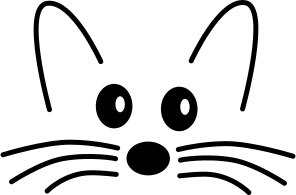
\includegraphics[width=1.4em]{squeak-logo}}}
\newcommand{\dothis}[1]{%
	\medskip
	\noindent\dothisicon
	\ifx#1\empty\else\quad\emph{#1}\fi
	\par\smallskip\nopagebreak}
% NB: To use this in an individual chapter, you must set:
%\graphicspath{{figures/} {../figures/}}
% at the head of the chapter.  Don't forget the final /
%=============================================================
%:Reader hints (hint)
%
% Indicates a non-obvious consequence 
\newcommand{\hint}[1]{\vspace{1ex}\noindent\fbox{\textsc{Astuce}} \emph{#1}}
%=================================================================
% graphics for Morphic handles
\newcommand{\grabHandle}{\raisebox{-0.2ex}{
\includegraphics[width=1em]{blackHandle}}}
\newcommand{\moveHandle}{\raisebox{-0.2ex}{
\includegraphics[width=1em]{moveHandle}}}
\newcommand{\debugHandle}{\raisebox{-0.2ex}{
\includegraphics[width=1em]{debugHandle}}}
% squeak-fr (added for Morphic handles)
\newcommand{\rotateHandle}{\raisebox{-0.2ex}{
\includegraphics[width=1em]{rotateHandle}}}
\newcommand{\viewerHandle}{\raisebox{-0.2ex}{
\includegraphics[width=1em]{viewerHandle}}}
% squeak-fr (add cloverHandle to use \clover in QuickTour.tex as alias
% todo 

%=============================================================
%:Highlighting Important stuff (doublebox)
%
% From Seaside book ...
\newsavebox{\SavedText}
\newlength{\InnerBoxRule}\setlength{\InnerBoxRule}{.75\fboxrule}
\newlength{\OuterBoxRule}\setlength{\OuterBoxRule}{1.5\fboxrule}
\newlength{\BoxSeparation}\setlength{\BoxSeparation}{1.5\fboxrule}
\addtolength{\BoxSeparation}{.5pt}
\newlength{\SaveBoxSep}\setlength{\SaveBoxSep}{2\fboxsep}
%
\newenvironment{doublebox}{\begin{lrbox}{\SavedText}
    \begin{minipage}{.75\textwidth}}
    {\end{minipage}\end{lrbox}\begin{center}
    \setlength{\fboxsep}{\BoxSeparation}\setlength{\fboxrule}{\OuterBoxRule}
    \fbox{\setlength{\fboxsep}{\SaveBoxSep}\setlength{\fboxrule}{\InnerBoxRule}%
      \fbox{\usebox{\SavedText}}}
  \end{center}}
% Use this:
%\newcommand{\important}[1]{\begin{doublebox}#1\end{doublebox}}


\newcommand{\important}[1]{
\noindent\rule{\textwidth}{2pt}\par
\textbf{Important!} #1 \par
\noindent\rule{\textwidth}{2pt}}

\newcommand{\note}[1]{
\noindent\rule{\textwidth}{2pt}\par
\noindent\textbf{Note} #1\par
\noindent\rule{\textwidth}{2pt}}

%=============================================================
%:Section depth
\setcounter{secnumdepth}{2}
%% for this to happen start the file with
%\ifx\wholebook\relax\else
%% $Author$ Martial
% $Date$ Wed Oct 10 13:34:55 CEST 2007
% $Revision$ source: SBE 12715 
% Last Changed Date: 2007-10-08 21:32:45 +0200 (Mon, 08 Oct 2007)
%=============================================================
% NB: documentclass must be set in main document.
% Allows book to be generated in multiple formats.
%=============================================================
%:Packages
%\usepackage[french]{babel}
\usepackage[T1]{fontenc}  %%%%%% really important to get the code directly in the text!
\usepackage{lmodern}
%\usepackage[scaled=0.85]{bookmanx} % needs another scale factor if used with \renewcommand{\sfdefault}{cmbr}
\usepackage{palatino}
%\usepackage[sc]{mathpazo}
%\linespread{1.05}
\usepackage[scaled=0.85]{helvet}
\usepackage{microtype}
\usepackage{graphicx}
\usepackage{theorem}
\usepackage[utf8]{inputenc}
% ON: pdfsync breaks the use of p{width} for tabular columns!
\ifdefined\usepdfsync\usepackage{pdfsync}\fi % Requires texlive 2007
%=============================================================
%:More packages
%Stef should check which ones are used!
%\usepackage{picinpar}
%\usepackage{layout}
%\usepackage{color}
%\definecolor{stefgris}{rgb}{0.85,0.85,0.85}
%\usepackage{enum}
%\usepackage{a4wide}
% \usepackage{fancyhdr}
\usepackage{ifthen}
\usepackage{float}
\usepackage{longtable}
\usepackage{makeidx}
\usepackage[nottoc]{tocbibind}
\usepackage{multicol}
\usepackage{booktabs}	% book-style tables
\usepackage{topcapt}	% enables \topcaption
\usepackage{multirow}
\usepackage{tabularx}
%\usepackage[bottom]{footmisc}
\usepackage{xspace}
\usepackage{alltt}
\usepackage{amssymb,textcomp}
\usepackage[usenames,dvipsnames]{color}
\usepackage{colortbl}
\usepackage[hang]{subfigure}\makeatletter\def\p@subfigure{\thefigure\,}\makeatother
\usepackage{rotating}
\usepackage{enumitem}	% apb: allows more control over tags in enumerations
\usepackage{verbatim}     % for comment environment
\usepackage{varioref}	% for page references that work
\labelformat{footnote}{\thechapter--#1} % to distinguish citations from jurabib
\usepackage{needspace}
\usepackage{isodateo} % enable \isodate
\usepackage[newparttoc]{titlesec}
\usepackage{titletoc}
\usepackage{eurosym}
\usepackage{wrapfig}

\usepackage[
	super,
	citefull=first,
	authorformat={allreversed,and},
	titleformat={commasep,italic}
]{jurabib} % citations as footnotes
\usepackage[
	colorlinks=true,
	linkcolor=black,
	urlcolor=black,
	citecolor=black
]{hyperref}   % should come last

%=============================================================
%:URL style
\makeatletter

\def\url@leostyle{%
  \@ifundefined{selectfont}{\def\UrlFont{\sf}}{\def\UrlFont{\sffamily}}}
% ajouter par Martial pour \traduit (met une dague dans les \doublebox
\def\thempfootnote{\fnsymbol{mpfootnote}}

\makeatother
% Now actually use the newly defined style.
\urlstyle{leo}
%=============================================================
%:Booleans
\newboolean{lulu}
\setboolean{lulu}{false}
\newcommand{\ifluluelse}[2]{\ifthenelse{\boolean{lulu}}{#1}{#2}}
%=============================================================
%:Names
\newcommand{\SUnit}{SUnit\xspace}
\newcommand{\sunit}{SUnit\xspace}
\newcommand{\xUnit}{$x$Unit\xspace}
\newcommand{\JUnit}{JUnit\xspace}
%\newcommand{\XP}{eXtreme Programming\xspace}
\newcommand{\st}{Smalltalk\xspace}
\newcommand{\Squeak}{Squeak\xspace}
\newcommand{\sq}{Squeak\xspace}
\newcommand{\sqmap}{SqueakMap\xspace}
\newcommand{\squeak}{Squeak\xspace}
%\newcommand{\sbe}{\url{scg.unibe.ch/SBE}\xspace}
%\newcommand{\sbe}{\url{squeakbyexample.org}\xspace}
\newcommand{\sbe}{\url{SqueakByExample.org}\xspace}
% squeak-fr: adresse de la version francaise
\newcommand{\spe}{\url{SqueakByExample.org/fr}\xspace}
\newcommand{\sba}{\url{SquareBracketAssociates.org}\xspace}

% squeak-fr: ajout de la \squeakdev pour eviter les problemes de
% changements d'url rencontres dans la VO:
\newcommand{\squeakdev}{\url{www.squeaksource.com/ImageForDevelopers}\xspace} %ou
%\newcommand{\squeakdev}{\url{squeak.ofset.org/squeak-dev}\xspace}

%=============================================================
%:Editorial comment macros
\newcommand{\nnbb}[2]{
    \fbox{\bfseries\sffamily\scriptsize#1}
    {\sf\small$\blacktriangleright$\textit{#2}$\blacktriangleleft$}
   }
\newcommand{\ab}[1]{\nnbb{Andrew}{#1}}
\newcommand{\sd}[1]{\nnbb{St\'{e}f}{#1}}
\newcommand{\md}[1]{\nnbb{Marcus}{#1}}
\newcommand{\on}[1]{\nnbb{Oscar}{#1}}
\newcommand{\damien}[1]{\nnbb{Damien}{#1}}
\newcommand{\lr}[1]{\nnbb{Lukas}{#1}}
\newcommand{\orla}[1]{\nnbb{Orla}{#1}}
%\newcommand{\here}{\nnbb{CONTINUE}{HERE}}
\newcommand{\here}{\nnbb{CONTINUE}{ICI}}

%=============================================================
%:Abbreviation macros
\newcommand{\ie}{\emph{c-\`a-d.}\xspace}
\newcommand{\cad}{\emph{c-\`a-d.}\xspace}
%\newcommand{\eg}{\emph{e.g.},\xspace}
\newcommand{\eg}{\emph{par ex.},\xspace}
\newcommand{\parex}{\emph{par ex.},\xspace}
\newcommand{\etc}{etc\xspace}
%=============================================================
%:Cross reference macros

% [squeak-fr] martial: remarquez les articles devant les noms
\newcommand{\charef}[1]{le chapitre~\ref{cha:#1}\xspace}
% note de martial: utilise dans chapitre Syntax.tex: a redefinir
\newcommand{\charefs}[2]{les chapitres~\ref{cha:#1} et \ref{cha:#2}\xspace}
\newcommand{\secref}[1]{la section~\ref{sec:#1}\xspace}
\newcommand{\figref}[1]{la figure~\ref{fig:#1}\xspace}
\newcommand{\Figref}[1]{La figure~\ref{fig:#1}\xspace}
\newcommand{\appref}[1]{l'annexe~\ref{app:#1}\xspace}
\newcommand{\tabref}[1]{la table~\ref{tab:#1}\xspace}
% defini pour le chapitre Messages.tex
\newcommand{\Tabref}[1]{La table~\ref{tab:#1}\xspace}

% APB: I removed trailing \xspace commands from these macros because
% \xspace mostly doesn't work.  If you want a space after your
% references, type one!
% ON: xspace has always worked just fine for me!  Please leave them in.
%
\newcommand{\ruleref}[1]{\ref{rule:#1}\xspace}
%
\newcommand{\egref}[1]{exemple~\ref{eg:#1}\xspace}
\newcommand{\Egref}[1]{Exemple~\ref{eg:#1}\xspace}
%
\newcommand{\scrref}[1]{script~\ref{scr:#1}\xspace}
\newcommand{\Scrref}[1]{Script~\ref{scr:#1}\xspace}
% t = the
\newcommand{\tscrref}[1]{le script~\ref{scr:#1}\xspace}
\newcommand{\Tscrref}[1]{Le script~\ref{scr:#1}\xspace}
%
\newcommand{\mthref}[1]{m\'ethode~\ref{mth:#1}\xspace}
\newcommand{\mthsref}[1]{m\'ethodes~\ref{mth:#1}\xspace}
\newcommand{\Mthref}[1]{M\'ethode~\ref{mth:#1}\xspace}
\newcommand{\tmthref}[1]{la m\'ethode~\ref{mth:#1}\xspace}
\newcommand{\Tmthref}[1]{La m\'ethode~\ref{mth:#1}\xspace}
%
\newcommand{\clsref}[1]{classe~\ref{cls:#1}\xspace}
\newcommand{\tclsref}[1]{la classe~\ref{cls:#1}\xspace}
\newcommand{\Tclsref}[1]{La classe~\ref{cls:#1}\xspace}
%=============================================================
%:Menu item macro
% for menu items, so we can change our minds on how to print them! (apb)
\definecolor{lightgray}{gray}{0.89}
\newcommand{\menu}[1]{{%
	\setlength{\fboxsep}{0pt}%
	\colorbox{lightgray}{{{\upshape\sffamily\strut \,#1\,}}}}}
% \newcommand{\menu}[1]{{%
% 	\fontfamily{lmr}\selectfont
% 	\upshape\textlangle{\sffamily #1}\textrangle}}
% For submenu items:
\newcommand{\go}{\,$\triangleright$\,}
% \newcommand{\go}{\,$\blacktriangleright$\,}
% For keyboard shortcuts:
%\newcommand{\short}[1]{\mbox{$\langle${\sc CMD}$\rangle$-#1}\xspace}
\newcommand{\short}[1]{\mbox{{\sc cmd}\hspace{0.08em}--\hspace{0.09em}#1}\xspace}
% For buttons:
\newcommand{\button}[1]{{%
	\setlength{\fboxsep}{0pt}%
	\fbox{{\upshape\sffamily\strut \,#1\,}}}}
\newcommand{\toolsflap}{l'onglet \textit{Tools}\xspace}
%=============================================================
%:Reader cues (do this)
%
% Indicate something the reader should try out.
\newcommand{\dothisicon}{\raisebox{-.5ex}{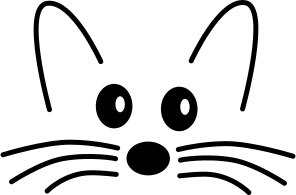
\includegraphics[width=1.4em]{squeak-logo}}}
\newcommand{\dothis}[1]{%
	\medskip
	\noindent\dothisicon
	\ifx#1\empty\else\quad\emph{#1}\fi
	\par\smallskip\nopagebreak}
% NB: To use this in an individual chapter, you must set:
%\graphicspath{{figures/} {../figures/}}
% at the head of the chapter.  Don't forget the final /
%=============================================================
%:Reader hints (hint)
%
% Indicates a non-obvious consequence 
\newcommand{\hint}[1]{\vspace{1ex}\noindent\fbox{\textsc{Astuce}} \emph{#1}}
%=================================================================
% graphics for Morphic handles
\newcommand{\grabHandle}{\raisebox{-0.2ex}{
\includegraphics[width=1em]{blackHandle}}}
\newcommand{\moveHandle}{\raisebox{-0.2ex}{
\includegraphics[width=1em]{moveHandle}}}
\newcommand{\debugHandle}{\raisebox{-0.2ex}{
\includegraphics[width=1em]{debugHandle}}}
% squeak-fr (added for Morphic handles)
\newcommand{\rotateHandle}{\raisebox{-0.2ex}{
\includegraphics[width=1em]{rotateHandle}}}
\newcommand{\viewerHandle}{\raisebox{-0.2ex}{
\includegraphics[width=1em]{viewerHandle}}}
% squeak-fr (add cloverHandle to use \clover in QuickTour.tex as alias
% todo 

%=============================================================
%:Highlighting Important stuff (doublebox)
%
% From Seaside book ...
\newsavebox{\SavedText}
\newlength{\InnerBoxRule}\setlength{\InnerBoxRule}{.75\fboxrule}
\newlength{\OuterBoxRule}\setlength{\OuterBoxRule}{1.5\fboxrule}
\newlength{\BoxSeparation}\setlength{\BoxSeparation}{1.5\fboxrule}
\addtolength{\BoxSeparation}{.5pt}
\newlength{\SaveBoxSep}\setlength{\SaveBoxSep}{2\fboxsep}
%
\newenvironment{doublebox}{\begin{lrbox}{\SavedText}
    \begin{minipage}{.75\textwidth}}
    {\end{minipage}\end{lrbox}\begin{center}
    \setlength{\fboxsep}{\BoxSeparation}\setlength{\fboxrule}{\OuterBoxRule}
    \fbox{\setlength{\fboxsep}{\SaveBoxSep}\setlength{\fboxrule}{\InnerBoxRule}%
      \fbox{\usebox{\SavedText}}}
  \end{center}}
% Use this:
%\newcommand{\important}[1]{\begin{doublebox}#1\end{doublebox}}


\newcommand{\important}[1]{
\noindent\rule{\textwidth}{2pt}\par
\textbf{Important!} #1 \par
\noindent\rule{\textwidth}{2pt}}

\newcommand{\note}[1]{
\noindent\rule{\textwidth}{2pt}\par
\noindent\textbf{Note} #1\par
\noindent\rule{\textwidth}{2pt}}

%=============================================================
%:Section depth
\setcounter{secnumdepth}{2}
%% for this to happen start the file with
%\ifx\wholebook\relax\else
%% $Author$ Martial
% $Date$ Wed Oct 10 13:34:55 CEST 2007
% $Revision$ source: SBE 12715 
% Last Changed Date: 2007-10-08 21:32:45 +0200 (Mon, 08 Oct 2007)
%=============================================================
% NB: documentclass must be set in main document.
% Allows book to be generated in multiple formats.
%=============================================================
%:Packages
%\usepackage[french]{babel}
\usepackage[T1]{fontenc}  %%%%%% really important to get the code directly in the text!
\usepackage{lmodern}
%\usepackage[scaled=0.85]{bookmanx} % needs another scale factor if used with \renewcommand{\sfdefault}{cmbr}
\usepackage{palatino}
%\usepackage[sc]{mathpazo}
%\linespread{1.05}
\usepackage[scaled=0.85]{helvet}
\usepackage{microtype}
\usepackage{graphicx}
\usepackage{theorem}
\usepackage[utf8]{inputenc}
% ON: pdfsync breaks the use of p{width} for tabular columns!
\ifdefined\usepdfsync\usepackage{pdfsync}\fi % Requires texlive 2007
%=============================================================
%:More packages
%Stef should check which ones are used!
%\usepackage{picinpar}
%\usepackage{layout}
%\usepackage{color}
%\definecolor{stefgris}{rgb}{0.85,0.85,0.85}
%\usepackage{enum}
%\usepackage{a4wide}
% \usepackage{fancyhdr}
\usepackage{ifthen}
\usepackage{float}
\usepackage{longtable}
\usepackage{makeidx}
\usepackage[nottoc]{tocbibind}
\usepackage{multicol}
\usepackage{booktabs}	% book-style tables
\usepackage{topcapt}	% enables \topcaption
\usepackage{multirow}
\usepackage{tabularx}
%\usepackage[bottom]{footmisc}
\usepackage{xspace}
\usepackage{alltt}
\usepackage{amssymb,textcomp}
\usepackage[usenames,dvipsnames]{color}
\usepackage{colortbl}
\usepackage[hang]{subfigure}\makeatletter\def\p@subfigure{\thefigure\,}\makeatother
\usepackage{rotating}
\usepackage{enumitem}	% apb: allows more control over tags in enumerations
\usepackage{verbatim}     % for comment environment
\usepackage{varioref}	% for page references that work
\labelformat{footnote}{\thechapter--#1} % to distinguish citations from jurabib
\usepackage{needspace}
\usepackage{isodateo} % enable \isodate
\usepackage[newparttoc]{titlesec}
\usepackage{titletoc}
\usepackage{eurosym}
\usepackage{wrapfig}

\usepackage[
	super,
	citefull=first,
	authorformat={allreversed,and},
	titleformat={commasep,italic}
]{jurabib} % citations as footnotes
\usepackage[
	colorlinks=true,
	linkcolor=black,
	urlcolor=black,
	citecolor=black
]{hyperref}   % should come last

%=============================================================
%:URL style
\makeatletter

\def\url@leostyle{%
  \@ifundefined{selectfont}{\def\UrlFont{\sf}}{\def\UrlFont{\sffamily}}}
% ajouter par Martial pour \traduit (met une dague dans les \doublebox
\def\thempfootnote{\fnsymbol{mpfootnote}}

\makeatother
% Now actually use the newly defined style.
\urlstyle{leo}
%=============================================================
%:Booleans
\newboolean{lulu}
\setboolean{lulu}{false}
\newcommand{\ifluluelse}[2]{\ifthenelse{\boolean{lulu}}{#1}{#2}}
%=============================================================
%:Names
\newcommand{\SUnit}{SUnit\xspace}
\newcommand{\sunit}{SUnit\xspace}
\newcommand{\xUnit}{$x$Unit\xspace}
\newcommand{\JUnit}{JUnit\xspace}
%\newcommand{\XP}{eXtreme Programming\xspace}
\newcommand{\st}{Smalltalk\xspace}
\newcommand{\Squeak}{Squeak\xspace}
\newcommand{\sq}{Squeak\xspace}
\newcommand{\sqmap}{SqueakMap\xspace}
\newcommand{\squeak}{Squeak\xspace}
%\newcommand{\sbe}{\url{scg.unibe.ch/SBE}\xspace}
%\newcommand{\sbe}{\url{squeakbyexample.org}\xspace}
\newcommand{\sbe}{\url{SqueakByExample.org}\xspace}
% squeak-fr: adresse de la version francaise
\newcommand{\spe}{\url{SqueakByExample.org/fr}\xspace}
\newcommand{\sba}{\url{SquareBracketAssociates.org}\xspace}

% squeak-fr: ajout de la \squeakdev pour eviter les problemes de
% changements d'url rencontres dans la VO:
\newcommand{\squeakdev}{\url{www.squeaksource.com/ImageForDevelopers}\xspace} %ou
%\newcommand{\squeakdev}{\url{squeak.ofset.org/squeak-dev}\xspace}

%=============================================================
%:Editorial comment macros
\newcommand{\nnbb}[2]{
    \fbox{\bfseries\sffamily\scriptsize#1}
    {\sf\small$\blacktriangleright$\textit{#2}$\blacktriangleleft$}
   }
\newcommand{\ab}[1]{\nnbb{Andrew}{#1}}
\newcommand{\sd}[1]{\nnbb{St\'{e}f}{#1}}
\newcommand{\md}[1]{\nnbb{Marcus}{#1}}
\newcommand{\on}[1]{\nnbb{Oscar}{#1}}
\newcommand{\damien}[1]{\nnbb{Damien}{#1}}
\newcommand{\lr}[1]{\nnbb{Lukas}{#1}}
\newcommand{\orla}[1]{\nnbb{Orla}{#1}}
%\newcommand{\here}{\nnbb{CONTINUE}{HERE}}
\newcommand{\here}{\nnbb{CONTINUE}{ICI}}

%=============================================================
%:Abbreviation macros
\newcommand{\ie}{\emph{c-\`a-d.}\xspace}
\newcommand{\cad}{\emph{c-\`a-d.}\xspace}
%\newcommand{\eg}{\emph{e.g.},\xspace}
\newcommand{\eg}{\emph{par ex.},\xspace}
\newcommand{\parex}{\emph{par ex.},\xspace}
\newcommand{\etc}{etc\xspace}
%=============================================================
%:Cross reference macros

% [squeak-fr] martial: remarquez les articles devant les noms
\newcommand{\charef}[1]{le chapitre~\ref{cha:#1}\xspace}
% note de martial: utilise dans chapitre Syntax.tex: a redefinir
\newcommand{\charefs}[2]{les chapitres~\ref{cha:#1} et \ref{cha:#2}\xspace}
\newcommand{\secref}[1]{la section~\ref{sec:#1}\xspace}
\newcommand{\figref}[1]{la figure~\ref{fig:#1}\xspace}
\newcommand{\Figref}[1]{La figure~\ref{fig:#1}\xspace}
\newcommand{\appref}[1]{l'annexe~\ref{app:#1}\xspace}
\newcommand{\tabref}[1]{la table~\ref{tab:#1}\xspace}
% defini pour le chapitre Messages.tex
\newcommand{\Tabref}[1]{La table~\ref{tab:#1}\xspace}

% APB: I removed trailing \xspace commands from these macros because
% \xspace mostly doesn't work.  If you want a space after your
% references, type one!
% ON: xspace has always worked just fine for me!  Please leave them in.
%
\newcommand{\ruleref}[1]{\ref{rule:#1}\xspace}
%
\newcommand{\egref}[1]{exemple~\ref{eg:#1}\xspace}
\newcommand{\Egref}[1]{Exemple~\ref{eg:#1}\xspace}
%
\newcommand{\scrref}[1]{script~\ref{scr:#1}\xspace}
\newcommand{\Scrref}[1]{Script~\ref{scr:#1}\xspace}
% t = the
\newcommand{\tscrref}[1]{le script~\ref{scr:#1}\xspace}
\newcommand{\Tscrref}[1]{Le script~\ref{scr:#1}\xspace}
%
\newcommand{\mthref}[1]{m\'ethode~\ref{mth:#1}\xspace}
\newcommand{\mthsref}[1]{m\'ethodes~\ref{mth:#1}\xspace}
\newcommand{\Mthref}[1]{M\'ethode~\ref{mth:#1}\xspace}
\newcommand{\tmthref}[1]{la m\'ethode~\ref{mth:#1}\xspace}
\newcommand{\Tmthref}[1]{La m\'ethode~\ref{mth:#1}\xspace}
%
\newcommand{\clsref}[1]{classe~\ref{cls:#1}\xspace}
\newcommand{\tclsref}[1]{la classe~\ref{cls:#1}\xspace}
\newcommand{\Tclsref}[1]{La classe~\ref{cls:#1}\xspace}
%=============================================================
%:Menu item macro
% for menu items, so we can change our minds on how to print them! (apb)
\definecolor{lightgray}{gray}{0.89}
\newcommand{\menu}[1]{{%
	\setlength{\fboxsep}{0pt}%
	\colorbox{lightgray}{{{\upshape\sffamily\strut \,#1\,}}}}}
% \newcommand{\menu}[1]{{%
% 	\fontfamily{lmr}\selectfont
% 	\upshape\textlangle{\sffamily #1}\textrangle}}
% For submenu items:
\newcommand{\go}{\,$\triangleright$\,}
% \newcommand{\go}{\,$\blacktriangleright$\,}
% For keyboard shortcuts:
%\newcommand{\short}[1]{\mbox{$\langle${\sc CMD}$\rangle$-#1}\xspace}
\newcommand{\short}[1]{\mbox{{\sc cmd}\hspace{0.08em}--\hspace{0.09em}#1}\xspace}
% For buttons:
\newcommand{\button}[1]{{%
	\setlength{\fboxsep}{0pt}%
	\fbox{{\upshape\sffamily\strut \,#1\,}}}}
\newcommand{\toolsflap}{l'onglet \textit{Tools}\xspace}
%=============================================================
%:Reader cues (do this)
%
% Indicate something the reader should try out.
\newcommand{\dothisicon}{\raisebox{-.5ex}{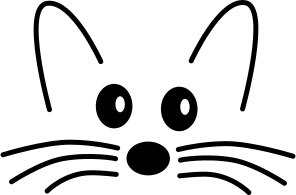
\includegraphics[width=1.4em]{squeak-logo}}}
\newcommand{\dothis}[1]{%
	\medskip
	\noindent\dothisicon
	\ifx#1\empty\else\quad\emph{#1}\fi
	\par\smallskip\nopagebreak}
% NB: To use this in an individual chapter, you must set:
%\graphicspath{{figures/} {../figures/}}
% at the head of the chapter.  Don't forget the final /
%=============================================================
%:Reader hints (hint)
%
% Indicates a non-obvious consequence 
\newcommand{\hint}[1]{\vspace{1ex}\noindent\fbox{\textsc{Astuce}} \emph{#1}}
%=================================================================
% graphics for Morphic handles
\newcommand{\grabHandle}{\raisebox{-0.2ex}{
\includegraphics[width=1em]{blackHandle}}}
\newcommand{\moveHandle}{\raisebox{-0.2ex}{\includegraphics[width=1em]{moveHandle}}}
\newcommand{\debugHandle}{\raisebox{-0.2ex}{\includegraphics[width=1em]{debugHandle}}}
% squeak-fr (added for Morphic handles)
\newcommand{\rotateHandle}{\raisebox{-0.2ex}{\includegraphics[width=1em]{rotateHandle}}}
\newcommand{\viewerHandle}{\raisebox{-0.2ex}{\includegraphics[width=1em]{viewerHandle}}}
% squeak-fr (add cloverHandle to use \clover in QuickTour.tex as alias
% todo 

%=============================================================
%:Highlighting Important stuff (doublebox)
%
% From Seaside book ...
\newsavebox{\SavedText}
\newlength{\InnerBoxRule}\setlength{\InnerBoxRule}{.75\fboxrule}
\newlength{\OuterBoxRule}\setlength{\OuterBoxRule}{1.5\fboxrule}
\newlength{\BoxSeparation}\setlength{\BoxSeparation}{1.5\fboxrule}
\addtolength{\BoxSeparation}{.5pt}
\newlength{\SaveBoxSep}\setlength{\SaveBoxSep}{2\fboxsep}
%
\newenvironment{doublebox}{\begin{lrbox}{\SavedText}
    \begin{minipage}{.75\textwidth}}
    {\end{minipage}\end{lrbox}\begin{center}
    \setlength{\fboxsep}{\BoxSeparation}\setlength{\fboxrule}{\OuterBoxRule}
    \fbox{\setlength{\fboxsep}{\SaveBoxSep}\setlength{\fboxrule}{\InnerBoxRule}%
      \fbox{\usebox{\SavedText}}}
  \end{center}}
% Use this:
%\newcommand{\important}[1]{\begin{doublebox}#1\end{doublebox}}


\newcommand{\important}[1]{
\noindent\rule{\textwidth}{2pt}\par
\textbf{Important!} #1 \par
\noindent\rule{\textwidth}{2pt}}

\newcommand{\note}[1]{
\noindent\rule{\textwidth}{2pt}\par
\noindent\textbf{Note} #1\par
\noindent\rule{\textwidth}{2pt}}

%=============================================================
%:Section depth
\setcounter{secnumdepth}{2}
%% for this to happen start the file with
%\ifx\wholebook\relax\else
%\input{../common.tex}
%\begin{document}
%\fi
% and terminate by
% \ifx\wholebook\relax\else\end{document}\fi

\DeclareGraphicsExtensions{.pdf, .jpg, .png}
%=============================================================
%:PDF setup
\hypersetup{
%   a4paper,
%   pdfstartview=FitV,
%   colorlinks,
%   linkcolor=darkblue,
%   citecolor=darkblue,
%   pdftitle={Squeak by Example},
pdftitle={Squeak par l'exemple},
   pdfauthor={Andrew Black, St\'ephane Ducasse,	Oscar Nierstrasz,
Damien Pollet},
   pdfkeywords={Smalltalk, Squeak, Programmation Orient\'ee Objet},
pdfsubject={Informatique, Computer Science}
}
%=============================================================
%:Page layout and appearance
%
% \renewcommand{\headrulewidth}{0pt}
\renewcommand{\chaptermark}[1]{\markboth{#1}{}}
\renewcommand{\sectionmark}[1]{\markright{\thesection\ #1}}
\renewpagestyle{plain}[\small\itshape]{%
	\setheadrule{0pt}%
	\sethead[][][]{}{}{}%
	\setfoot[][][]{}{}{}}
\renewpagestyle{headings}[\small\itshape]{%
	\setheadrule{0pt}%
	\setmarks{chapter}{section}%
	\sethead[\thepage][][\chaptertitle]{\sectiontitle}{}{\thepage}%
	\setfoot[][][]{}{}{}}
% pagestyle for tableofcontents + index (martial: 2008/04/23)
\newpagestyle{newheadings}[\small\itshape]{%
	\setheadrule{0pt}%
	\setmarks{chapter}{section}%
	\sethead[\thepage][][\chaptertitle]{\chaptertitle}{}{\thepage}%
	\setfoot[][][]{}{}{}}
%=============================================================
%:Title section setup and TOC numbering depth
\setcounter{secnumdepth}{1}
\setcounter{tocdepth}{1}
\titleformat{\part}[display]{\centering}{\huge\partname\ \thepart}{1em}{\Huge\textbf}[]
\titleformat{\chapter}[display]{}{\huge\chaptertitlename\ \thechapter}{1em}{\Huge\raggedright\textbf}[]
\titlecontents{part}[3pc]{%
		\pagebreak[2]\addvspace{1em plus.4em minus.2em}%
		\leavevmode\large\bfseries}
	{\contentslabel{3pc}}{\hspace*{-3pc}}
	{}[\nopagebreak]
\titlecontents{chapter}[3pc]{%
		\pagebreak[0]\addvspace{1em plus.2em minus.2em}%
		\leavevmode\bfseries}
	{\contentslabel{3pc}}{}
	{\hfill\contentspage}[\nopagebreak]
\dottedcontents{section}[3pc]{}{3pc}{1pc}
\dottedcontents{subsection}[3pc]{}{0pc}{1pc}
% \dottedcontents{subsection}[4.5em]{}{0pt}{1pc}
% Make \cleardoublepage insert really blank pages http://www.tex.ac.uk/cgi-bin/texfaq2html?label=reallyblank
\let\origdoublepage\cleardoublepage
\newcommand{\clearemptydoublepage}{%
  \clearpage
  {\pagestyle{empty}\origdoublepage}}
\let\cleardoublepage\clearemptydoublepage % see http://www.tex.ac.uk/cgi-bin/texfaq2html?label=patch
%=============================================================
%:FAQ macros (for FAQ chapter)
\newtheorem{faq}{FAQ}
\newcommand{\answer}{\paragraph{R\'eponse}\ }
%=============================================================
%:Listings package configuration
\usepackage{listings}
\newcommand{\caret}{\makebox{\raisebox{0.4ex}{\footnotesize{$\wedge$}}}}
\lstdefinelanguage{Smalltalk}{
%  morekeywords={self,super,true,false,nil,thisContext}, % This is overkill
  morestring=[d]',
  morecomment=[s]{"}{"},
  alsoletter={\#:},
  escapechar={!},
  escapebegin=\itshape, % comment-like by default (Martial 11/2007)
  literate=
    {BANG}{!}1
    {UNDERSCORE}{\_}1
    {\\st}{Smalltalk}9 % convenience -- in case \st occurs in code
    % {'}{{\textquotesingle}}1 % replaced by upquote=true in \lstset
    {_}{{$\leftarrow$}}1
    {>>>}{{\sep}}1
    {^}{{$\uparrow$}}1
    {~}{{$\sim$}}1
    {-}{{\sf -\hspace{-0.13em}-}}1  % the goal is to make - the same width as +
    {+}{\raisebox{0.08ex}{+}}1		% and to raise + off the baseline to match -
    {-->}{{\quad$\longrightarrow$\quad}}3
	, % Don't forget the comma at the end!
  tabsize=4
}[keywords,comments,strings]
% ajout pour les échappements dans les codes
% indispensable pour mettre le code en emphase (cf. Model.tex) 
\newcommand{\codeify}[1]{\NoAutoSpaceBeforeFDP#1\AutoSpaceBeforeFDP}
\newcommand{\normcomment}[1]{\emph{#1}} %cf. Streams
\newcommand{\normcode}[1]{\emph{\codeify{#1}}} %cf. Streams
\newcommand{\emcode}[1]{\textbf{\normcode{#1}}} % Martial 11/2007
\lstset{language=Smalltalk,
	basicstyle=\sffamily,
	keywordstyle=\color{black}\bfseries,
	% stringstyle=\ttfamily, % Ugly! do we really want this? -- on
	%commentstyle=\itshape,
	mathescape=true,
	showstringspaces=false,
	keepspaces=true,
	breaklines=true,
	breakautoindent=true,
	lineskip={-1pt}, % Ugly hack
	upquote=true, % straight quote; requires textcomp package
	columns=fullflexible} % no fixed width fonts
% In-line code (literal)
% Normally use this for all in-line code:
\newcommand{\ct}{\lstinline[mathescape=false,basicstyle={\sffamily\upshape}]}
% apb 2007.8.28 added the \upshape declaration to avoid getting italicized code in \dothis{ } sections.
% In-line code (latex enabled)
% Use this only in special situations where \ct does not work
% (within section headings ...):

% [squeak-fr] Modification de \lct suivant les indications de Martial Boniou
\newcommand{\lct}[1]{\textsf{\textup{\NoAutoSpaceBeforeFDP #1
\AutoSpaceBeforeFDP}}} %\xspace

% Use these for system categories and protocols:
\newcommand{\scat}[1]{\emph{\textsf{#1}}\xspace}
\newcommand{\pkg}[1]{\emph{\textsf{#1}}\xspace}
\newcommand{\prot}[1]{\emph{\textsf{#1}}\xspace}
% Code environments
% NB: the arg is for tests
% Only code and example environments may be tests
\lstnewenvironment{code}[1]{%
	\lstset{%
		frame=lines,
		mathescape=false
	}
}{}
\def\ignoredollar#1{}
%=============================================================
%:Code environments (method, script ...)
% NB: the third arg is for tests
% Only code and example environments may be tests
\lstnewenvironment{example}[3][defaultlabel]{%
	\renewcommand{\lstlistingname}{Exemple}%
	\lstset{
		frame=lines,
		mathescape=false,
		caption={\emph{#2}},
		label={eg:#1}
	}
}{}
\lstnewenvironment{script}[2][defaultlabel]{%
\renewcommand{\lstlistingname}{Script}%
	\lstset{
		frame=lines,
		mathescape=false,
		name={Script},
		caption={\emph{#2}},
		label={scr:#1}
	}
}{}
%I could not find a way yo get the Experiment #numb followed by the caption in a black box
%\colorbox{black}{\makebox[\textwidth]{  \color{white} {\large {\bfseries Experiment 3-1 (crear i moure un robot)}} }}
\lstnewenvironment{experiment}[2][defaultlabel]{%
%\noindent\rule{\textwidth}{2pt}\vspace{-0.8cm}
\renewcommand{\lstlistingname}{Experiment}%
	\lstset{
		frame=none,
		rulecolor=\color{black},
		mathescape=false,
		name={Experiment},
		caption={\emph{#2}},
		label={scr:#1}
	}
}{%\vspace{-0.5cm}\noindent\rule{\textwidth}{2pt}
}

\lstnewenvironment{method}[2][defaultlabel]{%
	\renewcommand{\lstlistingname}{Method}%
	\lstset{
		frame=lines,
		mathescape=false,
		name={M\'ethode},
		caption={\emph{#2}},
		label={mth:#1}
	}
}{}
\lstnewenvironment{methods}[2][defaultlabel]{% just for multiple methods at once
	\renewcommand{\lstlistingname}{Methods}%
	\lstset{
		frame=lines,
		mathescape=false,
		name={M\'ethode},
		caption={\emph{#2}},
		label={mth:#1}
	}
}{}
\lstnewenvironment{numMethod}[2][defaultlabel]{%
	\renewcommand{\lstlistingname}{Method}%
	\lstset{
		numbers=left,
		numberstyle={\tiny\sffamily},
		frame=lines,
		mathescape=false,
		name={M\'ethode},
		caption={\emph{#2}},
		label={mth:#1}
	}
}{}
% \lstnewenvironment{classdef}[2][defaultlabel]{%
% 	\renewcommand{\lstlistingname}{Classe}%
% 	\lstset{
% 		frame=lines,
% 		mathescape=false,
% 		name={Classe},
% 		caption={\emph{#2}},
% 		label={cls:#1}
% 	}
% }{}

%%%%%%%%%%%%%%%%%%%%%%%%%%%%%%%%%%%%%%%%%%%%%%%%%%%%%%%%%%%%%%%%%%%%%%%%%%%%%%%%%%%%%%%%%%%%%%%%%
%%From the original book latex template
%%%%%%%%%%%%%%%%%%%%%%%%%%%%%%%%%%%%%%%%%%%%%%%%%%%%%%%%%%%%%%%%%%%%%%%%%%%%%%%%%%%%%%%%%%%%%%%%%
\theoremstyle{break}
{\theorembodyfont{\rmfamily}\theoremstyle{break}
\newtheorem{privScript}{Script}[chapter]
%\newtheorem{privMethod}{Method}[chapter]
\newtheorem{privExercise}{Experiment}[chapter]}

% \theoremstyle{break}
% {\theorembodyfont{\rmfamily} \newtheorem{privMethod}{Method}[chapter]}

%class
\theoremstyle{break}
{\theorembodyfont{\rmfamily} \newtheorem{privClassDef}{Class}[chapter]}

%important
\theoremstyle{break}
{\theorembodyfont{\rmfamily} \newtheorem{privTemplate}{Important Messages}[chapter]}

% experiment
\newenvironment{exercise}
    {\begin{privExercise}\mbox{}\\}
    {\end{privExercise}}


%%% for figure
\newsavebox{\ScriptFigure}
\newlength{\ScriptWidth}
\newlength{\FigureWidth}

%%%%%%%%%%%%%%%%%%%%%%%%%%%%%%%%%%%%%%%%%%%%%%%%%%%%%%%%%%%%%%%%%%%%%%%%%%%%%%%%
\newenvironment{scriptfig}[3][0.6]
   {\setlength{\ScriptWidth}{\linewidth*\real{#1}}%
   \setlength{\FigureWidth}{\linewidth-(\linewidth*\real{#1})}%
   \savebox{\ScriptFigure}%
	{\parbox{\FigureWidth}{\includegraphics[width=0.98\FigureWidth]{#2}}}%
   \par\noindent\begin{minipage}{\linewidth}\hrule\vskip 0.2cm\begin{minipage}[c]{\ScriptWidth}%
   \begin{stefscript}[{\em #3}]\begin{alltt}\sffamily}
   {\end{alltt}\end{stefscript}\end{minipage}\hfill
   \usebox{\ScriptFigure}
   \vskip 1ex\hrule\end{minipage}\vskip 1ex\par}

%%%%%%%%%%%%%%%%%%%%%%%%%%%%%%%%%%%%%%%%%%%%%%%%%%%%%%%%%%%%%%%%%%%%%%%%%%%%%%%%
%% to be able to specify the complete set of values for includegraphics
%% may be will be changed but not the interface
\newenvironment{scriptfigwithsize}[3][0.6]
   {\setlength{\ScriptWidth}{\linewidth*\real{#1}}%
   \setlength{\FigureWidth}{\linewidth-(\linewidth*\real{#1})}%
   \savebox{\ScriptFigure}{\parbox{\FigureWidth}{\raggedleft{#2}}}%
   \par\noindent\begin{minipage}{\linewidth}\hrule\vskip 0.3cm\begin{minipage}[c]{\ScriptWidth}%
   \begin{stefscript}[{\em #3}]\begin{alltt}\sffamily}
   {\end{alltt}\end{stefscript}\end{minipage}\hfill
   \usebox{\ScriptFigure}
   \vskip 1ex\hrule\end{minipage}\vskip 1ex\par}

% \newenvironment{methodfig}[2][0.6]
%    {\setlength{\ScriptWidth}{\linewidth*\real{#1}}%
%    \setlength{\FigureWidth}{\linewidth-(\linewidth*\real{#1})}%
%    \savebox{\ScriptFigure}{\parbox{\FigureWidth}{\includegraphics[width=.98\FigureWidth]{#2}}}%
%    \par\noindent\rule{\linewidth}{1mm}
%    \\[-0.3cm]\noindent\rule{\linewidth}{0.1mm}
%    \noindent\begin{minipage}[c]{\ScriptWidth}\begin{privMethod}\begin{alltt}\sffamily}
%    {\end{alltt}\end{privMethod}\end{minipage}\hfill
%    \usebox{\ScriptFigure} \vskip 1ex\hrule\vskip 1ex\par}

% \newenvironment{method}
% {\par\noindent\begin{minipage}{\linewidth}\vspace{0.2cm}\begin{privMethod}\begin{nminipage}\vspace{-0.2cm}\rule{\linewidth}{1mm}\\[-0.6cm]\rule{\linewidth}{0.1mm}\end{nminipage}\hspace*{\scriptindent}\codesize\begin{nalltt}\vspace{-0.2cm}}
% {\end{nalltt}\normalsize\vspace{-0.1cm}\hrule\end{privMethod}\vspace{0.2cm}\end{minipage}}


% \newenvironment{classdef}
% {\par\noindent\begin{minipage}{\linewidth}\vspace{0.2cm}\begin{privClassDef}\begin{nminipage}\vspace{-0.2cm}\rule{\linewidth}{1mm}\\[-0.6cm]\rule{\linewidth}{0.1mm}\end{nminipage}\hspace*{\scriptindent}\codesize\begin{nalltt}\vspace{-0.2cm}}
% {\end{nalltt}\normalsize\vspace{-0.1cm}\hrule\end{privClassDef}\vspace{0.2cm}\end{minipage}}


% \newenvironment{template}
% {\par\noindent\begin{minipage}{\linewidth}\vspace{0.3cm}\begin{privTemplate}\begin{nminipage}\vspace{-0.4cm}\rule{\linewidth}{0.1mm}\end{nminipage}\hspace*{\scriptindent}\begin{nalltt}\vspace{-0.7cm}}
% {\end{nalltt}\vspace{-0.1cm}\hrule\end{privTemplate}\end{minipage}\vspace{0.3cm}}

\newenvironment{exofig}[2][0.7]
   {\setlength{\ScriptWidth}{\linewidth*\real{#1}}
   \setlength{\FigureWidth}{\linewidth-(\linewidth*\real{#1})}
   \savebox{\ScriptFigure}{\parbox{\FigureWidth}{\raggedleft{\includegraphics[width=.98\FigureWidth]{#2}}}}
   \par\noindent\begin{minipage}{\linewidth}\hrule\vskip 0.3cm\begin{minipage}[c]{\ScriptWidth}%
   \begin{privExercise}}
   {\end{privExercise}\end{minipage}\hfill
   \usebox{\ScriptFigure}
   \vskip 1ex\hrule\end{minipage}\vskip 1ex\par}

\newenvironment{exofigwithsize}[2][0.7]
   {\setlength{\ScriptWidth}{\linewidth*\real{#1}}
   \setlength{\FigureWidth}{\linewidth-(\linewidth*\real{#1})}
   \savebox{\ScriptFigure}{\parbox{\FigureWidth}{\raggedleft{#2}}}
   \par\noindent\begin{minipage}{\linewidth}\hrule\vskip 0.3cm\begin{minipage}[c]{\ScriptWidth}%
   \begin{privExercise}}
   {\end{privExercise}\end{minipage}\hfill\usebox{\ScriptFigure}
   \vskip 1ex\hrule\end{minipage}\vskip 1ex\par}

\newenvironment{exofigwithsizeandtitle}[3][0.7]
   {\setlength{\ScriptWidth}{\linewidth*\real{#1}}
   \setlength{\FigureWidth}{\linewidth-(\linewidth*\real{#1})}
   \savebox{\ScriptFigure}{\parbox{\FigureWidth}{\raggedleft{#2}}}
   \vskip 0.3cm\par\noindent\begin{minipage}{\linewidth}\hrule\vskip 0.1cm\begin{minipage}[c]{\ScriptWidth}%
   \begin{privExercise}[\em{#3}]}
   {\end{privExercise}\end{minipage}\hfill\usebox{\ScriptFigure}
   \vskip 1ex\hrule\end{minipage}\vskip 1ex\par}

\newenvironment{exofigwithtitle}[3][0.7]
   {\setlength{\ScriptWidth}{\linewidth*\real{#1}}
   \setlength{\FigureWidth}{\linewidth-(\linewidth*\real{#1})}
   \savebox{\ScriptFigure}{\parbox{\FigureWidth}{\raggedleft{\includegraphics[width=.98\FigureWidth]{#2}}}}
   \par\noindent\begin{minipage}{\linewidth}\hrule\vskip 0.3cm\begin{minipage}[c]{\ScriptWidth}%
   \begin{privExercise}[\em{#3}]}
   {\end{privExercise}\end{minipage}\hfill
   \usebox{\ScriptFigure}
   \vskip 1ex\hrule\end{minipage}\vskip 1ex\par}


\newenvironment{exonofigwithtitle}[3][0.7]
   {\setlength{\ScriptWidth}{\linewidth*\real{#1}}
   \setlength{\FigureWidth}{\linewidth-(\linewidth*\real{#1})}
   \savebox{\ScriptFigure}{\parbox{\FigureWidth}{\raggedleft{\includegraphics[width=.98\FigureWidth]{#2}}}}
   \par\noindent\begin{minipage}{\linewidth}\hrule\vskip 0.3cm\begin{minipage}[c]{\ScriptWidth}%
   \begin{privExercise}[\em{#3}]}
   {\end{privExercise}\end{minipage}\hfill
   \usebox{\ScriptFigure}
   \vskip 1ex\hrule\end{minipage}\vskip 1ex\par}

\newenvironment{exonofig}
   {\par\noindent\begin{minipage}[t]{\linewidth}\noindent\begin{privExercise}}
   {\end{privExercise}\end{minipage}\vspace{0.5cm}\par}

\newenvironment{exonofigtitle}[1]
   {\par\noindent\begin{minipage}[t]{\linewidth}\noindent\begin{privExercise}[\em{#1}]}
   {\end{privExercise}\end{minipage}\vspace{0.5cm}\par}
		
% \newenvironment{solfig}[3][0.5]
%    {\setlength{\ScriptWidth}{\linewidth*\real{#1}}
%    \setlength{\FigureWidth}{\linewidth-\linewidth*\real{#1}}
%    \savebox{\ScriptFigure}{\parbox{\FigureWidth}{\includegraphics[width=.9\linewidth]{#2}}}
%    \par\noindent\vskip 1ex\hrule\vskip 1ex\begin{minipage}[t]{\ScriptWidth}
%    {\bf Solution #3} \begin{alltt}\sffamily}
%    {\end{alltt}\end{minipage}\hfill
%    \usebox{\ScriptFigure}
%    \vskip 1ex\hrule\vskip 1ex\par}
% 
% \newenvironment{solnofig}[1]
%    {\par\noindent\vskip 1ex\hrule\vskip 1ex\begin{minipage}[t]{\ScriptWidth}
%    {\bf Solution #1} \begin{alltt}\sffamily}
%    {\end{alltt}\end{minipage}\hfill
%    \vskip 1ex\hrule\vskip 1ex\par}
% 
% \newenvironment{exoscript}[3][0.5]
%    {\setlength{\ScriptWidth}{\linewidth*\real{#1}}
%     \setlength{\FigureWidth}{\linewidth-\linewidth*\real{#1}}
%     \savebox{\ScriptFigure}{\begin{minipage}\begin{alltt}\sffamily#3\end{alltt}\end{minipage}}
%     \par\noindent\vskip 1ex\hrule\vskip 1ex\begin{minipage}[t]{\ScriptWidth}
%     \begin{privExercise}}
%     {\end{privExercise}\end{minipage}\hfill
%     \usebox{\ScriptFigure}
% \vskip 1ex\hrule\vskip 1ex\par}


%%%%%%%%%%%%%%%%%%%%%%%%%%%%%%%%%%%%%%%%%%%%%%%%%%%%%%%%%%%%%%%%
%% Define the indentation from which the code script starts
%\newlength{\scriptindent}
%\setlength{\scriptindent}{.3cm}
%%%%%%%%%%%%%%%%%%%%%%%%%%%%%%%%%%%%%%%%%%%%%%%%%%%%%%%%%%%%%%%%
%% Method presentation 
%\newlength{\methodindent}
%\newlength{\methodwordlength}
%\newlength{\aftermethod}
%\setlength{\methodindent}{0.2cm}
%\settowidth{\methodwordlength}{\ M\'ethode\ }

%%%%%%%%%%%%%%%%%%%%%%%%%%%%%%%%%%%%%%%%%%%%%%%%%%%%%%%%%%%%%%%%
\theoremstyle{break}
{\theorembodyfont{\rmfamily} \newtheorem{fonction}{Script}[chapter]}

\newsavebox{\fminibox}
\newlength{\fminilength}
% Fait un truc encadre
\newenvironment{fminipage}[1][\linewidth]
  {\setlength{\fminilength}{#1-2\fboxsep-2\fboxrule}
        \begin{lrbox}{\fminibox}\begin{minipage}{\fminilength}}
  { \end{minipage}\end{lrbox}\noindent\fbox{\usebox{\fminibox}}}

% Pareil mais pas encadre (a utiliser pour ne pas couper une fonction en 2)
\newenvironment{nminipage}[1][\linewidth]
  {\setlength{\fminilength}{#1}
        \begin{lrbox}{\fminibox}\begin{minipage}{\fminilength}}
  { \end{minipage}\end{lrbox}\noindent\mbox{\usebox{\fminibox}}}

% Un alltt encadre
\newenvironment{falltt}
  {\vspace*{0.3cm}\begin{fminipage}\begin{alltt}\ttfamily}
  {\end{alltt}\end{fminipage}\vspace*{0.3cm}}

% Un alltt pas encadre
\newenvironment{nalltt}
  {\vspace*{0.3cm}\begin{nminipage}\begin{alltt}\sffamily}
  {\end{alltt}\end{nminipage}\vspace*{0.3cm}}

% Une fonction encadree
\newenvironment{ffonction}[1]
  {\begin{fonction}[#1]\begin{fminipage}\begin{alltt}\ttfamily\rule{\linewidth}{0.5pt}}
{\end{alltt}\end{fminipage}\end{fonction}}


\theoremstyle{break}
{\theorembodyfont{\rmfamily} \newtheorem{stefscript}{Script}[chapter]}

\theoremstyle{break}
{\theorembodyfont{\rmfamily} \newtheorem{exampleScript}{Examples}[chapter]}


%%Not used
\newenvironment{ncscript}[1]
{\vspace{-0.5cm}\begin{stefscript}[#1]\begin{nalltt}\rule{\linewidth}{1.5pt}\vspace{-0.1cm}
\hspace*{\scriptindent}\begin{nalltt}}
{\end{nalltt}\vspace{-0.5cm}\hrule\end{nalltt}\end{stefscript}\vspace{-0.5cm}}
%%Not used
\newenvironment{soluscript}[1]
{\begin{nalltt}\textbf{Solution du script : #1.}\\
\rule{\linewidth}{1.5pt}
\hspace*{\scriptindent}\begin{nalltt}}
{\end{nalltt}\vspace{-0.5cm}\hrule\end{nalltt}\vspace{-0.5cm}\\}




\newenvironment{scriptwithtitle}[1]
{\vspace{-0.3cm}\begin{stefscript}[{\em #1}]\begin{nalltt}\rule{\linewidth}{1.5pt}\vspace{-0.3cm}\hspace*{\scriptindent}\begin{nalltt}\codesize}
{\normalsize\end{nalltt}\vspace{-0.2cm}\hrule\end{nalltt}\end{stefscript}\vspace{-0.5cm}}

\newenvironment{scriptwithouttitle}
{\vspace{-0.5cm}\begin{stefscript}\codesize\begin{nalltt}\rule{\linewidth}{1.5pt}\vspace{-0.1cm}
\hspace*{\scriptindent}\begin{nalltt}}
{\end{nalltt}\vspace{-0.5cm}\hrule\end{nalltt}\normalsize\end{stefscript}\vspace{-0.5cm}}

% \newenvironment{example}
% {\vspace{-0.5cm}\begin{exampleScript}\codesize\begin{nalltt}\rule{\linewidth}{1.5pt}\vspace{-0.1cm}\hspace*{\scriptindent}\begin{nalltt}}
% {\end{nalltt}\vspace{-0.2cm}\hrule\end{nalltt}\normalsize\end{exampleScript}\vspace{-0.5cm}}




























%=============================================================
%:Reserving space
% Usually need one more line than the actual lines of code
\newcommand{\needlines}[1]{\Needspace{#1\baselineskip}}
%=============================================================
%:Indexing macros
% Macros ending with "ind" generate text as well as an index entry
% Macros ending with "index" *only* generate an index entry
\newcommand{\ind}[1]{\index{#1}#1\xspace} % plain text
\newcommand{\subind}[2]{\index{#1!#2}#2\xspace} % show #2, subindex inder #1
\newcommand{\emphind}[1]{\index{#1}\emph{#1}\xspace} % emph #1
\newcommand{\emphsubind}[2]{\index{#1!#2}\emph{#2}\xspace} % show emph #2, subindex inder #1
\newcommand{\scatind}[1]{\index{#1@\textsf{#1} (cat\'egorie)}\scat{#1}} % category
\newcommand{\protind}[1]{\index{#1@\textsf{#1} (protocole)}\prot{#1}} % protocol
% \newcommand{\clsind}[1]{\index{#1@\textsf{#1} (class)}\ct{#1}\xspace}
\newcommand{\clsind}[1]{\index{#1!\#@(classe)}\ct{#1}\xspace} % class
\newcommand{\cvind}[1]{\index{#1@\textsf{#1} (variable de classe)}\ct{#1}\xspace} % class var
\newcommand{\glbind}[1]{\index{#1@\textsf{#1} (globale)}\ct{#1}\xspace} % global
\newcommand{\patind}[1]{\index{#1@#1 (patron)}\ct{#1}\xspace} % pattern
\newcommand{\pvind}[1]{\index{#1@\textsf{#1} (pseudo-variable)}\ct{#1}\xspace} % pseudo variable
% [squeak - fr]Martial: I found the following cleaner (should be
% merged in SBE for self and super)
\newcommand{\subpvindex}[2]{\index{#1@\textsf{#1} (pseudo-variable)!#2}}
\newcommand{\subpvind}[2]{\index{#1@\textsf{#1} (pseudo-variable)!#2}#2\xspace}
% used in Model.tex
\newcommand{\mthind}[2]{\index{#1!#2@\ct{#2}}\ct{#2}\xspace} % show method name only
\newcommand{\lmthind}[2]{\index{#1!#2@\ct{#2}}\lct{#2}\xspace} % show method name only
\newcommand{\cmind}[2]{\index{#1!#2@\ct{#2}}\ct{#1>>>#2}\xspace} % show class>>method
\newcommand{\toolsflapind}{\index{onglet Tools}\toolsflap} % index tools flap
% The following only generate an index entry:
% \newcommand{\clsindex}[1]{\index{#1@\textsf{#1} (class)}}
\newcommand{\clsindex}[1]{\index{#1!\#@(classe)}} % class
\newcommand{\cmindex}[2]{\index{#1!#2@\ct{#2}}} % class>>method
\newcommand{\cvindex}[1]{\index{#1@\textsf{#1} (variable de classe)}} % class var
\newcommand{\glbindex}[1]{\index{#1@\textsf{#1} (globale)}}% global
\newcommand{\pvindex}[1]{\index{#1@\textsf{#1} (pseudo-variable)}}% pseudo var
\newcommand{\seeindex}[2]{\index{#1|see{#2}}} % #1, see #2
\newcommand{\scatindex}[1]{\index{#1@\textsf{#1} (cat\'egorie)}} % category
\newcommand{\protindex}[1]{\index{#1@\textsf{#1} (protocole)}} % protocol
% How can we have the main entry page numbers in bold yet not break the hyperlink?
\newcommand{\boldidx}[1]{{\bf #1}} % breaks hyperlink
%\newcommand{\indmain}[1]{\index{#1|boldidx}#1\xspace} % plain text, main entry
%\newcommand{\emphsubindmain}[2]{\index{#1!#2|boldidx}\emph{#2}\xspace} % subindex, main entry
%\newcommand{\subindmain}[2]{\index{#1!#2|boldidx}#2\xspace} % subindex, main entry
%\newcommand{\clsindmain}[1]{\index{#1@\textsf{#1} (class)|boldidx}\ct{#1}\xspace}
%\newcommand{\clsindmain}[1]{\index{#1!\#@(class)|boldidx}\ct{#1}\xspace} % class main
%\newcommand{\indexmain}[1]{\index{#1|boldidx}} % main index entry only
\newcommand{\indmain}[1]{\index{#1}#1\xspace} 
\newcommand{\emphsubindmain}[2]{\index{#1!#2}\emph{#2}\xspace} % subindex, main entry
\newcommand{\subindmain}[2]{\index{#1!#2}#2\xspace} % subindex, main entry
%\newcommand{\clsindmain}[1]{\index{#1@\textsf{#1} (class)}\ct{#1}\xspace}
\newcommand{\clsindmain}[1]{\index{#1!\#@(classe)}\ct{#1}\xspace} % class main
\newcommand{\indexmain}[1]{\index{#1}} 
%=============================================================
%:Code macros
% some constants
\newcommand{\codesize}{\small}
\newcommand{\codefont}{\sffamily}
\newcommand{\cat}[1]{\textit{Dans la cat\'egorie #1}}%%To remove later
\newlength{\scriptindent}
\setlength{\scriptindent}{.3cm}
%% Method presentation constants
\newlength{\methodindent}
\newlength{\methodwordlength}
\newlength{\aftermethod}
\setlength{\methodindent}{0.2cm}
\settowidth{\methodwordlength}{\ M\'ethode\ }
%=============================================================
%:Smalltalk macros
%\newcommand{\sep}{{$\gg$}}
\newcommand{\sep}{\mbox{>>}}
\newcommand{\self}{\ct{self}\xspace}
\newcommand{\super}{\ct{super}\xspace}
\newcommand{\nil}{\ct{nil}\xspace}
%=============================================================
% be less conservative about float placement
% these commands are from http://www.tex.ac.uk/cgi-bin/texfaq2html?label=floats
\renewcommand{\topfraction}{.9}
\renewcommand{\bottomfraction}{.9}
\renewcommand{\textfraction}{.1}
\renewcommand{\floatpagefraction}{.85}
\renewcommand{\dbltopfraction}{.66}
\renewcommand{\dblfloatpagefraction}{.85}
\setcounter{topnumber}{9}
\setcounter{bottomnumber}{9}
\setcounter{totalnumber}{20}
\setcounter{dbltopnumber}{9}
%=============================================================
%% [Squeak-fr]
% pour identifier les zones de texte à corriger d'urgence!
\newcommand{\arevoir}[1]{#1}
% \traduit utilisé dans Model.tex
\newcommand{\traduit}[1]{\footnote[2]{#1}}
% changeset alias
\newcommand{\changeset}{\emph{change set}\xspace}
\newcommand{\changesets}{\emph{change sets}\xspace}
% callback alias
\newcommand{\callback}{\emph{callback}\xspace}
% blobmorph alias (QuickTour->blob)
\newcommand{\blobmorph}{\emph{blob}\xspace}
% repository
\newcommand{\squeaksource}{\textsf{SqueakSource}\xspace}
\newcommand{\sourceforge}{\textsf{SourceForge}\xspace}
% L'onglet Tools
\newcommand{\Toolsflap}{L'onglet \textit{Tools}\xspace}
% Mac OS X
\newcommand{\macosx}{\mbox{Mac OS X}\xspace}
% code en francais (uniquement dans le chapitre BasicClasses)
\newcommand{\codefrench}[1]{\NoAutoSpaceBeforeFDP\texttt{#1}\AutoSpaceBeforeFDP\xspace}
% mantra du modele objet (suite a l'erreur de martial)
\newcommand{\Mantra}{Tout est objet\xspace}
\newcommand{\mantra}{\MakeLowercase{\Mantra}\xspace}
% césure
\hyphenation{Omni-Brow-ser}
\hyphenation{m\'e-tho-de} % erreur de cesure commune
\hyphenation{m\'e-tho-des}
\hyphenation{e-xem-ple}
\hyphenation{en-re-gi-stre}
\hyphenation{a-na-ly-seur}
\hyphenation{glo-ba-le}
\hyphenation{fi-gu-re}
\hyphenation{vi-si-bles}
\hyphenation{cor-res-pon-dan-te}
\hyphenation{Work-space}
%=============================================================
% apb doesn't like paragraphs to run in to each other without a break
\parskip 1ex
%=============================================================
%:Stuff to check, merge or deprecate
%\setlength{\marginparsep}{2mm}
%\renewcommand{\baselinestretch}{1.1}
%=============================================================

%\begin{document}
%\fi
% and terminate by
% \ifx\wholebook\relax\else\end{document}\fi

\DeclareGraphicsExtensions{.pdf, .jpg, .png}
%=============================================================
%:PDF setup
\hypersetup{
%   a4paper,
%   pdfstartview=FitV,
%   colorlinks,
%   linkcolor=darkblue,
%   citecolor=darkblue,
%   pdftitle={Squeak by Example},
pdftitle={Squeak par l'exemple},
   pdfauthor={Andrew Black, St\'ephane Ducasse,	Oscar Nierstrasz,
Damien Pollet},
   pdfkeywords={Smalltalk, Squeak, Programmation Orient\'ee Objet},
pdfsubject={Informatique, Computer Science}
}
%=============================================================
%:Page layout and appearance
%
% \renewcommand{\headrulewidth}{0pt}
\renewcommand{\chaptermark}[1]{\markboth{#1}{}}
\renewcommand{\sectionmark}[1]{\markright{\thesection\ #1}}
\renewpagestyle{plain}[\small\itshape]{%
	\setheadrule{0pt}%
	\sethead[][][]{}{}{}%
	\setfoot[][][]{}{}{}}
\renewpagestyle{headings}[\small\itshape]{%
	\setheadrule{0pt}%
	\setmarks{chapter}{section}%
	\sethead[\thepage][][\chaptertitle]{\sectiontitle}{}{\thepage}%
	\setfoot[][][]{}{}{}}
% pagestyle for tableofcontents + index (martial: 2008/04/23)
\newpagestyle{newheadings}[\small\itshape]{%
	\setheadrule{0pt}%
	\setmarks{chapter}{section}%
	\sethead[\thepage][][\chaptertitle]{\chaptertitle}{}{\thepage}%
	\setfoot[][][]{}{}{}}
%=============================================================
%:Title section setup and TOC numbering depth
\setcounter{secnumdepth}{1}
\setcounter{tocdepth}{1}
\titleformat{\part}[display]{\centering}{\huge\partname\ \thepart}{1em}{\Huge\textbf}[]
\titleformat{\chapter}[display]{}{\huge\chaptertitlename\ \thechapter}{1em}{\Huge\raggedright\textbf}[]
\titlecontents{part}[3pc]{%
		\pagebreak[2]\addvspace{1em plus.4em minus.2em}%
		\leavevmode\large\bfseries}
	{\contentslabel{3pc}}{\hspace*{-3pc}}
	{}[\nopagebreak]
\titlecontents{chapter}[3pc]{%
		\pagebreak[0]\addvspace{1em plus.2em minus.2em}%
		\leavevmode\bfseries}
	{\contentslabel{3pc}}{}
	{\hfill\contentspage}[\nopagebreak]
\dottedcontents{section}[3pc]{}{3pc}{1pc}
\dottedcontents{subsection}[3pc]{}{0pc}{1pc}
% \dottedcontents{subsection}[4.5em]{}{0pt}{1pc}
% Make \cleardoublepage insert really blank pages http://www.tex.ac.uk/cgi-bin/texfaq2html?label=reallyblank
\let\origdoublepage\cleardoublepage
\newcommand{\clearemptydoublepage}{%
  \clearpage
  {\pagestyle{empty}\origdoublepage}}
\let\cleardoublepage\clearemptydoublepage % see http://www.tex.ac.uk/cgi-bin/texfaq2html?label=patch
%=============================================================
%:FAQ macros (for FAQ chapter)
\newtheorem{faq}{FAQ}
\newcommand{\answer}{\paragraph{R\'eponse}\ }
%=============================================================
%:Listings package configuration
\usepackage{listings}
\newcommand{\caret}{\makebox{\raisebox{0.4ex}{\footnotesize{$\wedge$}}}}
\lstdefinelanguage{Smalltalk}{
%  morekeywords={self,super,true,false,nil,thisContext}, % This is overkill
  morestring=[d]',
  morecomment=[s]{"}{"},
  alsoletter={\#:},
  escapechar={!},
  escapebegin=\itshape, % comment-like by default (Martial 11/2007)
  literate=
    {BANG}{!}1
    {UNDERSCORE}{\_}1
    {\\st}{Smalltalk}9 % convenience -- in case \st occurs in code
    % {'}{{\textquotesingle}}1 % replaced by upquote=true in \lstset
    {_}{{$\leftarrow$}}1
    {>>>}{{\sep}}1
    {^}{{$\uparrow$}}1
    {~}{{$\sim$}}1
    {-}{{\sf -\hspace{-0.13em}-}}1  % the goal is to make - the same width as +
    {+}{\raisebox{0.08ex}{+}}1		% and to raise + off the baseline to match -
    {-->}{{\quad$\longrightarrow$\quad}}3
	, % Don't forget the comma at the end!
  tabsize=4
}[keywords,comments,strings]
% ajout pour les échappements dans les codes
% indispensable pour mettre le code en emphase (cf. Model.tex) 
\newcommand{\codeify}[1]{\NoAutoSpaceBeforeFDP#1\AutoSpaceBeforeFDP}
\newcommand{\normcomment}[1]{\emph{#1}} %cf. Streams
\newcommand{\normcode}[1]{\emph{\codeify{#1}}} %cf. Streams
\newcommand{\emcode}[1]{\textbf{\normcode{#1}}} % Martial 11/2007
\lstset{language=Smalltalk,
	basicstyle=\sffamily,
	keywordstyle=\color{black}\bfseries,
	% stringstyle=\ttfamily, % Ugly! do we really want this? -- on
	%commentstyle=\itshape,
	mathescape=true,
	showstringspaces=false,
	keepspaces=true,
	breaklines=true,
	breakautoindent=true,
	lineskip={-1pt}, % Ugly hack
	upquote=true, % straight quote; requires textcomp package
	columns=fullflexible} % no fixed width fonts
% In-line code (literal)
% Normally use this for all in-line code:
\newcommand{\ct}{\lstinline[mathescape=false,basicstyle={\sffamily\upshape}]}
% apb 2007.8.28 added the \upshape declaration to avoid getting italicized code in \dothis{ } sections.
% In-line code (latex enabled)
% Use this only in special situations where \ct does not work
% (within section headings ...):

% [squeak-fr] Modification de \lct suivant les indications de Martial Boniou
\newcommand{\lct}[1]{\textsf{\textup{\NoAutoSpaceBeforeFDP #1
\AutoSpaceBeforeFDP}}} %\xspace

% Use these for system categories and protocols:
\newcommand{\scat}[1]{\emph{\textsf{#1}}\xspace}
\newcommand{\pkg}[1]{\emph{\textsf{#1}}\xspace}
\newcommand{\prot}[1]{\emph{\textsf{#1}}\xspace}
% Code environments
% NB: the arg is for tests
% Only code and example environments may be tests
\lstnewenvironment{code}[1]{%
	\lstset{%
		frame=lines,
		mathescape=false
	}
}{}
\def\ignoredollar#1{}
%=============================================================
%:Code environments (method, script ...)
% NB: the third arg is for tests
% Only code and example environments may be tests
\lstnewenvironment{example}[3][defaultlabel]{%
	\renewcommand{\lstlistingname}{Exemple}%
	\lstset{
		frame=lines,
		mathescape=false,
		caption={\emph{#2}},
		label={eg:#1}
	}
}{}
\lstnewenvironment{script}[2][defaultlabel]{%
\renewcommand{\lstlistingname}{Script}%
	\lstset{
		frame=lines,
		mathescape=false,
		name={Script},
		caption={\emph{#2}},
		label={scr:#1}
	}
}{}
%I could not find a way yo get the Experiment #numb followed by the caption in a black box
%\colorbox{black}{\makebox[\textwidth]{  \color{white} {\large {\bfseries Experiment 3-1 (crear i moure un robot)}} }}
\lstnewenvironment{experiment}[2][defaultlabel]{%
%\noindent\rule{\textwidth}{2pt}\vspace{-0.8cm}
\renewcommand{\lstlistingname}{Experiment}%
	\lstset{
		frame=none,
		rulecolor=\color{black},
		mathescape=false,
		name={Experiment},
		caption={\emph{#2}},
		label={scr:#1}
	}
}{%\vspace{-0.5cm}\noindent\rule{\textwidth}{2pt}
}

\lstnewenvironment{method}[2][defaultlabel]{%
	\renewcommand{\lstlistingname}{Method}%
	\lstset{
		frame=lines,
		mathescape=false,
		name={M\'ethode},
		caption={\emph{#2}},
		label={mth:#1}
	}
}{}
\lstnewenvironment{methods}[2][defaultlabel]{% just for multiple methods at once
	\renewcommand{\lstlistingname}{Methods}%
	\lstset{
		frame=lines,
		mathescape=false,
		name={M\'ethode},
		caption={\emph{#2}},
		label={mth:#1}
	}
}{}
\lstnewenvironment{numMethod}[2][defaultlabel]{%
	\renewcommand{\lstlistingname}{Method}%
	\lstset{
		numbers=left,
		numberstyle={\tiny\sffamily},
		frame=lines,
		mathescape=false,
		name={M\'ethode},
		caption={\emph{#2}},
		label={mth:#1}
	}
}{}
% \lstnewenvironment{classdef}[2][defaultlabel]{%
% 	\renewcommand{\lstlistingname}{Classe}%
% 	\lstset{
% 		frame=lines,
% 		mathescape=false,
% 		name={Classe},
% 		caption={\emph{#2}},
% 		label={cls:#1}
% 	}
% }{}

%%%%%%%%%%%%%%%%%%%%%%%%%%%%%%%%%%%%%%%%%%%%%%%%%%%%%%%%%%%%%%%%%%%%%%%%%%%%%%%%%%%%%%%%%%%%%%%%%
%%From the original book latex template
%%%%%%%%%%%%%%%%%%%%%%%%%%%%%%%%%%%%%%%%%%%%%%%%%%%%%%%%%%%%%%%%%%%%%%%%%%%%%%%%%%%%%%%%%%%%%%%%%
\theoremstyle{break}
{\theorembodyfont{\rmfamily}\theoremstyle{break}
\newtheorem{privScript}{Script}[chapter]
%\newtheorem{privMethod}{Method}[chapter]
\newtheorem{privExercise}{Experiment}[chapter]}

% \theoremstyle{break}
% {\theorembodyfont{\rmfamily} \newtheorem{privMethod}{Method}[chapter]}

%class
\theoremstyle{break}
{\theorembodyfont{\rmfamily} \newtheorem{privClassDef}{Class}[chapter]}

%important
\theoremstyle{break}
{\theorembodyfont{\rmfamily} \newtheorem{privTemplate}{Important Messages}[chapter]}

% experiment
\newenvironment{exercise}
    {\begin{privExercise}\mbox{}\\}
    {\end{privExercise}}


%%% for figure
\newsavebox{\ScriptFigure}
\newlength{\ScriptWidth}
\newlength{\FigureWidth}

%%%%%%%%%%%%%%%%%%%%%%%%%%%%%%%%%%%%%%%%%%%%%%%%%%%%%%%%%%%%%%%%%%%%%%%%%%%%%%%%
\newenvironment{scriptfig}[3][0.6]
   {\setlength{\ScriptWidth}{\linewidth*\real{#1}}%
   \setlength{\FigureWidth}{\linewidth-(\linewidth*\real{#1})}%
   \savebox{\ScriptFigure}%
	{\parbox{\FigureWidth}{\includegraphics[width=0.98\FigureWidth]{#2}}}%
   \par\noindent\begin{minipage}{\linewidth}\hrule\vskip 0.2cm\begin{minipage}[c]{\ScriptWidth}%
   \begin{stefscript}[{\em #3}]\begin{alltt}\sffamily}
   {\end{alltt}\end{stefscript}\end{minipage}\hfill
   \usebox{\ScriptFigure}
   \vskip 1ex\hrule\end{minipage}\vskip 1ex\par}

%%%%%%%%%%%%%%%%%%%%%%%%%%%%%%%%%%%%%%%%%%%%%%%%%%%%%%%%%%%%%%%%%%%%%%%%%%%%%%%%
%% to be able to specify the complete set of values for includegraphics
%% may be will be changed but not the interface
\newenvironment{scriptfigwithsize}[3][0.6]
   {\setlength{\ScriptWidth}{\linewidth*\real{#1}}%
   \setlength{\FigureWidth}{\linewidth-(\linewidth*\real{#1})}%
   \savebox{\ScriptFigure}{\parbox{\FigureWidth}{\raggedleft{#2}}}%
   \par\noindent\begin{minipage}{\linewidth}\hrule\vskip 0.3cm\begin{minipage}[c]{\ScriptWidth}%
   \begin{stefscript}[{\em #3}]\begin{alltt}\sffamily}
   {\end{alltt}\end{stefscript}\end{minipage}\hfill
   \usebox{\ScriptFigure}
   \vskip 1ex\hrule\end{minipage}\vskip 1ex\par}

% \newenvironment{methodfig}[2][0.6]
%    {\setlength{\ScriptWidth}{\linewidth*\real{#1}}%
%    \setlength{\FigureWidth}{\linewidth-(\linewidth*\real{#1})}%
%    \savebox{\ScriptFigure}{\parbox{\FigureWidth}{\includegraphics[width=.98\FigureWidth]{#2}}}%
%    \par\noindent\rule{\linewidth}{1mm}
%    \\[-0.3cm]\noindent\rule{\linewidth}{0.1mm}
%    \noindent\begin{minipage}[c]{\ScriptWidth}\begin{privMethod}\begin{alltt}\sffamily}
%    {\end{alltt}\end{privMethod}\end{minipage}\hfill
%    \usebox{\ScriptFigure} \vskip 1ex\hrule\vskip 1ex\par}

% \newenvironment{method}
% {\par\noindent\begin{minipage}{\linewidth}\vspace{0.2cm}\begin{privMethod}\begin{nminipage}\vspace{-0.2cm}\rule{\linewidth}{1mm}\\[-0.6cm]\rule{\linewidth}{0.1mm}\end{nminipage}\hspace*{\scriptindent}\codesize\begin{nalltt}\vspace{-0.2cm}}
% {\end{nalltt}\normalsize\vspace{-0.1cm}\hrule\end{privMethod}\vspace{0.2cm}\end{minipage}}


% \newenvironment{classdef}
% {\par\noindent\begin{minipage}{\linewidth}\vspace{0.2cm}\begin{privClassDef}\begin{nminipage}\vspace{-0.2cm}\rule{\linewidth}{1mm}\\[-0.6cm]\rule{\linewidth}{0.1mm}\end{nminipage}\hspace*{\scriptindent}\codesize\begin{nalltt}\vspace{-0.2cm}}
% {\end{nalltt}\normalsize\vspace{-0.1cm}\hrule\end{privClassDef}\vspace{0.2cm}\end{minipage}}


% \newenvironment{template}
% {\par\noindent\begin{minipage}{\linewidth}\vspace{0.3cm}\begin{privTemplate}\begin{nminipage}\vspace{-0.4cm}\rule{\linewidth}{0.1mm}\end{nminipage}\hspace*{\scriptindent}\begin{nalltt}\vspace{-0.7cm}}
% {\end{nalltt}\vspace{-0.1cm}\hrule\end{privTemplate}\end{minipage}\vspace{0.3cm}}

\newenvironment{exofig}[2][0.7]
   {\setlength{\ScriptWidth}{\linewidth*\real{#1}}
   \setlength{\FigureWidth}{\linewidth-(\linewidth*\real{#1})}
   \savebox{\ScriptFigure}{\parbox{\FigureWidth}{\raggedleft{\includegraphics[width=.98\FigureWidth]{#2}}}}
   \par\noindent\begin{minipage}{\linewidth}\hrule\vskip 0.3cm\begin{minipage}[c]{\ScriptWidth}%
   \begin{privExercise}}
   {\end{privExercise}\end{minipage}\hfill
   \usebox{\ScriptFigure}
   \vskip 1ex\hrule\end{minipage}\vskip 1ex\par}

\newenvironment{exofigwithsize}[2][0.7]
   {\setlength{\ScriptWidth}{\linewidth*\real{#1}}
   \setlength{\FigureWidth}{\linewidth-(\linewidth*\real{#1})}
   \savebox{\ScriptFigure}{\parbox{\FigureWidth}{\raggedleft{#2}}}
   \par\noindent\begin{minipage}{\linewidth}\hrule\vskip 0.3cm\begin{minipage}[c]{\ScriptWidth}%
   \begin{privExercise}}
   {\end{privExercise}\end{minipage}\hfill\usebox{\ScriptFigure}
   \vskip 1ex\hrule\end{minipage}\vskip 1ex\par}

\newenvironment{exofigwithsizeandtitle}[3][0.7]
   {\setlength{\ScriptWidth}{\linewidth*\real{#1}}
   \setlength{\FigureWidth}{\linewidth-(\linewidth*\real{#1})}
   \savebox{\ScriptFigure}{\parbox{\FigureWidth}{\raggedleft{#2}}}
   \vskip 0.3cm\par\noindent\begin{minipage}{\linewidth}\hrule\vskip 0.1cm\begin{minipage}[c]{\ScriptWidth}%
   \begin{privExercise}[\em{#3}]}
   {\end{privExercise}\end{minipage}\hfill\usebox{\ScriptFigure}
   \vskip 1ex\hrule\end{minipage}\vskip 1ex\par}

\newenvironment{exofigwithtitle}[3][0.7]
   {\setlength{\ScriptWidth}{\linewidth*\real{#1}}
   \setlength{\FigureWidth}{\linewidth-(\linewidth*\real{#1})}
   \savebox{\ScriptFigure}{\parbox{\FigureWidth}{\raggedleft{\includegraphics[width=.98\FigureWidth]{#2}}}}
   \par\noindent\begin{minipage}{\linewidth}\hrule\vskip 0.3cm\begin{minipage}[c]{\ScriptWidth}%
   \begin{privExercise}[\em{#3}]}
   {\end{privExercise}\end{minipage}\hfill
   \usebox{\ScriptFigure}
   \vskip 1ex\hrule\end{minipage}\vskip 1ex\par}


\newenvironment{exonofigwithtitle}[3][0.7]
   {\setlength{\ScriptWidth}{\linewidth*\real{#1}}
   \setlength{\FigureWidth}{\linewidth-(\linewidth*\real{#1})}
   \savebox{\ScriptFigure}{\parbox{\FigureWidth}{\raggedleft{\includegraphics[width=.98\FigureWidth]{#2}}}}
   \par\noindent\begin{minipage}{\linewidth}\hrule\vskip 0.3cm\begin{minipage}[c]{\ScriptWidth}%
   \begin{privExercise}[\em{#3}]}
   {\end{privExercise}\end{minipage}\hfill
   \usebox{\ScriptFigure}
   \vskip 1ex\hrule\end{minipage}\vskip 1ex\par}

\newenvironment{exonofig}
   {\par\noindent\begin{minipage}[t]{\linewidth}\noindent\begin{privExercise}}
   {\end{privExercise}\end{minipage}\vspace{0.5cm}\par}

\newenvironment{exonofigtitle}[1]
   {\par\noindent\begin{minipage}[t]{\linewidth}\noindent\begin{privExercise}[\em{#1}]}
   {\end{privExercise}\end{minipage}\vspace{0.5cm}\par}
		
% \newenvironment{solfig}[3][0.5]
%    {\setlength{\ScriptWidth}{\linewidth*\real{#1}}
%    \setlength{\FigureWidth}{\linewidth-\linewidth*\real{#1}}
%    \savebox{\ScriptFigure}{\parbox{\FigureWidth}{\includegraphics[width=.9\linewidth]{#2}}}
%    \par\noindent\vskip 1ex\hrule\vskip 1ex\begin{minipage}[t]{\ScriptWidth}
%    {\bf Solution #3} \begin{alltt}\sffamily}
%    {\end{alltt}\end{minipage}\hfill
%    \usebox{\ScriptFigure}
%    \vskip 1ex\hrule\vskip 1ex\par}
% 
% \newenvironment{solnofig}[1]
%    {\par\noindent\vskip 1ex\hrule\vskip 1ex\begin{minipage}[t]{\ScriptWidth}
%    {\bf Solution #1} \begin{alltt}\sffamily}
%    {\end{alltt}\end{minipage}\hfill
%    \vskip 1ex\hrule\vskip 1ex\par}
% 
% \newenvironment{exoscript}[3][0.5]
%    {\setlength{\ScriptWidth}{\linewidth*\real{#1}}
%     \setlength{\FigureWidth}{\linewidth-\linewidth*\real{#1}}
%     \savebox{\ScriptFigure}{\begin{minipage}\begin{alltt}\sffamily#3\end{alltt}\end{minipage}}
%     \par\noindent\vskip 1ex\hrule\vskip 1ex\begin{minipage}[t]{\ScriptWidth}
%     \begin{privExercise}}
%     {\end{privExercise}\end{minipage}\hfill
%     \usebox{\ScriptFigure}
% \vskip 1ex\hrule\vskip 1ex\par}


%%%%%%%%%%%%%%%%%%%%%%%%%%%%%%%%%%%%%%%%%%%%%%%%%%%%%%%%%%%%%%%%
%% Define the indentation from which the code script starts
%\newlength{\scriptindent}
%\setlength{\scriptindent}{.3cm}
%%%%%%%%%%%%%%%%%%%%%%%%%%%%%%%%%%%%%%%%%%%%%%%%%%%%%%%%%%%%%%%%
%% Method presentation 
%\newlength{\methodindent}
%\newlength{\methodwordlength}
%\newlength{\aftermethod}
%\setlength{\methodindent}{0.2cm}
%\settowidth{\methodwordlength}{\ M\'ethode\ }

%%%%%%%%%%%%%%%%%%%%%%%%%%%%%%%%%%%%%%%%%%%%%%%%%%%%%%%%%%%%%%%%
\theoremstyle{break}
{\theorembodyfont{\rmfamily} \newtheorem{fonction}{Script}[chapter]}

\newsavebox{\fminibox}
\newlength{\fminilength}
% Fait un truc encadre
\newenvironment{fminipage}[1][\linewidth]
  {\setlength{\fminilength}{#1-2\fboxsep-2\fboxrule}
        \begin{lrbox}{\fminibox}\begin{minipage}{\fminilength}}
  { \end{minipage}\end{lrbox}\noindent\fbox{\usebox{\fminibox}}}

% Pareil mais pas encadre (a utiliser pour ne pas couper une fonction en 2)
\newenvironment{nminipage}[1][\linewidth]
  {\setlength{\fminilength}{#1}
        \begin{lrbox}{\fminibox}\begin{minipage}{\fminilength}}
  { \end{minipage}\end{lrbox}\noindent\mbox{\usebox{\fminibox}}}

% Un alltt encadre
\newenvironment{falltt}
  {\vspace*{0.3cm}\begin{fminipage}\begin{alltt}\ttfamily}
  {\end{alltt}\end{fminipage}\vspace*{0.3cm}}

% Un alltt pas encadre
\newenvironment{nalltt}
  {\vspace*{0.3cm}\begin{nminipage}\begin{alltt}\sffamily}
  {\end{alltt}\end{nminipage}\vspace*{0.3cm}}

% Une fonction encadree
\newenvironment{ffonction}[1]
  {\begin{fonction}[#1]\begin{fminipage}\begin{alltt}\ttfamily\rule{\linewidth}{0.5pt}}
{\end{alltt}\end{fminipage}\end{fonction}}


\theoremstyle{break}
{\theorembodyfont{\rmfamily} \newtheorem{stefscript}{Script}[chapter]}

\theoremstyle{break}
{\theorembodyfont{\rmfamily} \newtheorem{exampleScript}{Examples}[chapter]}


%%Not used
\newenvironment{ncscript}[1]
{\vspace{-0.5cm}\begin{stefscript}[#1]\begin{nalltt}\rule{\linewidth}{1.5pt}\vspace{-0.1cm}
\hspace*{\scriptindent}\begin{nalltt}}
{\end{nalltt}\vspace{-0.5cm}\hrule\end{nalltt}\end{stefscript}\vspace{-0.5cm}}
%%Not used
\newenvironment{soluscript}[1]
{\begin{nalltt}\textbf{Solution du script : #1.}\\
\rule{\linewidth}{1.5pt}
\hspace*{\scriptindent}\begin{nalltt}}
{\end{nalltt}\vspace{-0.5cm}\hrule\end{nalltt}\vspace{-0.5cm}\\}




\newenvironment{scriptwithtitle}[1]
{\vspace{-0.3cm}\begin{stefscript}[{\em #1}]\begin{nalltt}\rule{\linewidth}{1.5pt}\vspace{-0.3cm}\hspace*{\scriptindent}\begin{nalltt}\codesize}
{\normalsize\end{nalltt}\vspace{-0.2cm}\hrule\end{nalltt}\end{stefscript}\vspace{-0.5cm}}

\newenvironment{scriptwithouttitle}
{\vspace{-0.5cm}\begin{stefscript}\codesize\begin{nalltt}\rule{\linewidth}{1.5pt}\vspace{-0.1cm}
\hspace*{\scriptindent}\begin{nalltt}}
{\end{nalltt}\vspace{-0.5cm}\hrule\end{nalltt}\normalsize\end{stefscript}\vspace{-0.5cm}}

% \newenvironment{example}
% {\vspace{-0.5cm}\begin{exampleScript}\codesize\begin{nalltt}\rule{\linewidth}{1.5pt}\vspace{-0.1cm}\hspace*{\scriptindent}\begin{nalltt}}
% {\end{nalltt}\vspace{-0.2cm}\hrule\end{nalltt}\normalsize\end{exampleScript}\vspace{-0.5cm}}




























%=============================================================
%:Reserving space
% Usually need one more line than the actual lines of code
\newcommand{\needlines}[1]{\Needspace{#1\baselineskip}}
%=============================================================
%:Indexing macros
% Macros ending with "ind" generate text as well as an index entry
% Macros ending with "index" *only* generate an index entry
\newcommand{\ind}[1]{\index{#1}#1\xspace} % plain text
\newcommand{\subind}[2]{\index{#1!#2}#2\xspace} % show #2, subindex inder #1
\newcommand{\emphind}[1]{\index{#1}\emph{#1}\xspace} % emph #1
\newcommand{\emphsubind}[2]{\index{#1!#2}\emph{#2}\xspace} % show emph #2, subindex inder #1
\newcommand{\scatind}[1]{\index{#1@\textsf{#1} (cat\'egorie)}\scat{#1}} % category
\newcommand{\protind}[1]{\index{#1@\textsf{#1} (protocole)}\prot{#1}} % protocol
% \newcommand{\clsind}[1]{\index{#1@\textsf{#1} (class)}\ct{#1}\xspace}
\newcommand{\clsind}[1]{\index{#1!\#@(classe)}\ct{#1}\xspace} % class
\newcommand{\cvind}[1]{\index{#1@\textsf{#1} (variable de classe)}\ct{#1}\xspace} % class var
\newcommand{\glbind}[1]{\index{#1@\textsf{#1} (globale)}\ct{#1}\xspace} % global
\newcommand{\patind}[1]{\index{#1@#1 (patron)}\ct{#1}\xspace} % pattern
\newcommand{\pvind}[1]{\index{#1@\textsf{#1} (pseudo-variable)}\ct{#1}\xspace} % pseudo variable
% [squeak - fr]Martial: I found the following cleaner (should be
% merged in SBE for self and super)
\newcommand{\subpvindex}[2]{\index{#1@\textsf{#1} (pseudo-variable)!#2}}
\newcommand{\subpvind}[2]{\index{#1@\textsf{#1} (pseudo-variable)!#2}#2\xspace}
% used in Model.tex
\newcommand{\mthind}[2]{\index{#1!#2@\ct{#2}}\ct{#2}\xspace} % show method name only
\newcommand{\lmthind}[2]{\index{#1!#2@\ct{#2}}\lct{#2}\xspace} % show method name only
\newcommand{\cmind}[2]{\index{#1!#2@\ct{#2}}\ct{#1>>>#2}\xspace} % show class>>method
\newcommand{\toolsflapind}{\index{onglet Tools}\toolsflap} % index tools flap
% The following only generate an index entry:
% \newcommand{\clsindex}[1]{\index{#1@\textsf{#1} (class)}}
\newcommand{\clsindex}[1]{\index{#1!\#@(classe)}} % class
\newcommand{\cmindex}[2]{\index{#1!#2@\ct{#2}}} % class>>method
\newcommand{\cvindex}[1]{\index{#1@\textsf{#1} (variable de classe)}} % class var
\newcommand{\glbindex}[1]{\index{#1@\textsf{#1} (globale)}}% global
\newcommand{\pvindex}[1]{\index{#1@\textsf{#1} (pseudo-variable)}}% pseudo var
\newcommand{\seeindex}[2]{\index{#1|see{#2}}} % #1, see #2
\newcommand{\scatindex}[1]{\index{#1@\textsf{#1} (cat\'egorie)}} % category
\newcommand{\protindex}[1]{\index{#1@\textsf{#1} (protocole)}} % protocol
% How can we have the main entry page numbers in bold yet not break the hyperlink?
\newcommand{\boldidx}[1]{{\bf #1}} % breaks hyperlink
%\newcommand{\indmain}[1]{\index{#1|boldidx}#1\xspace} % plain text, main entry
%\newcommand{\emphsubindmain}[2]{\index{#1!#2|boldidx}\emph{#2}\xspace} % subindex, main entry
%\newcommand{\subindmain}[2]{\index{#1!#2|boldidx}#2\xspace} % subindex, main entry
%\newcommand{\clsindmain}[1]{\index{#1@\textsf{#1} (class)|boldidx}\ct{#1}\xspace}
%\newcommand{\clsindmain}[1]{\index{#1!\#@(class)|boldidx}\ct{#1}\xspace} % class main
%\newcommand{\indexmain}[1]{\index{#1|boldidx}} % main index entry only
\newcommand{\indmain}[1]{\index{#1}#1\xspace} 
\newcommand{\emphsubindmain}[2]{\index{#1!#2}\emph{#2}\xspace} % subindex, main entry
\newcommand{\subindmain}[2]{\index{#1!#2}#2\xspace} % subindex, main entry
%\newcommand{\clsindmain}[1]{\index{#1@\textsf{#1} (class)}\ct{#1}\xspace}
\newcommand{\clsindmain}[1]{\index{#1!\#@(classe)}\ct{#1}\xspace} % class main
\newcommand{\indexmain}[1]{\index{#1}} 
%=============================================================
%:Code macros
% some constants
\newcommand{\codesize}{\small}
\newcommand{\codefont}{\sffamily}
\newcommand{\cat}[1]{\textit{Dans la cat\'egorie #1}}%%To remove later
\newlength{\scriptindent}
\setlength{\scriptindent}{.3cm}
%% Method presentation constants
\newlength{\methodindent}
\newlength{\methodwordlength}
\newlength{\aftermethod}
\setlength{\methodindent}{0.2cm}
\settowidth{\methodwordlength}{\ M\'ethode\ }
%=============================================================
%:Smalltalk macros
%\newcommand{\sep}{{$\gg$}}
\newcommand{\sep}{\mbox{>>}}
\newcommand{\self}{\ct{self}\xspace}
\newcommand{\super}{\ct{super}\xspace}
\newcommand{\nil}{\ct{nil}\xspace}
%=============================================================
% be less conservative about float placement
% these commands are from http://www.tex.ac.uk/cgi-bin/texfaq2html?label=floats
\renewcommand{\topfraction}{.9}
\renewcommand{\bottomfraction}{.9}
\renewcommand{\textfraction}{.1}
\renewcommand{\floatpagefraction}{.85}
\renewcommand{\dbltopfraction}{.66}
\renewcommand{\dblfloatpagefraction}{.85}
\setcounter{topnumber}{9}
\setcounter{bottomnumber}{9}
\setcounter{totalnumber}{20}
\setcounter{dbltopnumber}{9}
%=============================================================
%% [Squeak-fr]
% pour identifier les zones de texte à corriger d'urgence!
\newcommand{\arevoir}[1]{#1}
% \traduit utilisé dans Model.tex
\newcommand{\traduit}[1]{\footnote[2]{#1}}
% changeset alias
\newcommand{\changeset}{\emph{change set}\xspace}
\newcommand{\changesets}{\emph{change sets}\xspace}
% callback alias
\newcommand{\callback}{\emph{callback}\xspace}
% blobmorph alias (QuickTour->blob)
\newcommand{\blobmorph}{\emph{blob}\xspace}
% repository
\newcommand{\squeaksource}{\textsf{SqueakSource}\xspace}
\newcommand{\sourceforge}{\textsf{SourceForge}\xspace}
% L'onglet Tools
\newcommand{\Toolsflap}{L'onglet \textit{Tools}\xspace}
% Mac OS X
\newcommand{\macosx}{\mbox{Mac OS X}\xspace}
% code en francais (uniquement dans le chapitre BasicClasses)
\newcommand{\codefrench}[1]{\NoAutoSpaceBeforeFDP\texttt{#1}\AutoSpaceBeforeFDP\xspace}
% mantra du modele objet (suite a l'erreur de martial)
\newcommand{\Mantra}{Tout est objet\xspace}
\newcommand{\mantra}{\MakeLowercase{\Mantra}\xspace}
% césure
\hyphenation{Omni-Brow-ser}
\hyphenation{m\'e-tho-de} % erreur de cesure commune
\hyphenation{m\'e-tho-des}
\hyphenation{e-xem-ple}
\hyphenation{en-re-gi-stre}
\hyphenation{a-na-ly-seur}
\hyphenation{glo-ba-le}
\hyphenation{fi-gu-re}
\hyphenation{vi-si-bles}
\hyphenation{cor-res-pon-dan-te}
\hyphenation{Work-space}
%=============================================================
% apb doesn't like paragraphs to run in to each other without a break
\parskip 1ex
%=============================================================
%:Stuff to check, merge or deprecate
%\setlength{\marginparsep}{2mm}
%\renewcommand{\baselinestretch}{1.1}
%=============================================================

%\begin{document}
%\fi
% and terminate by
% \ifx\wholebook\relax\else\end{document}\fi

\DeclareGraphicsExtensions{.pdf, .jpg, .png}
%=============================================================
%:PDF setup
\hypersetup{
%   a4paper,
%   pdfstartview=FitV,
%   colorlinks,
%   linkcolor=darkblue,
%   citecolor=darkblue,
%   pdftitle={Squeak by Example},
pdftitle={Squeak par l'exemple},
   pdfauthor={Andrew Black, St\'ephane Ducasse,	Oscar Nierstrasz,
Damien Pollet},
   pdfkeywords={Smalltalk, Squeak, Programmation Orient\'ee Objet},
pdfsubject={Informatique, Computer Science}
}
%=============================================================
%:Page layout and appearance
%
% \renewcommand{\headrulewidth}{0pt}
\renewcommand{\chaptermark}[1]{\markboth{#1}{}}
\renewcommand{\sectionmark}[1]{\markright{\thesection\ #1}}
\renewpagestyle{plain}[\small\itshape]{%
	\setheadrule{0pt}%
	\sethead[][][]{}{}{}%
	\setfoot[][][]{}{}{}}
\renewpagestyle{headings}[\small\itshape]{%
	\setheadrule{0pt}%
	\setmarks{chapter}{section}%
	\sethead[\thepage][][\chaptertitle]{\sectiontitle}{}{\thepage}%
	\setfoot[][][]{}{}{}}
% pagestyle for tableofcontents + index (martial: 2008/04/23)
\newpagestyle{newheadings}[\small\itshape]{%
	\setheadrule{0pt}%
	\setmarks{chapter}{section}%
	\sethead[\thepage][][\chaptertitle]{\chaptertitle}{}{\thepage}%
	\setfoot[][][]{}{}{}}
%=============================================================
%:Title section setup and TOC numbering depth
\setcounter{secnumdepth}{1}
\setcounter{tocdepth}{1}
\titleformat{\part}[display]{\centering}{\huge\partname\ \thepart}{1em}{\Huge\textbf}[]
\titleformat{\chapter}[display]{}{\huge\chaptertitlename\ \thechapter}{1em}{\Huge\raggedright\textbf}[]
\titlecontents{part}[3pc]{%
		\pagebreak[2]\addvspace{1em plus.4em minus.2em}%
		\leavevmode\large\bfseries}
	{\contentslabel{3pc}}{\hspace*{-3pc}}
	{}[\nopagebreak]
\titlecontents{chapter}[3pc]{%
		\pagebreak[0]\addvspace{1em plus.2em minus.2em}%
		\leavevmode\bfseries}
	{\contentslabel{3pc}}{}
	{\hfill\contentspage}[\nopagebreak]
\dottedcontents{section}[3pc]{}{3pc}{1pc}
\dottedcontents{subsection}[3pc]{}{0pc}{1pc}
% \dottedcontents{subsection}[4.5em]{}{0pt}{1pc}
% Make \cleardoublepage insert really blank pages http://www.tex.ac.uk/cgi-bin/texfaq2html?label=reallyblank
\let\origdoublepage\cleardoublepage
\newcommand{\clearemptydoublepage}{%
  \clearpage
  {\pagestyle{empty}\origdoublepage}}
\let\cleardoublepage\clearemptydoublepage % see http://www.tex.ac.uk/cgi-bin/texfaq2html?label=patch
%=============================================================
%:FAQ macros (for FAQ chapter)
\newtheorem{faq}{FAQ}
\newcommand{\answer}{\paragraph{R\'eponse}\ }
%=============================================================
%:Listings package configuration
\usepackage{listings}
\newcommand{\caret}{\makebox{\raisebox{0.4ex}{\footnotesize{$\wedge$}}}}
\lstdefinelanguage{Smalltalk}{
%  morekeywords={self,super,true,false,nil,thisContext}, % This is overkill
  morestring=[d]',
  morecomment=[s]{"}{"},
  alsoletter={\#:},
  escapechar={!},
  escapebegin=\itshape, % comment-like by default (Martial 11/2007)
  literate=
    {BANG}{!}1
    {UNDERSCORE}{\_}1
    {\\st}{Smalltalk}9 % convenience -- in case \st occurs in code
    % {'}{{\textquotesingle}}1 % replaced by upquote=true in \lstset
    {_}{{$\leftarrow$}}1
    {>>>}{{\sep}}1
    {^}{{$\uparrow$}}1
    {~}{{$\sim$}}1
    {-}{{\sf -\hspace{-0.13em}-}}1  % the goal is to make - the same width as +
    {+}{\raisebox{0.08ex}{+}}1		% and to raise + off the baseline to match -
    {-->}{{\quad$\longrightarrow$\quad}}3
	, % Don't forget the comma at the end!
  tabsize=4
}[keywords,comments,strings]
% ajout pour les échappements dans les codes
% indispensable pour mettre le code en emphase (cf. Model.tex) 
\newcommand{\codeify}[1]{\NoAutoSpaceBeforeFDP#1\AutoSpaceBeforeFDP}
\newcommand{\normcomment}[1]{\emph{#1}} %cf. Streams
\newcommand{\normcode}[1]{\emph{\codeify{#1}}} %cf. Streams
\newcommand{\emcode}[1]{\textbf{\normcode{#1}}} % Martial 11/2007
\lstset{language=Smalltalk,
	basicstyle=\sffamily,
	keywordstyle=\color{black}\bfseries,
	% stringstyle=\ttfamily, % Ugly! do we really want this? -- on
	%commentstyle=\itshape,
	mathescape=true,
	showstringspaces=false,
	keepspaces=true,
	breaklines=true,
	breakautoindent=true,
	lineskip={-1pt}, % Ugly hack
	upquote=true, % straight quote; requires textcomp package
	columns=fullflexible} % no fixed width fonts
% In-line code (literal)
% Normally use this for all in-line code:
\newcommand{\ct}{\lstinline[mathescape=false,basicstyle={\sffamily\upshape}]}
% apb 2007.8.28 added the \upshape declaration to avoid getting italicized code in \dothis{ } sections.
% In-line code (latex enabled)
% Use this only in special situations where \ct does not work
% (within section headings ...):

% [squeak-fr] Modification de \lct suivant les indications de Martial Boniou
\newcommand{\lct}[1]{\textsf{\textup{\NoAutoSpaceBeforeFDP #1
\AutoSpaceBeforeFDP}}} %\xspace

% Use these for system categories and protocols:
\newcommand{\scat}[1]{\emph{\textsf{#1}}\xspace}
\newcommand{\pkg}[1]{\emph{\textsf{#1}}\xspace}
\newcommand{\prot}[1]{\emph{\textsf{#1}}\xspace}
% Code environments
% NB: the arg is for tests
% Only code and example environments may be tests
\lstnewenvironment{code}[1]{%
	\lstset{%
		frame=lines,
		mathescape=false
	}
}{}
\def\ignoredollar#1{}
%=============================================================
%:Code environments (method, script ...)
% NB: the third arg is for tests
% Only code and example environments may be tests
\lstnewenvironment{example}[3][defaultlabel]{%
	\renewcommand{\lstlistingname}{Exemple}%
	\lstset{
		frame=lines,
		mathescape=false,
		caption={\emph{#2}},
		label={eg:#1}
	}
}{}
\lstnewenvironment{script}[2][defaultlabel]{%
\renewcommand{\lstlistingname}{Script}%
	\lstset{
		frame=lines,
		mathescape=false,
		name={Script},
		caption={\emph{#2}},
		label={scr:#1}
	}
}{}
%I could not find a way yo get the Experiment #numb followed by the caption in a black box
%\colorbox{black}{\makebox[\textwidth]{  \color{white} {\large {\bfseries Experiment 3-1 (crear i moure un robot)}} }}
\lstnewenvironment{experiment}[2][defaultlabel]{%
%\noindent\rule{\textwidth}{2pt}\vspace{-0.8cm}
\renewcommand{\lstlistingname}{Experiment}%
	\lstset{
		frame=none,
		rulecolor=\color{black},
		mathescape=false,
		name={Experiment},
		caption={\emph{#2}},
		label={scr:#1}
	}
}{%\vspace{-0.5cm}\noindent\rule{\textwidth}{2pt}
}

\lstnewenvironment{method}[2][defaultlabel]{%
	\renewcommand{\lstlistingname}{Method}%
	\lstset{
		frame=lines,
		mathescape=false,
		name={M\'ethode},
		caption={\emph{#2}},
		label={mth:#1}
	}
}{}
\lstnewenvironment{methods}[2][defaultlabel]{% just for multiple methods at once
	\renewcommand{\lstlistingname}{Methods}%
	\lstset{
		frame=lines,
		mathescape=false,
		name={M\'ethode},
		caption={\emph{#2}},
		label={mth:#1}
	}
}{}
\lstnewenvironment{numMethod}[2][defaultlabel]{%
	\renewcommand{\lstlistingname}{Method}%
	\lstset{
		numbers=left,
		numberstyle={\tiny\sffamily},
		frame=lines,
		mathescape=false,
		name={M\'ethode},
		caption={\emph{#2}},
		label={mth:#1}
	}
}{}
% \lstnewenvironment{classdef}[2][defaultlabel]{%
% 	\renewcommand{\lstlistingname}{Classe}%
% 	\lstset{
% 		frame=lines,
% 		mathescape=false,
% 		name={Classe},
% 		caption={\emph{#2}},
% 		label={cls:#1}
% 	}
% }{}

%%%%%%%%%%%%%%%%%%%%%%%%%%%%%%%%%%%%%%%%%%%%%%%%%%%%%%%%%%%%%%%%%%%%%%%%%%%%%%%%%%%%%%%%%%%%%%%%%
%%From the original book latex template
%%%%%%%%%%%%%%%%%%%%%%%%%%%%%%%%%%%%%%%%%%%%%%%%%%%%%%%%%%%%%%%%%%%%%%%%%%%%%%%%%%%%%%%%%%%%%%%%%
\theoremstyle{break}
{\theorembodyfont{\rmfamily}\theoremstyle{break}
\newtheorem{privScript}{Script}[chapter]
%\newtheorem{privMethod}{Method}[chapter]
\newtheorem{privExercise}{Experiment}[chapter]}

% \theoremstyle{break}
% {\theorembodyfont{\rmfamily} \newtheorem{privMethod}{Method}[chapter]}

%class
\theoremstyle{break}
{\theorembodyfont{\rmfamily} \newtheorem{privClassDef}{Class}[chapter]}

%important
\theoremstyle{break}
{\theorembodyfont{\rmfamily} \newtheorem{privTemplate}{Important Messages}[chapter]}

% experiment
\newenvironment{exercise}
    {\begin{privExercise}\mbox{}\\}
    {\end{privExercise}}


%%% for figure
\newsavebox{\ScriptFigure}
\newlength{\ScriptWidth}
\newlength{\FigureWidth}

%%%%%%%%%%%%%%%%%%%%%%%%%%%%%%%%%%%%%%%%%%%%%%%%%%%%%%%%%%%%%%%%%%%%%%%%%%%%%%%%
\newenvironment{scriptfig}[3][0.6]
   {\setlength{\ScriptWidth}{\linewidth*\real{#1}}%
   \setlength{\FigureWidth}{\linewidth-(\linewidth*\real{#1})}%
   \savebox{\ScriptFigure}%
	{\parbox{\FigureWidth}{\includegraphics[width=0.98\FigureWidth]{#2}}}%
   \par\noindent\begin{minipage}{\linewidth}\hrule\vskip 0.2cm\begin{minipage}[c]{\ScriptWidth}%
   \begin{stefscript}[{\em #3}]\begin{alltt}\sffamily}
   {\end{alltt}\end{stefscript}\end{minipage}\hfill
   \usebox{\ScriptFigure}
   \vskip 1ex\hrule\end{minipage}\vskip 1ex\par}

%%%%%%%%%%%%%%%%%%%%%%%%%%%%%%%%%%%%%%%%%%%%%%%%%%%%%%%%%%%%%%%%%%%%%%%%%%%%%%%%
%% to be able to specify the complete set of values for includegraphics
%% may be will be changed but not the interface
\newenvironment{scriptfigwithsize}[3][0.6]
   {\setlength{\ScriptWidth}{\linewidth*\real{#1}}%
   \setlength{\FigureWidth}{\linewidth-(\linewidth*\real{#1})}%
   \savebox{\ScriptFigure}{\parbox{\FigureWidth}{\raggedleft{#2}}}%
   \par\noindent\begin{minipage}{\linewidth}\hrule\vskip 0.3cm\begin{minipage}[c]{\ScriptWidth}%
   \begin{stefscript}[{\em #3}]\begin{alltt}\sffamily}
   {\end{alltt}\end{stefscript}\end{minipage}\hfill
   \usebox{\ScriptFigure}
   \vskip 1ex\hrule\end{minipage}\vskip 1ex\par}

% \newenvironment{methodfig}[2][0.6]
%    {\setlength{\ScriptWidth}{\linewidth*\real{#1}}%
%    \setlength{\FigureWidth}{\linewidth-(\linewidth*\real{#1})}%
%    \savebox{\ScriptFigure}{\parbox{\FigureWidth}{\includegraphics[width=.98\FigureWidth]{#2}}}%
%    \par\noindent\rule{\linewidth}{1mm}
%    \\[-0.3cm]\noindent\rule{\linewidth}{0.1mm}
%    \noindent\begin{minipage}[c]{\ScriptWidth}\begin{privMethod}\begin{alltt}\sffamily}
%    {\end{alltt}\end{privMethod}\end{minipage}\hfill
%    \usebox{\ScriptFigure} \vskip 1ex\hrule\vskip 1ex\par}

% \newenvironment{method}
% {\par\noindent\begin{minipage}{\linewidth}\vspace{0.2cm}\begin{privMethod}\begin{nminipage}\vspace{-0.2cm}\rule{\linewidth}{1mm}\\[-0.6cm]\rule{\linewidth}{0.1mm}\end{nminipage}\hspace*{\scriptindent}\codesize\begin{nalltt}\vspace{-0.2cm}}
% {\end{nalltt}\normalsize\vspace{-0.1cm}\hrule\end{privMethod}\vspace{0.2cm}\end{minipage}}


% \newenvironment{classdef}
% {\par\noindent\begin{minipage}{\linewidth}\vspace{0.2cm}\begin{privClassDef}\begin{nminipage}\vspace{-0.2cm}\rule{\linewidth}{1mm}\\[-0.6cm]\rule{\linewidth}{0.1mm}\end{nminipage}\hspace*{\scriptindent}\codesize\begin{nalltt}\vspace{-0.2cm}}
% {\end{nalltt}\normalsize\vspace{-0.1cm}\hrule\end{privClassDef}\vspace{0.2cm}\end{minipage}}


% \newenvironment{template}
% {\par\noindent\begin{minipage}{\linewidth}\vspace{0.3cm}\begin{privTemplate}\begin{nminipage}\vspace{-0.4cm}\rule{\linewidth}{0.1mm}\end{nminipage}\hspace*{\scriptindent}\begin{nalltt}\vspace{-0.7cm}}
% {\end{nalltt}\vspace{-0.1cm}\hrule\end{privTemplate}\end{minipage}\vspace{0.3cm}}

\newenvironment{exofig}[2][0.7]
   {\setlength{\ScriptWidth}{\linewidth*\real{#1}}
   \setlength{\FigureWidth}{\linewidth-(\linewidth*\real{#1})}
   \savebox{\ScriptFigure}{\parbox{\FigureWidth}{\raggedleft{\includegraphics[width=.98\FigureWidth]{#2}}}}
   \par\noindent\begin{minipage}{\linewidth}\hrule\vskip 0.3cm\begin{minipage}[c]{\ScriptWidth}%
   \begin{privExercise}}
   {\end{privExercise}\end{minipage}\hfill
   \usebox{\ScriptFigure}
   \vskip 1ex\hrule\end{minipage}\vskip 1ex\par}

\newenvironment{exofigwithsize}[2][0.7]
   {\setlength{\ScriptWidth}{\linewidth*\real{#1}}
   \setlength{\FigureWidth}{\linewidth-(\linewidth*\real{#1})}
   \savebox{\ScriptFigure}{\parbox{\FigureWidth}{\raggedleft{#2}}}
   \par\noindent\begin{minipage}{\linewidth}\hrule\vskip 0.3cm\begin{minipage}[c]{\ScriptWidth}%
   \begin{privExercise}}
   {\end{privExercise}\end{minipage}\hfill\usebox{\ScriptFigure}
   \vskip 1ex\hrule\end{minipage}\vskip 1ex\par}

\newenvironment{exofigwithsizeandtitle}[3][0.7]
   {\setlength{\ScriptWidth}{\linewidth*\real{#1}}
   \setlength{\FigureWidth}{\linewidth-(\linewidth*\real{#1})}
   \savebox{\ScriptFigure}{\parbox{\FigureWidth}{\raggedleft{#2}}}
   \vskip 0.3cm\par\noindent\begin{minipage}{\linewidth}\hrule\vskip 0.1cm\begin{minipage}[c]{\ScriptWidth}%
   \begin{privExercise}[\em{#3}]}
   {\end{privExercise}\end{minipage}\hfill\usebox{\ScriptFigure}
   \vskip 1ex\hrule\end{minipage}\vskip 1ex\par}

\newenvironment{exofigwithtitle}[3][0.7]
   {\setlength{\ScriptWidth}{\linewidth*\real{#1}}
   \setlength{\FigureWidth}{\linewidth-(\linewidth*\real{#1})}
   \savebox{\ScriptFigure}{\parbox{\FigureWidth}{\raggedleft{\includegraphics[width=.98\FigureWidth]{#2}}}}
   \par\noindent\begin{minipage}{\linewidth}\hrule\vskip 0.3cm\begin{minipage}[c]{\ScriptWidth}%
   \begin{privExercise}[\em{#3}]}
   {\end{privExercise}\end{minipage}\hfill
   \usebox{\ScriptFigure}
   \vskip 1ex\hrule\end{minipage}\vskip 1ex\par}


\newenvironment{exonofigwithtitle}[3][0.7]
   {\setlength{\ScriptWidth}{\linewidth*\real{#1}}
   \setlength{\FigureWidth}{\linewidth-(\linewidth*\real{#1})}
   \savebox{\ScriptFigure}{\parbox{\FigureWidth}{\raggedleft{\includegraphics[width=.98\FigureWidth]{#2}}}}
   \par\noindent\begin{minipage}{\linewidth}\hrule\vskip 0.3cm\begin{minipage}[c]{\ScriptWidth}%
   \begin{privExercise}[\em{#3}]}
   {\end{privExercise}\end{minipage}\hfill
   \usebox{\ScriptFigure}
   \vskip 1ex\hrule\end{minipage}\vskip 1ex\par}

\newenvironment{exonofig}
   {\par\noindent\begin{minipage}[t]{\linewidth}\noindent\begin{privExercise}}
   {\end{privExercise}\end{minipage}\vspace{0.5cm}\par}

\newenvironment{exonofigtitle}[1]
   {\par\noindent\begin{minipage}[t]{\linewidth}\noindent\begin{privExercise}[\em{#1}]}
   {\end{privExercise}\end{minipage}\vspace{0.5cm}\par}
		
% \newenvironment{solfig}[3][0.5]
%    {\setlength{\ScriptWidth}{\linewidth*\real{#1}}
%    \setlength{\FigureWidth}{\linewidth-\linewidth*\real{#1}}
%    \savebox{\ScriptFigure}{\parbox{\FigureWidth}{\includegraphics[width=.9\linewidth]{#2}}}
%    \par\noindent\vskip 1ex\hrule\vskip 1ex\begin{minipage}[t]{\ScriptWidth}
%    {\bf Solution #3} \begin{alltt}\sffamily}
%    {\end{alltt}\end{minipage}\hfill
%    \usebox{\ScriptFigure}
%    \vskip 1ex\hrule\vskip 1ex\par}
% 
% \newenvironment{solnofig}[1]
%    {\par\noindent\vskip 1ex\hrule\vskip 1ex\begin{minipage}[t]{\ScriptWidth}
%    {\bf Solution #1} \begin{alltt}\sffamily}
%    {\end{alltt}\end{minipage}\hfill
%    \vskip 1ex\hrule\vskip 1ex\par}
% 
% \newenvironment{exoscript}[3][0.5]
%    {\setlength{\ScriptWidth}{\linewidth*\real{#1}}
%     \setlength{\FigureWidth}{\linewidth-\linewidth*\real{#1}}
%     \savebox{\ScriptFigure}{\begin{minipage}\begin{alltt}\sffamily#3\end{alltt}\end{minipage}}
%     \par\noindent\vskip 1ex\hrule\vskip 1ex\begin{minipage}[t]{\ScriptWidth}
%     \begin{privExercise}}
%     {\end{privExercise}\end{minipage}\hfill
%     \usebox{\ScriptFigure}
% \vskip 1ex\hrule\vskip 1ex\par}


%%%%%%%%%%%%%%%%%%%%%%%%%%%%%%%%%%%%%%%%%%%%%%%%%%%%%%%%%%%%%%%%
%% Define the indentation from which the code script starts
%\newlength{\scriptindent}
%\setlength{\scriptindent}{.3cm}
%%%%%%%%%%%%%%%%%%%%%%%%%%%%%%%%%%%%%%%%%%%%%%%%%%%%%%%%%%%%%%%%
%% Method presentation 
%\newlength{\methodindent}
%\newlength{\methodwordlength}
%\newlength{\aftermethod}
%\setlength{\methodindent}{0.2cm}
%\settowidth{\methodwordlength}{\ M\'ethode\ }

%%%%%%%%%%%%%%%%%%%%%%%%%%%%%%%%%%%%%%%%%%%%%%%%%%%%%%%%%%%%%%%%
\theoremstyle{break}
{\theorembodyfont{\rmfamily} \newtheorem{fonction}{Script}[chapter]}

\newsavebox{\fminibox}
\newlength{\fminilength}
% Fait un truc encadre
\newenvironment{fminipage}[1][\linewidth]
  {\setlength{\fminilength}{#1-2\fboxsep-2\fboxrule}
        \begin{lrbox}{\fminibox}\begin{minipage}{\fminilength}}
  { \end{minipage}\end{lrbox}\noindent\fbox{\usebox{\fminibox}}}

% Pareil mais pas encadre (a utiliser pour ne pas couper une fonction en 2)
\newenvironment{nminipage}[1][\linewidth]
  {\setlength{\fminilength}{#1}
        \begin{lrbox}{\fminibox}\begin{minipage}{\fminilength}}
  { \end{minipage}\end{lrbox}\noindent\mbox{\usebox{\fminibox}}}

% Un alltt encadre
\newenvironment{falltt}
  {\vspace*{0.3cm}\begin{fminipage}\begin{alltt}\ttfamily}
  {\end{alltt}\end{fminipage}\vspace*{0.3cm}}

% Un alltt pas encadre
\newenvironment{nalltt}
  {\vspace*{0.3cm}\begin{nminipage}\begin{alltt}\sffamily}
  {\end{alltt}\end{nminipage}\vspace*{0.3cm}}

% Une fonction encadree
\newenvironment{ffonction}[1]
  {\begin{fonction}[#1]\begin{fminipage}\begin{alltt}\ttfamily\rule{\linewidth}{0.5pt}}
{\end{alltt}\end{fminipage}\end{fonction}}


\theoremstyle{break}
{\theorembodyfont{\rmfamily} \newtheorem{stefscript}{Script}[chapter]}

\theoremstyle{break}
{\theorembodyfont{\rmfamily} \newtheorem{exampleScript}{Examples}[chapter]}


%%Not used
\newenvironment{ncscript}[1]
{\vspace{-0.5cm}\begin{stefscript}[#1]\begin{nalltt}\rule{\linewidth}{1.5pt}\vspace{-0.1cm}
\hspace*{\scriptindent}\begin{nalltt}}
{\end{nalltt}\vspace{-0.5cm}\hrule\end{nalltt}\end{stefscript}\vspace{-0.5cm}}
%%Not used
\newenvironment{soluscript}[1]
{\begin{nalltt}\textbf{Solution du script : #1.}\\
\rule{\linewidth}{1.5pt}
\hspace*{\scriptindent}\begin{nalltt}}
{\end{nalltt}\vspace{-0.5cm}\hrule\end{nalltt}\vspace{-0.5cm}\\}




\newenvironment{scriptwithtitle}[1]
{\vspace{-0.3cm}\begin{stefscript}[{\em #1}]\begin{nalltt}\rule{\linewidth}{1.5pt}\vspace{-0.3cm}\hspace*{\scriptindent}\begin{nalltt}\codesize}
{\normalsize\end{nalltt}\vspace{-0.2cm}\hrule\end{nalltt}\end{stefscript}\vspace{-0.5cm}}

\newenvironment{scriptwithouttitle}
{\vspace{-0.5cm}\begin{stefscript}\codesize\begin{nalltt}\rule{\linewidth}{1.5pt}\vspace{-0.1cm}
\hspace*{\scriptindent}\begin{nalltt}}
{\end{nalltt}\vspace{-0.5cm}\hrule\end{nalltt}\normalsize\end{stefscript}\vspace{-0.5cm}}

% \newenvironment{example}
% {\vspace{-0.5cm}\begin{exampleScript}\codesize\begin{nalltt}\rule{\linewidth}{1.5pt}\vspace{-0.1cm}\hspace*{\scriptindent}\begin{nalltt}}
% {\end{nalltt}\vspace{-0.2cm}\hrule\end{nalltt}\normalsize\end{exampleScript}\vspace{-0.5cm}}




























%=============================================================
%:Reserving space
% Usually need one more line than the actual lines of code
\newcommand{\needlines}[1]{\Needspace{#1\baselineskip}}
%=============================================================
%:Indexing macros
% Macros ending with "ind" generate text as well as an index entry
% Macros ending with "index" *only* generate an index entry
\newcommand{\ind}[1]{\index{#1}#1\xspace} % plain text
\newcommand{\subind}[2]{\index{#1!#2}#2\xspace} % show #2, subindex inder #1
\newcommand{\emphind}[1]{\index{#1}\emph{#1}\xspace} % emph #1
\newcommand{\emphsubind}[2]{\index{#1!#2}\emph{#2}\xspace} % show emph #2, subindex inder #1
\newcommand{\scatind}[1]{\index{#1@\textsf{#1} (cat\'egorie)}\scat{#1}} % category
\newcommand{\protind}[1]{\index{#1@\textsf{#1} (protocole)}\prot{#1}} % protocol
% \newcommand{\clsind}[1]{\index{#1@\textsf{#1} (class)}\ct{#1}\xspace}
\newcommand{\clsind}[1]{\index{#1!\#@(classe)}\ct{#1}\xspace} % class
\newcommand{\cvind}[1]{\index{#1@\textsf{#1} (variable de classe)}\ct{#1}\xspace} % class var
\newcommand{\glbind}[1]{\index{#1@\textsf{#1} (globale)}\ct{#1}\xspace} % global
\newcommand{\patind}[1]{\index{#1@#1 (patron)}\ct{#1}\xspace} % pattern
\newcommand{\pvind}[1]{\index{#1@\textsf{#1} (pseudo-variable)}\ct{#1}\xspace} % pseudo variable
% [squeak - fr]Martial: I found the following cleaner (should be
% merged in SBE for self and super)
\newcommand{\subpvindex}[2]{\index{#1@\textsf{#1} (pseudo-variable)!#2}}
\newcommand{\subpvind}[2]{\index{#1@\textsf{#1} (pseudo-variable)!#2}#2\xspace}
% used in Model.tex
\newcommand{\mthind}[2]{\index{#1!#2@\ct{#2}}\ct{#2}\xspace} % show method name only
\newcommand{\lmthind}[2]{\index{#1!#2@\ct{#2}}\lct{#2}\xspace} % show method name only
\newcommand{\cmind}[2]{\index{#1!#2@\ct{#2}}\ct{#1>>>#2}\xspace} % show class>>method
\newcommand{\toolsflapind}{\index{onglet Tools}\toolsflap} % index tools flap
% The following only generate an index entry:
% \newcommand{\clsindex}[1]{\index{#1@\textsf{#1} (class)}}
\newcommand{\clsindex}[1]{\index{#1!\#@(classe)}} % class
\newcommand{\cmindex}[2]{\index{#1!#2@\ct{#2}}} % class>>method
\newcommand{\cvindex}[1]{\index{#1@\textsf{#1} (variable de classe)}} % class var
\newcommand{\glbindex}[1]{\index{#1@\textsf{#1} (globale)}}% global
\newcommand{\pvindex}[1]{\index{#1@\textsf{#1} (pseudo-variable)}}% pseudo var
\newcommand{\seeindex}[2]{\index{#1|see{#2}}} % #1, see #2
\newcommand{\scatindex}[1]{\index{#1@\textsf{#1} (cat\'egorie)}} % category
\newcommand{\protindex}[1]{\index{#1@\textsf{#1} (protocole)}} % protocol
% How can we have the main entry page numbers in bold yet not break the hyperlink?
\newcommand{\boldidx}[1]{{\bf #1}} % breaks hyperlink
%\newcommand{\indmain}[1]{\index{#1|boldidx}#1\xspace} % plain text, main entry
%\newcommand{\emphsubindmain}[2]{\index{#1!#2|boldidx}\emph{#2}\xspace} % subindex, main entry
%\newcommand{\subindmain}[2]{\index{#1!#2|boldidx}#2\xspace} % subindex, main entry
%\newcommand{\clsindmain}[1]{\index{#1@\textsf{#1} (class)|boldidx}\ct{#1}\xspace}
%\newcommand{\clsindmain}[1]{\index{#1!\#@(class)|boldidx}\ct{#1}\xspace} % class main
%\newcommand{\indexmain}[1]{\index{#1|boldidx}} % main index entry only
\newcommand{\indmain}[1]{\index{#1}#1\xspace} 
\newcommand{\emphsubindmain}[2]{\index{#1!#2}\emph{#2}\xspace} % subindex, main entry
\newcommand{\subindmain}[2]{\index{#1!#2}#2\xspace} % subindex, main entry
%\newcommand{\clsindmain}[1]{\index{#1@\textsf{#1} (class)}\ct{#1}\xspace}
\newcommand{\clsindmain}[1]{\index{#1!\#@(classe)}\ct{#1}\xspace} % class main
\newcommand{\indexmain}[1]{\index{#1}} 
%=============================================================
%:Code macros
% some constants
\newcommand{\codesize}{\small}
\newcommand{\codefont}{\sffamily}
\newcommand{\cat}[1]{\textit{Dans la cat\'egorie #1}}%%To remove later
\newlength{\scriptindent}
\setlength{\scriptindent}{.3cm}
%% Method presentation constants
\newlength{\methodindent}
\newlength{\methodwordlength}
\newlength{\aftermethod}
\setlength{\methodindent}{0.2cm}
\settowidth{\methodwordlength}{\ M\'ethode\ }
%=============================================================
%:Smalltalk macros
%\newcommand{\sep}{{$\gg$}}
\newcommand{\sep}{\mbox{>>}}
\newcommand{\self}{\ct{self}\xspace}
\newcommand{\super}{\ct{super}\xspace}
\newcommand{\nil}{\ct{nil}\xspace}
%=============================================================
% be less conservative about float placement
% these commands are from http://www.tex.ac.uk/cgi-bin/texfaq2html?label=floats
\renewcommand{\topfraction}{.9}
\renewcommand{\bottomfraction}{.9}
\renewcommand{\textfraction}{.1}
\renewcommand{\floatpagefraction}{.85}
\renewcommand{\dbltopfraction}{.66}
\renewcommand{\dblfloatpagefraction}{.85}
\setcounter{topnumber}{9}
\setcounter{bottomnumber}{9}
\setcounter{totalnumber}{20}
\setcounter{dbltopnumber}{9}
%=============================================================
%% [Squeak-fr]
% pour identifier les zones de texte à corriger d'urgence!
\newcommand{\arevoir}[1]{#1}
% \traduit utilisé dans Model.tex
\newcommand{\traduit}[1]{\footnote[2]{#1}}
% changeset alias
\newcommand{\changeset}{\emph{change set}\xspace}
\newcommand{\changesets}{\emph{change sets}\xspace}
% callback alias
\newcommand{\callback}{\emph{callback}\xspace}
% blobmorph alias (QuickTour->blob)
\newcommand{\blobmorph}{\emph{blob}\xspace}
% repository
\newcommand{\squeaksource}{\textsf{SqueakSource}\xspace}
\newcommand{\sourceforge}{\textsf{SourceForge}\xspace}
% L'onglet Tools
\newcommand{\Toolsflap}{L'onglet \textit{Tools}\xspace}
% Mac OS X
\newcommand{\macosx}{\mbox{Mac OS X}\xspace}
% code en francais (uniquement dans le chapitre BasicClasses)
\newcommand{\codefrench}[1]{\NoAutoSpaceBeforeFDP\texttt{#1}\AutoSpaceBeforeFDP\xspace}
% mantra du modele objet (suite a l'erreur de martial)
\newcommand{\Mantra}{Tout est objet\xspace}
\newcommand{\mantra}{\MakeLowercase{\Mantra}\xspace}
% césure
\hyphenation{Omni-Brow-ser}
\hyphenation{m\'e-tho-de} % erreur de cesure commune
\hyphenation{m\'e-tho-des}
\hyphenation{e-xem-ple}
\hyphenation{en-re-gi-stre}
\hyphenation{a-na-ly-seur}
\hyphenation{glo-ba-le}
\hyphenation{fi-gu-re}
\hyphenation{vi-si-bles}
\hyphenation{cor-res-pon-dan-te}
\hyphenation{Work-space}
%=============================================================
% apb doesn't like paragraphs to run in to each other without a break
\parskip 1ex
%=============================================================
%:Stuff to check, merge or deprecate
%\setlength{\marginparsep}{2mm}
%\renewcommand{\baselinestretch}{1.1}
%=============================================================

%   \usepackage{a4wide}
% --------------------------------------------
    \graphicspath{{figures/} {../figures/}}
    \begin{document}
%   \renewcommand{\nnbb}[2]{} % Disable editorial comments
    \sloppy
\fi

\chapter{Digging Deeper into Variables}\label{cha:deeperVariable}


Dans le chapitre pr\'ec\'edent, j'ai introduit les variables. Dans ce chapitre, je vais aller un peu plus loin dans le sujet de mani\`ere \`a ce que vous puissiez en apprendre davantage sur la fa\c con dont les variables sont utilis\'ees. \'Etant donn\'e que ce chapitre est de nature un peu technique, vous pouvez l'omettre pour une premi\`ere lecture.

Avant d'illustrer en d\'etail comment les variables fonctionnent, je tiens \`a souligner de nouveau l'importance de choisir des bons noms pour les variables. 

\section*{Nommer les variables}

Vous \^etes libre de choisir pratiquement n'importe quel nom pour une variable. Toutefois, donner des noms significatifs \`a vos variables est tr\`es important, car cela vous aidera \`a la fois \`a l'\'ecriture de vos programmes et \`a la compr\'ehension des programmes que vous avez \'ecrit. Pour illustrer ce point, lisez le script~\ref{scr:meaningless}, qui est en fait le script 8-10 r\'e\'ecrit en utilisant les noms de variables d\'epourvus de sens. \sd{fix 8-10}

\begin{script}[meaningless]{Des noms de variables incompr\'ehensibles rendent un programme difficile \`a comprendre. }
	| x y z| 
	x := Bot new. 
	y := 6. 
	z := 360 / y. 
	y timesRepeat: 
		[ x go: 100. 
		x turnLeft: z ]. 
\end{script}

Comme vous pouvez le d\'ecouvrir en l'essayant, le script 1.9 est parfaitement correct, et Squeak peut l'ex\'ecuter sans aucun probl\`eme. Mais je suis s\^ur que vous savez lequel des scripts 8-10 ou 9-1 est le plus compr\'ehensible. 


En Smalltalk, le nom d'une variable peut \^etre compos\'e de n'importe quelle s\'equence de caract\`eres alphab\'etiques et num\'eriques (alphanum\'eriques) commen\c cant par une lettre minuscule. Il est habituel d'utiliser des long noms de variables indiquant clairement la fonction de la variable dans le programme. Ceci vous permet, ainsi qu'\`a d'autres programmeurs, de comprendre vos scripts plus facilement. 


\^Etre capable de comprendre ce qu'un programme fait est tr\`es important, car comme vous le verrez plus tard, un programme n\'ecessite g\'en\'eralement une combinaison de plusieurs scripts.\footnote{Ceci est, en fait, une simplification. Bient\^ot, vous \'etudierez les m\'ethodes, qui sont les v\'eritables blocs de construction de la programmation avec objets.} Quand viendra le moment ou vous devrez comprendre un script \'ecrit par quelqu'un d'autre, ou m\^eme un script \'ecrit par vous-m\^eme, peut-\^etre m\^eme il ya plusieurs mois, vous serez heureux d'avoir adopt\'e l'habitude de choisir des noms de variables significatifs. 

Maintenant que vous avez \'et\'e convaincu par l'importance de choisir des noms significatifs pour les variables, je vais discuter des variables en d\'etail.

\section*{Des variables comme des bo\^ites}

Les variables sont des param\`etres fictifs  r\'ef\'erant \`a des objets. Une fa\c con courante d'expliquer la notion de variable est d'utiliser une notation graphique dans laquelle les variables sont repr\'esent\'ees par des bo\^ites. Nous allons illustrer cette id\'ee dans le script 9-2 et la figure 9-1. 

Dans le script 9-2 (\'etape a dans le script et sur la figure), deux variables, \ct{pica} et \ct{pablo}, sont d\'eclar\'ees. Puis \`a l'\'etape (b) nous cr\'eons un robot et nous l'assignons \`a la variable \ct{pica}; c'est \`a dire, la variable \ct{pica} r\'ef\`ere maintenant au robot nouvellement cr\'e\'e. Puis, en (c) la variable \ct{pablo} est assign\'ee \`a la valeur de la variable \ct{pica}, et donc \ct{pablo} pointe maintenant sur le m\^eme objet que la variable  \ct{pica}, c'est \`a dire, au robot nouvellement cr\'e\'e. Lorsque nous envoyons un message en utilisant l'une des deux variables, nous sommes en train d'envoyer un message au m\^eme objet, \`a savoir le robot cr\'e\'e \`a l'\'etape (b), puisque les deux variables font r\'ef\'erence au m\^eme objet. Par cons\'equent, dans (d), le message envoy\'e \`a \ct{pica} l'am\`ene \`a se d\'eplacer de 100 pixels, tandis que le message dans (e), qui est adress\'e \`a \ct{pablo}, provoque le m\^eme robot \`a changer sa couleur en jaune. 

Une autre fa\c con de dire cela est que le robot a deux noms :  \ct{pica} et \ct{pablo}.  C'est comme si la m\`ere de l'artiste Pablo Picasso avait dit : "Picasso, viens ici" \ct{(pica go: 100)}, puis dit : "Tr\`es bien, Pablo, voici ta chemise jaune. Met-la"\ct{(pablo color: yellow)}. 

\begin{script}[scr:twovariables]{Deux variables pointent vers le m\^eme robot. }
	(a)  | pica pablo |          
	(b)  pica:= Bot new. 
	(c)  pablo := pica. 
	(d)  pica go: 100. 
	(d)  pablo color: Color yellow.
\end{script}

\begin{figure}
\begin{center}
\centerline{\includegraphics[width=10cm]{boxesPointer}}
\caption{Deux variables, \ct{pica} et \ct{pablo}, sont d\'eclar\'ees. (b) Un robot est cr\'e\'e et la variable pica est associ\'ee \`a ce nouvel objet. (c) La variable pablo est affect\'ee \`a la valeur de la variable \ct{pica}, et donc \ct{pablo} pointe maintenant sur  le m\^eme objet que pica. (d) Lorsque nous envoyons le message \ct{go: 100} en utilisant \ct{pica}, le robot se d\'eplace. (e) Lorsque nous envoyons le message \ct{color: Color yellow} \`a \ct{pablo}, le m\^eme robot change de couleur. En somme, si nous envoyons un message \`a l'une des deux variables, nous sommes en train d'envoyer ce message au m\^eme objet. \label{fig:boxesPointerRepresentation}}
\end{center}
\end{figure}

\section*{Assignement: Les parties droite et gauche de := }

Il y a deux fa\c cons tr\`es diff\'erentes d'utiliser le nom d'une variable dans un script. Parfois, le nom est utilis\'e pour se r\'ef\'erer \`a sa valeur, comme dans des expressions telles que \ct{walkLength + 100} et \ct{pica go: 100}. D'autres fois, le nom d'une variable est utilis\'e pour d\'esigner l'objet lui-m\^eme afin de l'initialiser ou de modifier sa valeur, comme dans \ct{walkLength := 100} et \ct{pica := Bot new}. 

La chose essentielle \`a comprendre sur les variables, est que l'utilisation d'un nom de variable se r\'ef\`ere toujours \`a la valeur qui lui est associ\'ee, sauf dans le cas o\`u la variable est dans la partie gauche d'une expression d'assignation, c'est \`a dire, \`a gauche du symbole :=. Dans ce cas, le nom de la variable repr\'esente l'objet lui-m\^eme et non pas la valeur de la variable. Une autre fa\c con de dire cela est que la valeur d'une variable est toujours en lecture, sauf quand elle appara\^it \`a gauche du :=, auquel cas elle est \'ecrite, c'est-\`a dire, modifi\'ee. Le script~\ref{scr:incr} montre un exemple. 


\begin{script}[incr]La variable \ct{walkLength} est modifi\'ee \`a la ligne 3, puis est lue \`a la ligne 4. }
(1)  | walkLength pica | 
(2)  pica := Bot new. 
(3)  walkLength := 100. 
(4)  walkLength + 150. 
(5)  pica go: walkLength
\end{script}

A la ligne 3 du script 9-3, le variable nomm\'ee \ct{walkLength} apparait \`a gauche du :=, donc elle r\'ef\`ere \`a l'objet, et la valeur 100 est assign\'ee \`a la variable walkLength. Apr\`es que la ligne 3 ait a \'et\'e ex\'ecut\'ee, la variable \ct{walkLength} se r\'ef\`ere au nombre 100. A la ligne 4, \ct{walkLength + 150} ne fait pas partie d'une expression d'assignation, et donc, le nom de la variable se r\'ef\`ere \`a la valeur de la variable. (Notez qu'\`a la ligne 4, une addition est effectu\'ee, mais le r\'esultat de l'addition n'est pas utilis\'e. Par cons\'equent, cette ligne ne fait rien et peut \^etre supprim\'ee.) A la ligne 5, les deux variables \ct{pica} et \ct{walkLength} sont utilis\'ee pour se r\'ef\'erer \`a leurs valeurs, c'est \`a dire, les objets auxquelles elles se rapportent. Par cons\'equent, la variable \ct{walkLength} se rapporte ici \`a sa valeur 100, alors que pica se r\'ef\`ere au robot cr\'e\'e plus t\^ot dans le script. Ainsi la ligne (5) a pour effet que le message \ct{go: 100} est envoy\'e au robot cr\'e\'e la ligne 2. 

\important{Une variable est un "placeholder" \`a une valeur, qui est, un objet. Utiliser une variable retourne sa valeur, sauf lorsque la variable est situ\'ee sur le c\^ot\'e gauche d'une expression d'assignation, qui est, \`a la gauche du symbole :=. Dans un tel cas, la valeur de la variable est modifi\'ee \`a la valeur de l'expression de la partie droite de l'expression d'affectation. Par exemple, \ct{walkLength + 150} retourne 150 ajout\'e \`a la valeur de la variable walkLength, tandis que \ct{walkLength := 100} modifie la valeur de \ct{walkLength} \`a 100.}


\section*{Analyse de quelques scripts simples }

Pour mieux comprendre comment les variables sont manipul\'ees, je vais vous d\'ecrire une s\'erie de scripts. Tout d'abord, lisez le script et devinez ce qu'il fait; puis \'evaluez attentivement le script afin de d\'eterminer son r\'esultat. Je vous sugg\`ere de tracer une bo\^ite de repr\'esentation si vous pensez que cela peut \^etre utile, et v\'erifiez votre dessin avec celui indiqu\'e sur la figure. Comme vous le verrez, je donne une petite explication de chaque script. Notez que les explications d'un script ne sont pas r\'ep\'et\'ees dans les scripts ult\'erieurs, alors faites-les dans l'ordre, et revenez sur les scripts pr\'ec\'edents pour obtenir des pr\'ecisions sur les points qui sont d\'eroutants.


% \begin{scriptfigwithsize}[0.4]{\includegraphics[width=5cm]{boxOne2}}{Two variables are declared and initialized,and then their values are used.}\label{scr:letterA}
% 	| pica walkLength | 
% 	pica := Bot new. 
% 	walkLength := 100. 
% 	pica go: walkLength
% \end{scriptfigwithsize}

\paragraph{Using two variables.}

Dans le script~\ref{scr:incr2}, les variables \ct{pica} et \ct{walkLength} sont d\'eclar\'ees. Un nouveau robot est cr\'e\'e et  assign\'e \`a la variable \ct{pica}. Puis \ct{100} est assign\'e \`a la variable walkLength. Le robot (valeur assign\'ee \`a la variable \ct{pica}) re\c coit le message \ct{go:} avec la valeur de la variable \ct{walkLength} comme argument qui, dans ce cas, est \ct{100}.

\begin{script}[incr2]{Deux variables sont d\'eclar\'ees et initialis\'ees, et alors leurs valeurs sont utilis\'ees. (voire la figure~\ref{fig:boxOne2}).}
	| pica walkLength | 
	pica := Bot new. 
	walkLength := 100. 
	pica go: walkLength
\end{script}

\begin{figure}[h]
	\centerline{\includegraphics[width=10cm]{boxOne2}}
	\caption{Deux variables sont d\'eclar\'ees et initialis\'ees, et alors leurs valeurs sont utilis\'ees.  
	\label{fig:boxOne2}}
\end{figure}



\begin{script}[incr3]{Comme le script~\ref{scr:incr2}, except\'e qu'une variable est utilis\'ee comme une partie d'une expression  (voire la figure~\ref{fig:boxOne3}).}
	| pica walkLength | 
	pica := Bot new. 
	walkLength := 100. 
	pica go: walkLength + 170. 
\end{script}

\begin{figure}[h]
	\centerline{\includegraphics[width=10cm]{boxSize2}}
	\caption{Utiliser une nouvelle variable pour maintenir la valeur de la longueur du d\'eplacement de pica.  
	\label{fig:boxOne3}}
\end{figure}

Dans le script~\ref{scr:incr3}, pour d\'eterminer le nombre de pixels dont le robot doit avancer, l'expression \ct{walkLength + 170} est \'evalu\'ee. Comme \ct{walkLength} a \'et\'e initialis\'e \`a la valeur \ct{100} et que sa valeur n'a pas \'et\'e modifi\'e par la suite, la valeur de \ct{walkLength} est \ct{100}. Par cons\'equent, \ct{walkLength + 170} a la valeur \ct{270}, et le robot se d\'eplace vers l'avant de 270 pixels. 

\paragraph{D\'efinition de nouvelles valeurs de variables}
L'expression \ct{pica go: walkLength + 170} du script~\ref{scr:incr3} est \'equivalente \`a l'expression \ct{pica go: walkLength2} du script~\ref{scr:incr4}. En effet, la valeur de la variable \ct{walkLength2} est la valeur de la variable \ct{walkLength} plus 170.

\begin{script}[incr4]{Utiliser une nouvelle variable pour maintenir la valeur de la longueur du d\'eplacement de pica  (voire la figure~\ref{fig:boxOne3}).}
	| pica walkLength walkLength2 | 
	pica := Bot new. 
	walkLength := 100. 
	walkLength2 := walkLength + 170. 
	pica go: walkLength2. 
\end{script}


\paragraph{Changement de la valeur d'une variable.}

La valeur d'une variable peut, en effet, \^etre modifi\'ee en utilisant \ct{:=}. Dans le script~\ref{scr:incr5}, pour commencer, la variable \ct{walkLength} est d\'eclar\'ee, puis nous lui assignons 100, puis nous lui assignons 300 (la fl\`eche en pointill\'e, dans la figure, pointant vers 100 indique que la variable ne pointe plus vers 100). Puis la variable est ensuite utilis\'ee dans la derni\`ere expression du script, sa valeur est  300. En cons\'equence, le robot se d\'eplace vers l'avant de 300 pixels.


\begin{script}[incr5]{Changer \ct{walkLength} deux fois (voire la figure~\ref{fig:boxThree}).}
	| pica walkLength | 
	pica := Bot new. 
	walkLength := 100. 
	walkLength := 300. 
	pica go: walkLength 
\end{script}

\begin{figure}[h]
	\centerline{\includegraphics[width=10cm]{boxThree}}
	\caption{Changer la valeur de \ct{walkLength} deux fois.\label{fig:boxThree}}
\end{figure}

\newpage
\paragraph{Utiliser une variable sans lui assigner de valeur n'a aucun effet sur sa valeur.}
Le script~\ref{scr:incrNoChange} montre que l'utilisation de la valeur d'une variable, de toute autre mani\`ere qu'en lui assignant une nouvelle valeur, n'a aucun effet sur la valeur de la variable. La seule mani\`ere de modifier la valeur d'une variable est d'utiliser une expression d'assignation. Dans le script~\ref{scr:incrNoChange}, la variable \ct{walkLength} est initialis\'ee avec la valeur 100. Puis, la valeur de \ct{walkLength}, ici 100, est ajout\'ee \`a 200, mais aucune expression d'assignation n'est impliqu\'ee, et donc la valeur de la variable n'est pas modifi\'ee. Ainsi, lorsque la valeur de \ct{walkLength}, qui est ici 100, est utilis\'ee dans la derni\`ere ligne pour pr\'eciser de combien le robot doit avancer, le robot se d\'eplace de 100 pixels.

\begin{script}[incrNoChange]{Utiliser une variable sans lui assigner de valeur n'a aucun effet sur sa valeur.  (voire la figure~\ref{fig:boxNoChange}).}
	| walkLength pica | 
	pica := Bot new. 
	walkLength := 100. 
	walkLength + 200. 
	pica go: walkLength 
\end{script}

\begin{figure}[h]
	\centerline{\includegraphics[width=10cm]{boxNoChange2}}
	\caption{Utiliser une variable sans lui assigner de valeur n'a aucun effet sur sa valeur.   
	\label{fig:boxNoChange}}
\end{figure}


\paragraph{Utiliser la valeur d'une variable pour lui d\'efinir sa propre valeur.}
Dans le script~\ref{scr:incr9} la variable \ct{walkLength} est initialis\'ee \`a \ct{100}. Puis, sa valeur est modifi\'ee \`a la valeur de l'expression \ct{walkLength + 50}. \`A ce stade, la valeur de walkLength est \ct{100}, donc l'expression \ct{walkLength + 50} retourne \ct{150}, puis la valeur \ct{150} est assign\'ee \`a la variable  \ct{walkLength}. Donc, dans la derni\`ere \'etape, le robot se d\'eplace vers l'avant de 150 pixels. 

Il est important, ici, de noter que dans l'expression \ct{walkLength := walkLength + 50}, la variable \ct{walkLength} est utilis\'ee de deux mani\`eres diff\'erentes: d'abord, l'expression \`a droite de := est \'evalu\'ee, dans lequel \ct{walkLength} repr\'esente une valeur, puis le r\'esultat de cette \'evaluation est assign\'e \`a la variable \ct{walkLength} \`a gauche du \ct{:=}, qui de ce c\^ot\'e repr\'esente la variable comme un "placeholder".


\begin{script}[incr9]{La valeur de la variable walkLength est utilis\'ee pour d\'efinir la variable elle-m\^eme.  (voire la figure~\ref{fig:boxOne4}).}
	| pica walkLength | 
	pica := Bot new. 
	walkLength := 100. 
	walkLength := walkLength + 50. 
	pica go: walkLength
\end{script}

\begin{figure}[h]
	\centerline{\includegraphics[width=10cm]{boxFour}}
	\caption{La valeur de la variable \ct{walkLength} est utilis\'ee pour d\'efinir la variable elle-m\^eme. 
	\label{fig:boxOne4}}
\end{figure}



\paragraph{Utiliser deux fois la m\^eme variable pour modifier sa propre valeur.}
Dans le script~\ref{scr:incr10}, la variable \ct{walkLength} est initialis\'ee \`a \ct{150}. Puis, la valeur de \ct{walkLength} est r\'eassign\'ee pour se r\'ef\'erer \`a la valeur de l'expression \ct{walkLength + walkLength}. Dans le calcul de la valeur de l'expression \ct{walkLength + walkLength}, la valeur de \ct{walkLength} est \ct{150}. Par cons\'equent, l'expression retourne 300, qui devient la nouvelle valeur de la variable \ct{walkLength}. Et donc, le robot avance de 300 pixels. 

\begin{script}[incr10]{Utiliser deux fois la m\^eme variable pour modifier sa propre valeur. (voire la figure~\ref{fig:boxOne4}).}
	| pica walkLength | 
	pica := Bot new. 
	walkLength := 150. 
	walkLength := walkLength + walkLength. 
	pica go: walkLength 
\end{script}


\section*{R\'esum\'e}

\begin{itemize}
\item Une variable est un objet qui sert de "placeholder" pour une valeur. Vous pouvez consid\'erer une variable comme une bo\^ite se r\'ef\'erant \`a un objet.

\item L'utilisation d'une variable retourne sa valeur, except\'e lorsque la variable est situ\'ee sur la gauche d'une expression d'affectation \ct{:=}. Dans un tel cas, sa valeur est modifi\'ee pour devenir la valeur de l'expression situ\'ee sur la droite de l'expression d'affectation \ct{:=}. Par exemple, \ct{walkLength + 100} retourne 100 ajout\'e \`a la valeur de la variable \ct{walkLength}. D'autre part, \ct{walkLength := 100} modifie la valeur de \ct{walkLength} \`a \ct{100}. 

\end{itemize}
\ifx\wholebook\relax\else
    \end{document}
\fi


%%% Local Variables:
%%% coding: utf-8
%%% mode: latex
%%% TeX-master: t
%%% TeX-PDF-mode: t
%%% ispell-local-dictionary: "english"
%%% End:
